%Dokumentklasse
\documentclass[a4paper,12pt]{scrreprt}
\usepackage[left=2cm, right=2cm, top=3cm, bottom=3cm]{geometry}
%\usepackage[onehalfspacing]{setspace}
% ============= Packages =============

% Dokumentinformationen
\usepackage[
	pdftitle={BA vorläufiger Titel},
	pdfsubject={},
	pdfauthor={Hendrik Park},
	pdfkeywords={},	
	%Links nicht einrahmen
	hidelinks
]{hyperref}


% Standard Packages
\usepackage[utf8]{inputenc}
\usepackage[ngerman]{babel}
\usepackage[T1]{fontenc}
\usepackage{graphicx, subfig}
\graphicspath{{Images/}}
\usepackage{fancyhdr}
\usepackage{float}
\usepackage{lastpage}
\usepackage{HSEL}
\usepackage{lmodern}
\usepackage{color}
%%\usepackage{xcolor, showframe} 
\definecolor{mlgreen}{rgb}{.035,.6,.251} 
\definecolor{mlviolett}{rgb}{.643,.259,.804} 
\usepackage{listings} 
\lstdefinestyle{mlab}{language=Matlab, numbers=left, numberstyle=\tiny,%5 
basicstyle={\ttfamily},% 
 keywordstyle={\color{blue}},% 
 commentstyle=\color{mlgreen},% 
 stringstyle=\color{mlviolett},% 
 breaklines=true, 
 }  % 
\bibliographystyle{abbrv}

% zusätzliche Schriftzeichen der American Mathematical Society
\usepackage{amsfonts}
\usepackage{esvect}
\usepackage{amsmath}

\begin{document}
% ============= Kopf- und Fußzeile =============
%Kopf- und Fußzeile

% ============= Package Einstellungen & Sonstiges ============= 
%Besondere Trennungen
\hyphenation{De-zi-mal-tren-nung}
\hyphenation{Be-reich-en}
\hyphenation{Addition}
\hyphenation{Kompri-mier-ungs-ver-fahr-en}
\hyphenation{Farbkanäle}

% ============= Dokumentbeginn =============


%Seiten ohne Kopf- und Fußzeile sowie Seitenzahl
\pagestyle{empty}

% Deckblatt
\begin{center}
\begin{tabular}{p{\textwidth}}
\\
\begin{center}
\LARGE{\textsc{Analyse der Lokalisationsfähigkeit und des Darbietungsempfindens des Menschen für 3D-Audio in einer Mixed Reality Umgebung\\}}
\end{center}
\begin{center}
\large{\textsc{Hier könnte ihre Werbng stehen \\}}
\end{center}
\begin{center}
\large{Hochschule Emden/Leer, Studiengang Medientechnik \\}
\end{center}
\\
\begin{center}
\textbf{\Large{Bachelorarbeit}}
\end{center}
\begin{center}
am xxxx. vorgelegt von
\end{center}
\begin{center}
\large{\textbf{Hendrik Park }} \\
\small{geboren am 16.10.1996 in Westerstede} \\
\small{Matrikelnummer: 7008075}


\end{center}




\\
\end{tabular}
\end{center}

%% Ende Deckblatt
\cleardoubleoddpage

%Inhaltsverzeichnis
\tableofcontents



%% Inhalt: 
\pagestyle{fancy}
\chapter{Einleitung}
Laserschwertkämpfe, ein Besuch auf dem Mars oder die Fähigkeit ohne Flugzeug fliegen zu können sind Bestrebungen des Menschen, die entweder noch in ferner Zukunft liegen oder wohl niemals Realität werden. Doch auch wenn der einfache Mensch diese Erfahrungen wohl niemals wirklich erleben wird, so ist der Schritt diese Erlebnisse nachzuempfinden mit der heutigen Technik gar kein so großer mehr. Der Fortschritt in der virtuellen Realität lässt uns einen simulierten Mars besuchen, die Entwicklung von Augmented lässt in der realen Welt eine Fernbedienung als Laserschwert erscheinen  und auch das Fliegen durch simulierte Welten kann so echt wirken, dass manch ein Mensch mit der Höhenangst zu kämpfen hat.\\

Um diese virtuellen Erfahrungen so plausibel wie möglich zu gestalten ist es wichtig die Inhalte an den Menschen anzupassen. Die Überlagerung der Realität mit virtuellen Inhalten wird als Augmented Reality bezeichnet und während die Anforderungen an  eine visuelle Überlagerungen schon sehr weit erforscht ist, so ist dies für auditive Überlagerung bisher nicht der Fall. 

Durch diverse Software ist es bereits möglich Schallquellen in der virtuellen Realität so zu position, dass es so klingen soll als wären diese tatsächlich an der festgelegten Position im Raum. Dies soll es Entwicklern ermöglichen extrem realistische Akustik in virtuellen Welten zu erzeugen. Wie plausibel die räumliche Wiedergabe funktioniert und wie diese vom Nutzer angenommen wird, soll im Rahmen dieser Arbeit überprüft werden. Hierfür wurde ein Hörversuch entwickelt, bei dem Probanden in einer Mixed Reality- Umgebung virtuelle Schallquellen lokalisieren sollten.

Der durchgeführte Hörversuch stellt einen typischen Anwendungsfall für Augmented Reality dar. Es werden virtuelle Inhalte in die reale Welt projiziert, die währenddessen durch binaurale Hörereignisse ergänzt werden. Für die Probanden gilt es die Position der virtuellen Schallquellen anhand des Schalls zu bestimmen und anschließend die Darbietung anhand bestimmte Kriterien zu bewerten. Die Plausibelität der Hörereignisse und das Immersionsempfinden des Probanden stehen hierbei im Vordergrund.


\chapter{Menschliche Wahrnehmung}
Die Erstellung multimedialer Anwendungen erfordert präzises Wissen über die menschliche Wahrnehmung, so wäre ohne die Anpassung der Bildwechselfrequenz an das Auge ein Kino nur ein Raum mit flackernden Bildern, ohne flüssige Bewegungen. Gleiches gilt für die auditive Wahrnehmung des Menschen. Ohne die Physiologie und die Psychologie des Menschen zu analysieren ist es nicht möglich adäquate mediale Inhalte zu erstellen, daher soll es im folgenden Kapitel darum gehen die Sinneswahrnehmung des Menschen zu verinnerlichen. Der Fokus wird hierbei auf die räumliche Wahrnehmung durch audiovisuelle Reize gelegt. 

\section{Funktionsweise des menschlichen Hörens}
Um zu verstehen wie der Mensch seine Umgebung wahrnimmt, ist es zunächst wichtig zu erklären wie der Mensch überhaupt in der Lage ist Informationen aus Schall zu beziehen. Aus diesem Grund wird zunächst geklärt wie der Mensch Schall in für ihn verwertbare Signale umwandelt und wie er diese anschließend verarbeitet.

\subsection{Schallverarbeitung im Ohr}

Die Umwandlung von Schall in verwertbare Signale findet im Mittel- und Innenohr des Menschen statt, siehe Abbildung \ref{fig:Ohr_Bild}. Der Schall trifft auf das Trommelfell, wodurch dieses zu schwingen beginnt. Die Gehörknöchelchen übertragen nun, angepasst an die höhere Dichte der Gehörflüssigkeit der Cochlea, den Schall in das Innenohr. Frequenzabhängig erreichen die übertragenen Wellen ihre maximale Amplitude an verschiedenen Stellen der Basilarmembran. Diese Frequenzdispersion wird als Ortstheorie des Hörens bezeichnet. Die sich an der Basilarmembran befindenden Stereozilien werden durch die Wellenbewegungen der Gehörflüssigkeit so bewegt, dass sich Ionenkanäle öffnen und ein elektrisches Potential durch diffundierende Ladungsträger entsteht. Auf diese Weise entstehen elektrische Signale, die  anschließend über den Hörnerv an das zentrale Nervensystem übertragen und dort analysiert werden \cite[S.48]{HdA08}. 

\begin{figure}[H]
\centering
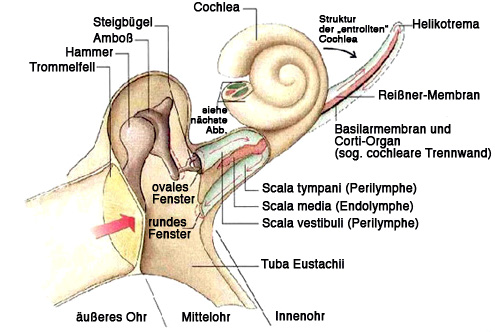
\includegraphics[width = 12cm, height = 8cm]{Ohr_Bild.jpg}
\caption{Schematische Darstellung eines Hörorgans mit abgerollter Kochlea}
\text{\footnotesize{Abruf 25.01.19 \url{http://www.eclim.de/AkuLNew/roomac_1n.html}}}
\label{fig:Ohr_Bild}
\end{figure}


Das menschliche Gehör ist in der Lage Schallereignisse mit Frequenzen von ca. 20Hz bis 16kHz - 20kHz wahrzunehmen. Dabei nimmt die Fähigkeit hohe Frequenzen zu hören um ca. 1kHz pro Lebensdekade durch Abnutzung der Haarzellen mit dem Alter ab \cite[S.41]{Genuit10}.  \\

\begin{figure}[H]
\centering
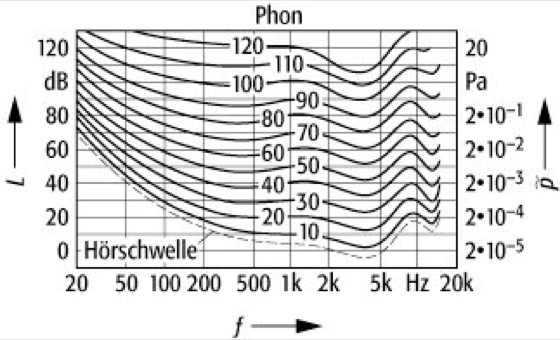
\includegraphics[width = 12cm, height = 8cm]{Kurven_gleicher_Lautheit.jpg}
\caption{Kurven gleicher Lautheit}
Die Hörereignisse einer durchgezogenen Linie werden, trotz unterschiedlichen Schalldruckpegels gleich laut wahrgenommen. Die oberste Linie stellt die Schmerzschwelle und die unterste die Ruhehörschwelle dar.
\text{
\footnotesize{Abruf 25.01.19 \url{https://www.spektrum.de/lexikon/physik/kurven-gleicher-lautstaerke/8648}}}
\label{fig:Kurven_gleicher_Lautheit}
\end{figure}

Der Dynamikbereich des menschlichen Gehörs wird durch die Ruhehörschwelle und die Schmerzschwelle eingegrenzt und kann hierbei frequenzabhängig zwischen 120 dB und 140 dB umfassen. Die Kurven gleicher Lautheit, siehe Abbildung \ref{fig:Kurven_gleicher_Lautheit}, zeigen, dass Schallereignisse je nach Frequenz unterschiedlich laut wahrgenommen werden. Diese Frequenzabhängigkeit der empfundenen Lautheit basiert auf der Anatomie des menschlichen Ohres. Im mittleren Frequenzbereich (1 kHz bis 5 kHz) ist das menschliche Ohr am empfindlichsten. Dies ist deutlich daran zu erkennen, dass für die gleiche empfundene Lautheit bei tiefer- bzw. höherfrequenten Schallereignissen ein deutliche höherer Schalldruckpegel erreicht werden muss. Außerdem ist in diesem Bereich die Dynamik zwischen Hörschwelle (0 Phon) und Schmerzgrenze (120 Phon) am höchsten. Dies ist evolutionsbiologisch darauf zurückzuführen, dass sowohl viele Umgebungsgeräusche als auch für das Sprachverständnis wichtige Konsonanten in diesem Frequenzbereich liegen \cite[S.47]{HdA08}. 

\subsection{Verarbeitung akustischer Signale vom zentralen Nervensystem}

Die im zentralen Nervensystem eintreffenden Signale bilden, nach der Ortstheorie des Hörens, nur ein bestimmtes Frequenzband ab. Die elektrischen Signale lassen sich daher als durch Bandpassfilter verschiedener Bandbreite und Güte,  gefilterte Signale betrachten, wobei das menschliche Gehör in der Lage ist die Parameter an die zu analysierende Szene adaptiv anzupassen \cite[S.59]{Genuit10}. \\

Die Verarbeitung im zentralen Nervensystem erfolgt nach dem Prinzip der Mustererkennung. Die Signale werden spektral analysiert, um Merkmale zu extrahieren, anschließend bestimmte Muster zu identifizieren und wiederzuerkennen \cite[S.51]{HdA08}. Die Betrachtung der neuronalen Prozesse zur Mustererkennung soll im Rahmen dieser Arbeit nicht weiter erläutert werden. Wichtig zu sagen ist jedoch, dass  zur Analyse von Schallereignissen frühere Wahrnehmungen, Erfahrungen, sowie andere Sinnesreize herangezogen werden. Jeder Mensch greift somit auf unterschiedliche Erfahrungswerte zurück, weshalb der Aspekt der individuellen Wahrnehmung bei der Erstellung multimedialer Inhalte stets berücksichtigt werden muss. 

\section{Räumliche Wahrnehmung}
Zur Lokalisation von Hörereignissen und deren Ausdehnung werden Schallsignale nach bestimmten Merkmalen ausgewertet. Die am Trommelfell eintreffenden Schallsignale können hierbei in monoaurale und interaurale Ohrsignale kategorisiert werden. Zum Empfang monoauraler Ohrsignale ist ein Ohr ausreichend, während für den Empfang interarualer Ohrsignale beide Ohren benötigt werden. Die räumliche Wahrnehmung erfolgt sowohl durch die Analyse monoauraler als auch interauraler Ohrsignale, wobei das interaurale Hören hauptsächlich für die horizontale und das monoaurale Hören für die vertikale Wahrnehmung verantwortlich ist \cite[S.88]{HdA08}.\\

\subsection{Kopfbezogene Übertragungsfunktionen}

Das menschliche Gehör kann im technischen Sinne als Antenne betrachtet werden, dessen Richtcharakteristik eine Richtungs- , Entfernungs-  und Frequenzabhängigkeit aufweist \cite[S.89]{HdA08}. Je nach Ort der Schallquelle ändert sich damit Phasengang, Gruppenlaufzeit und Frequenzgang des Schalls, der letztlich am Trommelfell ankommt. Die Veränderung des Schalls von der Quelle des Schallereignisses bis hin zur Senke, also dem Trommelfell, kann mittels sogenannter kopfbezogener Übertragungsfunktionen oder Head-Related Transfer Functions (HRTF's) beschrieben werden. Eine HRTF ist abhängig vom Ort der Quelle, dem Ort der Senke und dem Frequenzspektrum des Schallereignisses. Die Parameter einer HRTF $H(f,r,\phi,\delta))$ sind somit die Frequenz $f$, der Abstand zwischen Trommelfell und Schallereignis $r$ und die kopfbezogenen Richtungswinkel Azimut $\phi$ und Elevation $\delta$. Alle Parameter variieren zwischen dem linken und dem rechten Ohr, so dass immer ein binaurales Paar von HRTF's bzw. eine sogenannte interaurale Außenohr-Übertragungsfunktion $H_i$ betrachten werden muss. Diese setzt sich aus dem Verhältnis der linken HRTF $H_l$ zu der rechten HRTF $H_r$ zusammen \cite[S.91]{HdA08}:

\begin{align}
H_i(f,r,\phi,\delta) = \frac{H_r(f,r,\phi,\delta))}{H_l(f,r,\phi,\delta)}
\end{align}

 Die kopfbezogenen Übertragungsfunktionen sind auf Grund der unterschiedlichen Formen von Kopf, Schultern und Außenohren des Menschen sehr individuell. In Abbildung \ref{fig:HRTF} ist dies besonders im Frequenzbereich über 7kHz zu erkennen, da die Schalldruckpegel hier sehr stark zwischen den bei Probanden gemessenen HRTF's variieren. 

\begin{figure}[H]
\centering
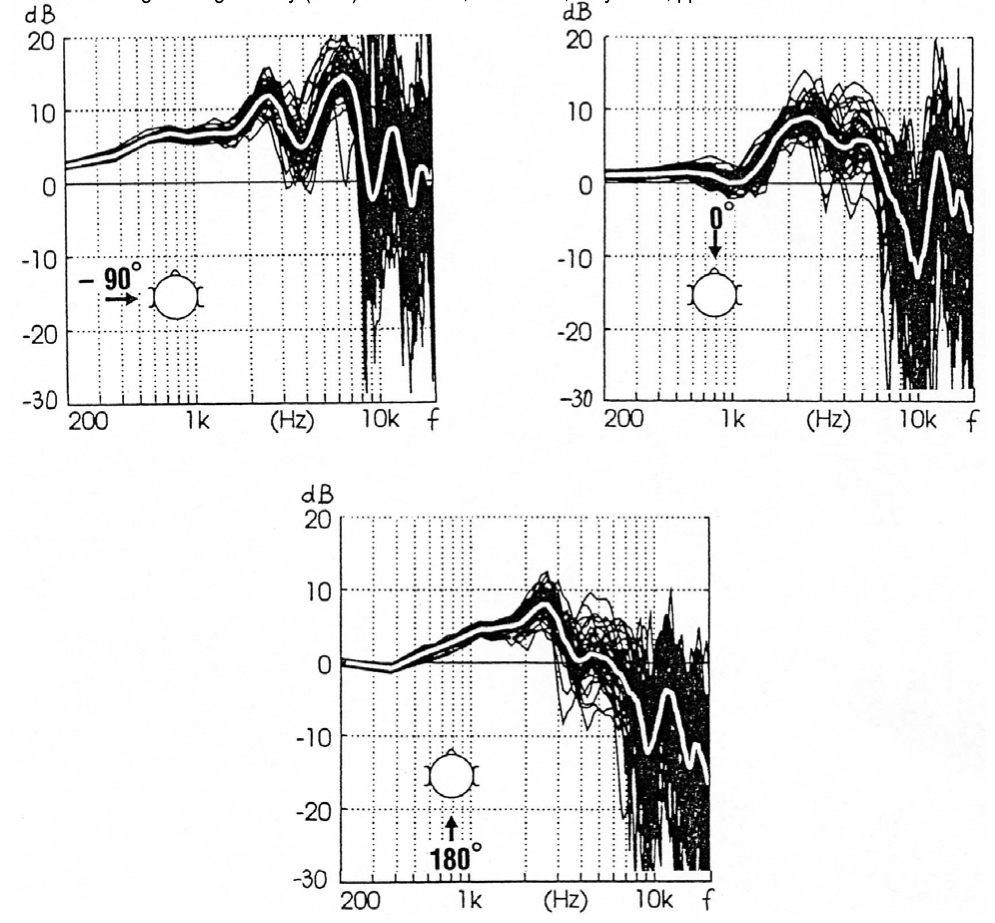
\includegraphics[width = 9cm, height = 9cm]{HRTF.jpg}
\caption{Kopfbezogene Übertragungsfunktionen eines linken Ohres}
Es wurden HRTF's mehrerer Personen für unterschiedlicher Richtungen aufgenommen. Die weißen Kurven entsprechen dem bewerteten Mittelwert. Auffälig ist besonders die Varianz im Frequenzbereich über 7 kHz.
\text{ \footnotesize{Abruf 25.01.19 \url{http://www.sengpielaudio.com/KopfbezogeneUebertragungsfunktionHRTF.pdf}}}

\label{fig:HRTF}
\end{figure}

\subsection{Größen des binauralen Hörens}
Wichtige Merkmale, die zur Lokalisation eines Schallereignisses analysiert werden, lassen sich aus der interauralen Außenohr-Übertragungsfunktion bestimmen. Nach Brauert und Braasch werden diese Größen des binauralen Hörens wie folgt berechnet \cite[S.91]{HdA08}:

\subsubsection{Interaurale Laufzeitdifferenzen}
Die interaurale Phasenlaufzeit oder auch interaurale Laufzeitdifferenz $\tau_{ph}$ berechnet sich aus dem Verhältnis der interauralen Phasendifferenz $\Delta L_i$, also der Differenz der Phase von linker zu rechter HRTF, zur Frequenz $f$ des Schallereignisses: 

\begin{align}
\tau_{ph}(f,r,\phi,\delta) = \frac{\Delta\delta_i(f,r,\phi,\delta))}{f}
\end{align}

Anhand der interauralen Laufzeitdifferenz lässt sich bestimmen an welchem Ohr der Schall bestimmter Frequenzen zuerst ankommt. Dies ist ein, für den Menschen, wichtiges Merkmal für die Lokalisierung des Schallereignisses, da beispielsweise von links kommender Schall auch zu erst beim linken Ohr auftritt.

\subsubsection{Interaurale Gruppenlaufzeit}
Für die interaurale Gruppenlaufzeit wird das Verhältnis der Ableitung der interauralen Phasendifferenz zur Frequenz $f$ des Schallereignisses berechnet: 
\begin{align}
\tau_{gr}(f,r,\phi,\delta) = \frac{d\Delta\delta_i(f,r,\phi,\delta))}{f}
\end{align}

Die interaurale Gruppenlaufzeit gibt im Gegensatz zur interauralen Laufzeitdifferenz an, bei welchem Ohr die Einhüllende des Schallereignisses zu erst ankommt und wie stark verzögert sie das zweite Ohr erreicht. 


\subsubsection{Interaurale Pegeldifferenzen}

Die interaurale Pegeldifferenz $\Delta L_i$ wird als logarithmisches Maß zur Beschreibung der Intensitätsunterschiede des Schalls verwendet, der an beiden Ohren ankommt: 

\begin{align}
\Delta L_i = 20* \lg(H_i(f,r,\phi,\delta)) 
\end{align}


\subsection{Schallquellenlokalisation}

Das Außenohr, der Kopf und die Schultern wirken alle als richtungs-, entfernungs- und , frequenzabhängige Filter für den am Trommelfell eintreffenden Schall. Ist dem Hörenden ein Schallereignis bekannt, so ist er in der Lage die Filterung zu analysieren und anhand der Akustik des Schalls Rückschlüsse auf die Position des Schallereignisses zu ziehen.

\begin{figure}[H]
\centering
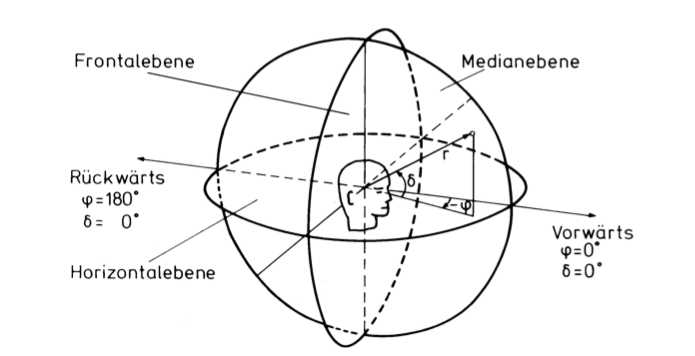
\includegraphics[width = 12cm, height = 6cm]{kopfbezogenes_Koordinatensystem.png}
\caption{Kopfbezogenes Koordinatensystem}
\text{Nach Blauert und Braasch \cite[S.88]{HdA08}}
\label{fig:Kopfbezogenes_Koordinatensystem}
\end{figure}

\subsubsection{Richtungswahrnehmung}

Schallquellen innerhalb der Frontal- und Horizontalebene können anhand von interauralen Laufzeitdifferenzen, interauralen Pegeldifferenzen sowie interauralen Gruppenlaufzeitunterschieden lokalisiert werden. Der Kopf des Menschen weist eine Filtercharakteristik für hohe Frequenzen auf. Wellenlängen, die kleiner als der Kopf selbst sind, werden durch diesen gedämpft. Die Ortung hoher Frequenzen erfolgt daher weitestgehend durch die Analyse der Gruppenlaufzeit und der Pegeldifferenzen, da die Einhüllende des Schalls durch den Kopf weniger stark beeinflusst wird. Die Lokalisierung niederfrequenten Schalls erfolgt dahingehend durch die Verarbeitung der Laufzeit- und Pegeldifferenzen \cite[S.45]{Genuit10}. \\ 

Die monoauralen Außenohrübertragungsfunktionen weisen aufgrund der Struktur des Außenohres eine signifikante Abhängigkeit zum Einfallswinkel des Schalls auf. Dadurch ist es dem Menschen erlaubt schon geringe Positionsänderungen der Schallquelle zur Medianebene wahrzunehmen \cite[S.46]{Genuit10}. \\ 

Die horizontale Wahrnehmung ist empfindlicher als die vertikale Wahrnehmung. In der Horizontalebene werden Richtungsänderungen ab ca. 4 grad und in der Frontalebene erst ab ca. 10 grad merklich wahrgenommen \cite[S.95]{HdA08}.  \\

Die Lokalisation von Schallquellen in der Medianebene  basiert auf der Verarbeitung monoauraler Merkmale, da durch die Position der Schallquelle der Direktschall für beide Ohren annähernd identisch ist. Auch hier gilt, dass die Filterwirkung von Außenohr und Körper, speziell die Schultern, den Schall so beeinflussen, dass Änderungen des Klangs zur Richtungslokalisation interpretiert werden können \cite[S.46]{Genuit10}. \\

Wellenlängen, die größer als die Ohrmuschel selbst sind, werden durch das Ohr kaum beeinflusst. Daraus resultiert, dass die Filterwirkung des Außenohres sich auf Frequenzen oberhalb von ca. 3,5 kHz begrenzt. Die Richtungslokalisation von Schallquellen in der Horizontal- und Frontalebene erfolgt daher besonders gut bei höherfrequenten Schallereignissen \cite[S.47]{Genuit10}.

Ein wichtiger Aspekt der Richtungslokalisation ist die Fähigkeit des Menschen seinen Kopf zu bewegen. Die dadurch entstehenden Änderungen der interauralen Laufzeit- und Intensitätsdifferenzen lassen sich zeitlich analysieren, so dass die Richtung des Schalls leichter erkannt werden kann \cite[S.88]{HdA08}.

\subsubsection{Entfernungswahrnehmung}

Wie bei der Richtungslokalisation gelingt auch das Entfernungshören aufgrund der Verarbeitung von mono- sowie interauralen Merkmalen.

Ist die Schallquelle dem Hörenden sehr nahe (weniger als 25cm entfernt) so bewirkt die Abschirmung durch den Kopf, dass der Schall bei einem Ohr stark gedämpft ankommt. Die interaurale Pegeldifferenz ist daher für die Entfernungseinschätzung naher Schallquellen von herausragender Bedeutung \cite[S.98]{HdA08}.\\

Des Weiteren wird auch der allgemeine Signalpegel zur Entfernungseinschätzung genutzt. Ist ein Signal leiser so ist davon auszugehen, dass die Quelle weiter entfernt ist \cite[S.98]{HdA08}.\\

Ist die Schallquelle zwischen 25cm und 15m vom Hörer entfernt, spricht man vom mittleren Entfernungsbereich. Bei Kugelstrahlern 0. Ordnung, im freien Schallfeld, erzielt eine Abstandsverdopplung der Quelle zum Hörer, in diesem Bereich, eine Steigerung des Signalpegels um 6dB \cite[S.98]{HdA08}. In einem Raum gilt, dass die Menge an Direktschall, der am Trommelfell ankommt mit der Entfernung abnimmt. Aus diesem Grund ist das Verhältnis von Direktschall zu diffusem Schall ein weiteres informatives Merkmal zur Einschätzung von Entfernungen \cite[S.57]{Heidermanns1979}.
\\

Die Entfernung zu Hörereignissen, die weiter als 15m entfernt sind, kann ohne Hintergrundwissen, wie z.B visuelle Eindrücke, nicht geschätzt werden. Da Schall über weite Entfernung jedoch frequenzabhängig gedämpft wird, lässt sich anhand des dumpfen Klangs beurteilen, ob die Schallquelle weit entfernt sein muss \cite[S.99]{HdA08}. 

\subsection{Im-Kopf-Lokalisation}
Sind die Schallquellen sehr nah, wie z.B bei Kopfhörern, kann es zur sogenannten Im-Kopf-Lokalisation kommen. Das Schallereignis wird hierbei im Kopf statt vor den Ohren lokalisiert. \\ 

Die Filterwirkung des Außenohrs und die Beschallung der Schädelknochen, die ebenfalls vom Gehör analysiert werden kann, fallen bei der zu nahen Beschallung weg. Da dies natürlicherweise nicht vorkommt ist das Gehör nicht daran gewöhnt Schall zu analysieren der nicht durch das Außenohr entzerrt worden ist. Der Im-Kopf-Lokalisation kann daher durch eine vorherige Entzerrung der Ohrsignale entgegengewirkt werden, so dass auch über Kopfhörer der Schall entfernter Schallquellen simuliert werden kann \cite[S.47]{Blauert80}.

\subsection{Schallquellenortung bei mehreren Schallquellen}

Bei der Hörereignisbildung mit mehreren Schallquellen treten verschiedenste Effekte auf. Die wichtigsten Effekte sollen im Sinne dieser Arbeit kurz erläutert werden, um ihren Einfluss beim Hörversuch einschätzen zu können. 

\subsubsection{Summenlokalisation - Phantomschallquellen}

Bei zwei Schallquellen, die das selbe Signal wiedergeben und gleich weit vom Hörenden entfernt sind, siehe Abbildung \ref{fig:Stereoaufstellung_Phantomschallquelle}, wird das Hörereignis zentral zwischen den beiden Schallquellen gebildet. Diese Summenlokalisation der Ohrsignale führt zur Bildung einer imaginären Schallquelle, welche zentral zwischen den realen Schallquellen lokalisiert wird. Diese imaginären Schallquellen werden als Phantomschallquellen bezeichnet  \cite[S.101]{HdA08}. \\

Die Richtungslokalisation ist jedoch bei Phantomschallquellen in der Regel fehleranfälliger als bei realen Schallquellen. Dies gilt besonders bei der seitlichen Bildung von Phantomschallquellen mit Surround-Sound  \cite[S.103]{HdA08}. 

\begin{figure}[H]
\centering
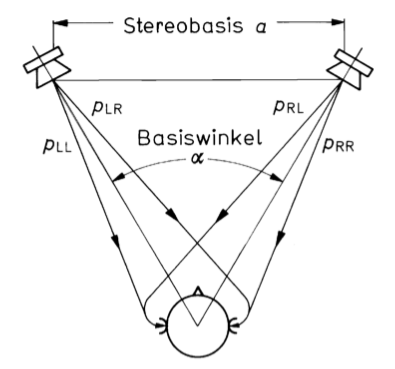
\includegraphics[width = 8cm, height = 6cm]{Stereoaufstellung_Phantomschallquelle.png}
\caption{Stereolautsprecher-Anordnung} 
Sind zwei Schallquellen gleich weit vom Hörenden entfernt und spielen gleichzeitig das gleiche Signal ab, dann bildet sich das Hörereignis zentral zwischen den Schallquellen.
\text{\cite[S.101]{HdA08}}
\label{fig:Stereoaufstellung_Phantomschallquelle}
\end{figure}

Bei der Summenlokalisation werden Laufzeit- und Pegeldifferenzen zwischen den beiden Lautsprechersignalen analysiert, um die Phantomschallquelle zu lokalisieren. Ist ein Signal stärker als das andere  wird die Phantomschallquelle eher in Richtung der lauteren, realen Quelle lokalisiert. Gleichzeitig wird die Phantomschallquelle eher in Richtung der realen Schallquelle lokalisiert, dessen Schall früher beim Hörenden ankommt. Bei größeren Verzögerungen kommt es zum sogenannten Präzedenzeffekt. Dieser wird im Folgenden noch erläutert. \\ 

Anhand der Abbildung \ref{fig:Summenlokalisationskurven} lässt sich erkennen, dass die Richtungszuordnung in keinem linearen Zusammenhang zu wahrgenommenen Laufzeit- und Pegeldifferenzen steht. Des Weiteren ist zu erwähnen, dass sich die Auswirkung der Laufzeit- und Pegeldifferenzen gegenseitig beeinflussen und aufheben können \cite[S.103]{HdA08}. 
 
\begin{figure}[H]
\centering
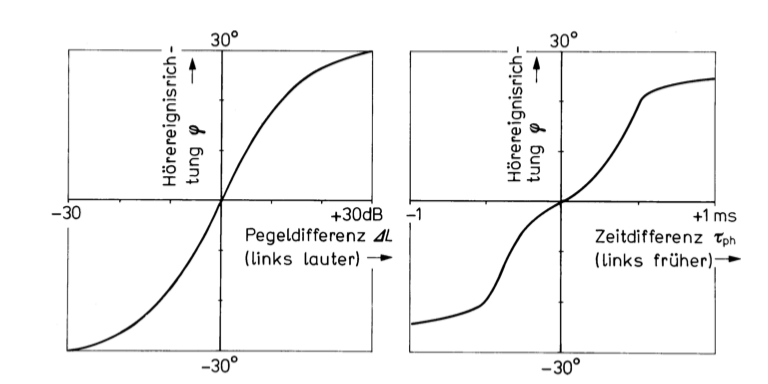
\includegraphics[width = 14cm, height = 8cm]{Summenlokalisationskurven.png}
\caption{Summenlokalisationskurven für Pegel- und Laufzeitdifferenzen der beiden Lautsprechersignale} 
Die Richtungslokalisation wird von Laufzeit- und Pegeldifferenzen nicht-linear beeinflusst. Beide Größen können sich hierbei gegenseitig aufheben. 
\text{\cite[S.101]{HdA08}}
\label{fig:Summenlokalisationskurven}
\end{figure}

\subsubsection{Präzedenzeffekt}

Bei der Wiedergabe eines Signals über mehrere Lautsprecher wird, nach dem Gesetz der ersten Wellenfront, die Hörereignisausrichtung fast ausschließlich anhand des ersten eintreffenden Schalls vorgenommen. Die Signale, die mit mehr als einer Millisekunde Verzögerung eintreffen werden dann als indirekter Schall gewertet, so dass dieser nur zur Lautheitswahrnehmung beiträgt und nicht zur Richtungslokalisation. Dies ermöglicht es auch in geschlossen Räumen ein Hörereignis trotz mehrfach reflektierten Schalls zu lokalisieren \cite[S.103]{HdA08}. \\

Treffen Signale mit einer Verzögerung von mehr als 50 ms auf, wird der Schall nicht als indirekter Schall sondern als Echo erkannt. Dies bewirkt, dass der Schall nicht in die Summenlokalisation für die Position der ersten Quelle  mit einbezogen wird, sondern stattdessen als einzelnes Hörereignis mit eigener Quelle erkannt wird. Besitzt ein Signal einen deutlichen höheren Pegel als die vorherigen Signale kann es auch bei einer geringeren Verzögerung als 50ms zur Echobildung kommen \cite[S.49]{Genuit10}. 
 

\subsubsection{Binaurale Störgeräuschunterdrückung - Cocktailparty-Effekt}

Der Mensch ist in der Lage den Schall in seiner Umgebung zwischen Nutzschall und Störgeräuschen zu unterscheiden. Durch die Lokalisation der Nutzschallquelle, z.B. einer sprechenden Person, kann bewusst die Wahrnehmung anderer Störschallquellen unterdrückt werden (Cocktailparty-Effekt). Die Analyse interauraler Laufzeit- und Pegeldifferenzen ermöglicht eine Dämpfung des Störschalls zwischen 9 und 15 dB. Die Effektivität der Störschallunterdrückung ist abhängig von der Richtung des einfallenden Schalls \cite[S.48]{Genuit10}. 

\section{Zusammenspiel mehrerer Sinnesreize }
Für die Deutung der akustischen Signale vom zentralen Nervensystem werden, neben den akustischen, weitere Sinnesreize herangezogen. Im Rahmen des Hörversuches dieser Arbeit werden Probanden sowohl optischen als auch akustischen Sinnesreizen unterzogen. Wie sich die Wahrnehmungen dieser Reize gegenseitig beeinflussen und welche Effekte hierbei auftreten können, soll im Folgenden erläutert werden.

\subsection{Einfluss des Visuellen auf die auditive Wahrnehmung}
Die Einordnung des Schallereignisses mittels einer Mustererkennung im Gehirn des Menschen basiert darauf, dass Merkmale aus den aktuell eintreffenden Reizen gebildet werden. Solch ein Merkmal könnte beispielsweise eine bestimmte spektrale Zusammensetzung sein. Die Menge aller Merkmale wird daraufhin mit Merkmalen vergangener Ereignisse verglichen. Korreliert hierbei eine Merkmalsmenge mit der eines vergangen Ereignisses, so kann das Zentrale Nervensystem das Schallereignis kategorisieren und einordnen \cite[S.51]{HdA08}. \\ 

Neben akustischen Merkmalen werden auch aus visuellen Reizen Merkmale gebildet \cite[S.88]{HdA08}. Die Wahrnehmungsfähigkeit des Menschen steigert sich durch den Einsatz mehrerer Sinnesreize enorm, da es dem zentralen Nervensystem so ermöglicht eine größere Menge an Merkmalen zu bilden, irrelevante Merkmale leichter auszusortieren und auf einen größeren Erfahrungsschatz zurückzugreifen. \\ 

\subsection{Hörausrichtung an Blickrichtung}

Neben diesem psychologischen Aspekt, muss der physiologische Aspekt der Anpassung der Richtcharakteristik des Gehörs an die Blickrichtung mit herangezogen werden. Der Mensch ist nachweislich in der Lage sowohl die Ausrichtung des Trommelfells als auch die Stellung der Haarzellen in der Kochlea an die  Blickrichtung anzupassen, um Hörereignisse, auf die er sich fokussiert, besser hören zu können. Dabei geschieht die Ausrichtung der Gehörkomponenten sogar vor dem Wechsel des Blickpunkts\cite{Strick17}. Eine Visualisierung der akustischen Szene kann also dafür sorgen, dass gezielt bestimmte Inhalte besser gehört werden können, in dem diese visuell Aufmerksamkeit auf sich ziehen.  

\subsection{Bauchredner-Effekt}

Treffen akustischer und optischer Reiz synchron, also mit einer Verzögerung von maximal ca. 50- 100ms,  auf können sich die individuellen Wahrnehmungen gegenseitig beeinflussen. Für die Deutung der auditiven Merkmale ist der optische Reiz hierbei von größerer Bedeutung als es umgekehrt der Fall ist. Bauchredner versuchen auf diese Weise dem Publikum die Lokalisation der wahren Schallquelle zu erschweren. Der sich bewegende Mund der Puppe stellt einen visuellen Reiz dar, der mit dem Hörereignis des sprechenden Redners übereinstimmt. In Folge dessen wird die wahrgenommene Schallquelle auf den Mund der Puppe projiziert \cite[S.163]{Genuit10}.

Obwohl visueller und auditiver Reiz nicht zusammen passen wird die Gesamtsituation vom Konsumenten als plausibel wahrgenommen. Dies bedeutet, dass ein perfektes Panning der auditiven Signale für eine plausible Wiedergabe nicht immer von Nöten ist. Andererseits ist aber auch zu beachten, welchen visuellen Reizen der Betrachter im Moment der auditiven Wiedergabe untersetzt ist. Schaut der Betrachter im Moment der auditiven Wiedergabe auf eine potentielle, alternative Schallquelle  kann eine ungewollter Fehllokalisation der Hörereignisse stattfinden kann.


\section{Wohlbefinden bei akustischen Szenen}
Damit virtuell erstellte Medien beim Kunden Anklang finden, müssen diese sich beim Konsum vor allen Dingen wohlfühlen. Gerade im Bereich AR und VR geht es oft darum, dass auditive und visuelle Inhalte so realistisch wie möglich dargestellt werden sollen, dabei ist bereits bewiesen, dass zu realistische, visuelle Szenen eher Unbehagen als Begeisterung beim Betrachter bewirken. Im Rahmen dieser Arbeit soll dahingehend auch geprüft werden inwiefern bei auditiven Szenen solch ein Unbehagen ausgelöst werden kann, in dem überprüft wird wie sich die Versuchsprobanden bei der Darbietung der audiovisuellen Szenen fühlen. 

 \subsection{Immersion}
 Virtual Reality wird häufig mit dem Wort Immersion in Verbindung gebracht. Als Immersion bezeichnet man die Einhüllung in Medien. Im Folgenden soll kurz der Zustand der Immersion erläutert und im Anschluss der Zusammenhang zu den Themen dieser Bachelorarbeit geschlossen werden. \\
Nach Grau äußere sich die Immersion in dem Moment in dem der Betrachter die kritische Distanz zum Medium verliere und die emotionale Involvierung ansteige \cite[S.13]{Grau03}. Der Konsument wird im Zustand der Immersion also Teil der medialen Szene und ist in der Lage seine reale Umgebung komplett auszublenden. Auch wenn dies schon bei älteren Medien wie Fernsehen oder Theater der Fall gewesen ist, so ist es möglich diesen Zustand bei VR und AR noch intensiver zu verwirklichen.  \\

\begin{figure}[H]
\centering
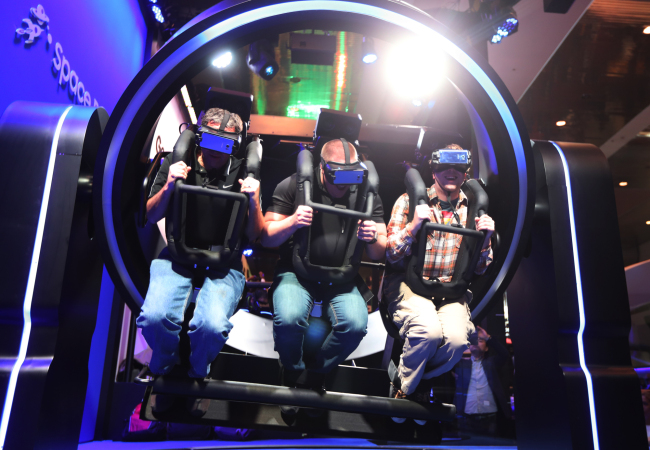
\includegraphics[width = 10cm, height = 6.5cm]{VR_Immersion.jpg}
\caption{Immersives Erlebnis durch Achterbahnsimulation mit der Samsung Gear}
\text{\footnotesize{Abruf 29.01.19: \url{http://forums.cgsociety.org/t/samsung-gear-vr-fully-immersive-4d-experience/1810570}}}
\label{fig:VR_Immersion}
\end{figure}

Virtual Reality biete hierbei Techniken, die traditionelle Medien polysensorisch erlebbar machen würden, behauptet Grau \cite[S.15]{Grau03}.  In diesem Zusammenhang wurde besonders der Aspekt der freien Kopfbewegung genannt, der es ermögliche die Szene aus unendlich vielen Perspektiven zu beobachten. Auch der Einsatz von räumlichem Audio sowie die Interaktion mit der virtuellen Welt erlaube ein noch stärkeres Gefühl der Immersion \cite[S.16]{Grau03}. \\
 
 Damit die synthetisch erschaffene Welt eine Immersion zulasse, müsse diese nicht die Umgebung komplett umfassen, beziehungsweise realistisch sein, sondern stattdessen plausibel\cite[S.17]{Grau03}. Die Stärke der Immersion hänge dabei zum einen von der Glaubwürdigkeit, aber auch von der Genießbarkeit der Illusion ab\cite[S.17]{Grau03}. \\
 
 Die Immersion ist im Zusammenhang mit dem Einsatz von räumlichem Audio ein erstrebenswerter Zustand für den Konsumenten. Dieser soll den Eindruck vermittelt bekommen, dass die ihm dargebotene virtuelle Szene Wirklichkeit sein könnte, so dass dieser die Realität ausblendet.
 
In den Versuchen dieser Arbeit soll eine virtuelle Welt in die reale Welt integriert werden. Hierbei werden visuelle und auditive Inhalte im Raum platziert und über eine Microsoft Mixed-Reality-Brille wiedergegeben. In diesem Zusammenhang würde eine Immersion bedeuten, dass der Betrachter die dargebotenen, virtuellen Inhalte als Teil seiner realen Umgebung wahrnimmt. 
 
 Nicht nachvollziehbare Reize können eine Immersion beim Konsumenten verhindern\cite[S.17]{Grau03}. Im Zusammenhang mit den Versuchen bedeutet dies, dass sowohl auditive und visuelle Inhalte, als auch reale und virtuelle Welt zueinander kompatibel sein müssen und plausible Sinneseindrücke bewirken müssen. 
 
 Um das Immersionsempfinden der Probanden während des Hörversuchs zu überprüfen werden, die Probanden gebeten Fragen zu beantworten die Aufschluss über die Plausibilität, den Realismus der auditiven Inhalte und das Wohlbefinden der Probanden, während der Darbietung, geben sollen. 
 
 \vspace*{20pt}
\subsection{Das Uncanny Valley und der Bezug zur Immersion bei VR und AR}

Das \glqq Uncanny Valley \grqq{} ist ein Begriff der Robotik, der zum ersten mal vom japanischen Robotiker Masahiro Mori 1970 verwendet worden ist. Dieser beschreibe die verminderte Vertrautheit des Menschen gegenüber synthetisch erstellten Figuren, wenn diese eine bestimmte Intensität des Anthropomorphismus (Menschenähnlichkeit) aufweisen \cite{Mori70}.\\


Wie in Abbildung \ref{fig:Mori_Uncynn_Valley_de} zu erkennen ist steigt die Akzeptanz des Betrachters gegenüber der visuellen Erscheinung zunächst mit steigernder Menschenähnlichkeit an, bis sie abrupt, ab einem bestimmten Realitätsgehalt, in eine starke Befremdlichkeit übergeht. Anschließend steigt diese Vertrautheit jedoch wieder mit der Menschenähnlichkeit an. Bei bewegten Figuren ist dieser Effekt noch stärker zu beobachten. Der Bereich des starken Abfalls und Wiederanstiegs der Vertrautheitskurve wird als\glqq Uncanny Valley \grqq{} bezeichnet \cite{Mori70}.\\

\begin{figure}[H]
\centering
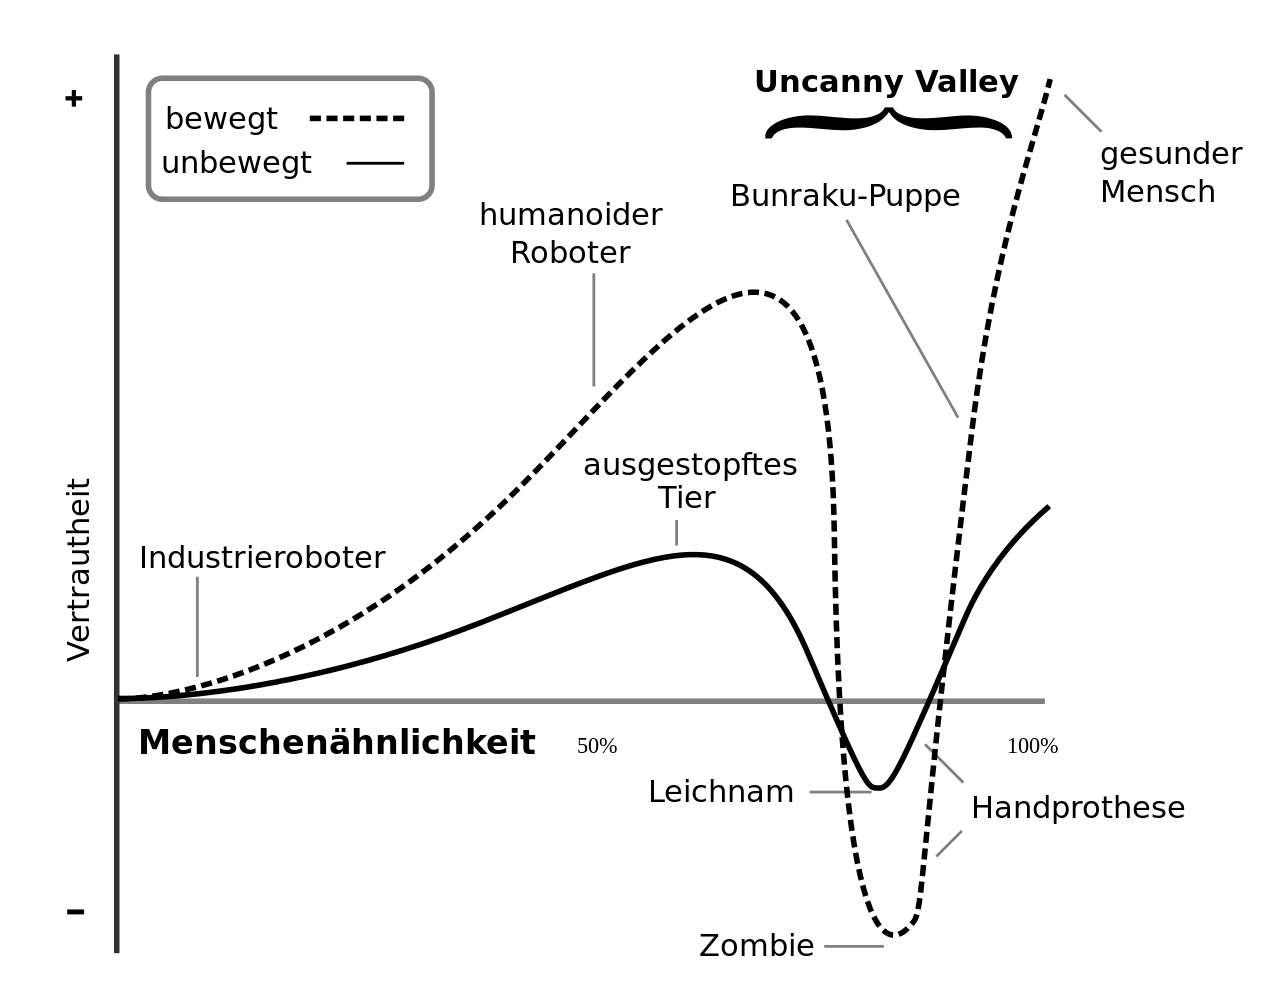
\includegraphics[width = 9.5cm, height = 6.7cm]{Mori_Uncanny_Valley_de.png}
\caption{Darstellung des \glqq Uncanny Valley \grqq{} mit Einordnung verschiedener Figuren} 
Mit steigendem Realismus menschenähnlicher Figuren nimmt die Vertrautheit bis zu einem Minimum ab. Nur wirklich realistische Figuren wirken unbefremdlich. Das Tal der geringen Vertrautheit wird als \glqq Uncanny Valley \grqq{}bezeichnet. 
\text{Abbildung von Mori 1970 $ - $Übersetzung durch Tobias K.}
\text{\footnotesize{Abruf 23.01.19: \url{https://de.wikipedia.org/wiki/Datei:Mori_Uncanny_Valley_de.svg}}}
\label{fig:Mori_Uncynn_Valley_de}
\end{figure}


Die Akzeptanzlücke gegenüber realistischen, synthetisierten, visuellen Reizen, die beim Menschen von Mori beobachtet worden ist, lässt vermuten, dass die Befremdlichkeit gegenüber synthetisierten Szenen, sowohl visuell als auch auditiv, mit dem Realitätsgehalt der Medien zunehmen könnte. \\ 

Große Firmen der Unterhaltungsindustrie wie Sony und Oculus rieten Entwicklern daher schon auf der Game Developers Conference in Köln 2014, dass diese ihre VR-Anwendungen nicht zu realistisch gestalten dürfen, da der Effekt des \glqq Uncanny Valley \grqq{} drohe. Des Weiteren dürfe man die Blickrichtung des Benutzers nicht einschränken und müsse Phobien wie Klaustrophobie oder Höhenangst beachten. VR-Erlebnisse sollen demnach "eher als Analogie zu einem Ritt durch einen Vergnügungspark begriffen werden als zu einem Kinofilm" \cite{Gieselmann}. \\
 
Im Zuge dieser Arbeit werden Audioszenen betrachtet die extremen Realismus implizieren könnten. Es ist nicht auszuschließen, dass auch mit steigendem Realitätsgehalt auditiver Szenen speziell räumlichem Audio eine Art "Uncanny Valley"-Effekt beim Hörenden entsteht. In Anbetracht dessen solltet es umso wichtiger sein, während des Hörversuchs, das Wohlempfinden der Probanden zu beobachten.  Die Erforschung, ob es wirklich ein Art "Uncanny Valley"-Effekt für räumliches Audio gibt, ist ein wichtiges Thema für die Weiterentwicklung von AR und VR und soll Bestandteil dieser Bachelorarbeit werden. 
 
 \chapter{Technische Grundlagen}
Der im Rahmen dieser Arbeit durchzuführende Hörversuch beinhaltet einen typischen Anwendungsfall für eine AR-Anwendung. Eine virtuelle Welt wird mit Hilfe einer Microsoft Mixed Reality Brille auf einen realen Tisch projiziert.  Es folgt die binaurale Wiedergabe von Schallereignissen über virtuelle Punktschallquellen im Raum, die es von den Probanden zu lokalisieren gilt. Ziel hierbei soll sein, die Lokalisationsfähigkeit und das Darbietungsempfinden der Probanden bei räumlichem Audio für einen realistischen Anwendungsfall zu analysieren. Dafür ist eine AR-Applikation entwickelt worden, mit der die Durchführung und Dokumentation des Hörversuchs automatisiert worden ist.

Die zur Erstellung der Applikation notwendigen technischen Grundlagen sowie die verwendete Hard- und Software sollen im Folgenden veranschaulicht werden. 

 \section{Augmented Reality}
Die Erweiterte Realität , engl. Augmented Reality (AR), ist eine Variation der Virtuellen Realität, engl. Virtual Reality (VR). Während bei VR-Anwendungen versucht wird den Benutzer komplett in einer synthetisierten Welt eintauchen zu lassen, geht es bei AR darum die physische Welt des Benutzers virtuell zu ergänzen \cite{Azura97}. \\

\begin{figure}[H]
\centering
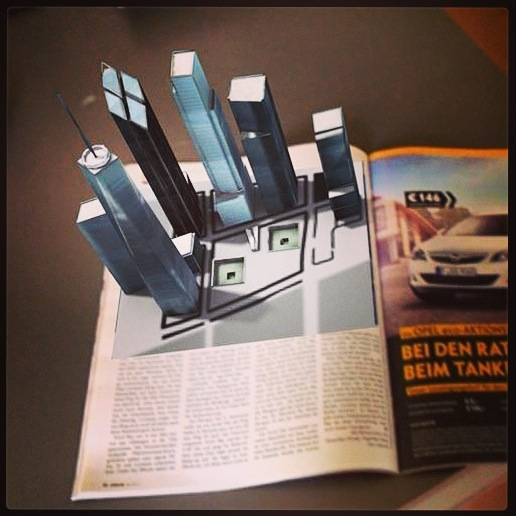
\includegraphics[width = 8cm, height = 6cm]{AR_Beispielbild.jpg}
\caption{Zeitschrift dessen Inhalt durch virtuelle Objekte ergänzt wird}
\text{\footnotesize{Abruf 22.01.19:}}
\text{\footnotesize{\url{https://www.dpc-consulting.org/augmented-reality-aktuelle-beispiele-fur-verlage-und-medienhauser/}}}
\label{fig:AR_Beispielbild}
\end{figure}

Im Hörversuch dieser Bachelorarbeit sollen die Probanen in eine AR-Umgebung eintauchen, bei der der reale Raum mit einer audiovisuellen, virtuellen Welt überlagert wird. 
\newpage

\subsection{Microsoft Mixed Reality}
Microsoft verwendet im Zusammenhang mit AR und VR häufig den Begriff Microsoft Mixed Reality und bezeichnet auch ihre Head-Mounted-Displays als Microsoft Mixed-Reality-Brillen. Nach der Dokumentation von Microsoft  beinhaltet Microsoft Mixed Reality neben der virtuellen Erweiterung der Realität auch die Interaktion zwischen Mensch, Maschine und Umgebung \cite{MicrosoftMR}. 


\begin{figure}[H]
\centering
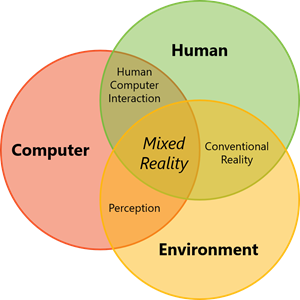
\includegraphics[width = 8cm, height = 8cm]{Mixed_Reality.png}
\caption{Zusammensetzung von Mixed Reality}
Microsoft Mixed Reality ist der Oberbegriff von Microsoft für ihre Augmented und Virtual Reality Hard- und Software. Es zeichnet sich durch das Zusammenspiel von Mensch, Computer und Umgebung aus. 
\text{\footnotesize{Abruf 07.02.19:}}
\text{\footnotesize{\url{https://docs.microsoft.com/en-us/windows/mixed-reality/mixed-reality}}}
\label{fig:Mixed_Reality}
\end{figure}
 
Microsoft bietet mit Microsoft Mixed Reality Gestensteuerung, Spracherkennung, Kopfverfolgung (Head-Tracking), Kopfbezogene Übertragungsfunktionen(HRTF) und weitere Funktionen an. Dabei können sogar auditive und visuelle Inhalte an die physischen Gegebenheiten des Raums angepasst werden. Entwicklern werden diese Funktionen umsonst mit dem MixedRealityToolkit zur Verfügung gestellt, dessen Funktionalitäten wiederum in Unity3D importiert werden können. Auf diese Art und Weise können AR- und VR-Anwendungen erstellt werden, die sowohl räumliches Audio als auch eine an Mixed Reality Brillen angepasste Steuerung ermöglichen. Die wichtigsten verwendeten Funktionen des Toolkits und von Unity3D werden im Verlauf der Arbeit noch individuell betrachtet.

\newpage

\section{Microsoft HoloLens}
Als Wiedergabegerät während des Hörversuchs wird eine Microsoft HoloLens verwendet, siehe Abbildung \ref{fig:microsoft_hololens}. Bei dieser handelt es sich um eine Microsoft Mixed-Reality-Brille, die mit einem Head-Mounted-Display, Kopfhörern, Head-Tracking-Funktion sowie einem Natural-User-Interface ausgestattet ist.

 \begin{figure}[H]
\centering
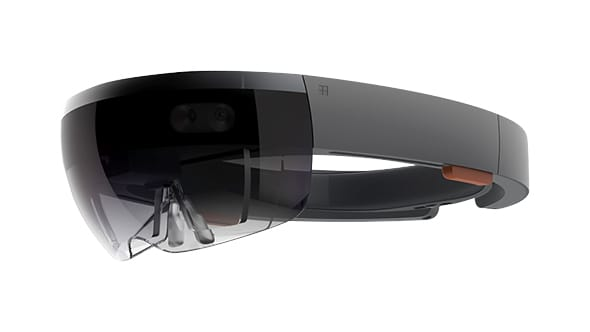
\includegraphics[width = 8cm, height = 6cm]{microsoft_hololens.jpg}
\caption{Mixed-Reality-Brille - Microsoft HoloLens}
\text{\footnotesize{Abruf 23.01.19:}}
\text{\footnotesize{\url{https://www.macerkopf.de/2016/10/12/microsoft-hololens-kommt-im-november-nach-deutschland}}}
\label{fig:microsoft_hololens}
\end{figure}

\subsection{Head-Mounted-Displays}
Für die Umsetzung von AR- und VR-Anwendungen werden sogenannte Head-Mounted-Displays verwendet, welche dem Nutzer ermöglichen sollen möglichst realitätsnah visuelle Reize wahrzunehmen. Die Bildschirme in der Brille projizieren virtuelle Inhalte direkt in das Auge des Benutzers, so dass dieser denken soll Teil der virtuellen Umgebung zu sein. Bei AR-Brillen bzw. der Mixed-Reality-Brille Microsoft HoloLens wird hierbei ein transparenter Bildschirm verwendet, der es ermöglicht neben der virtuellen auch die reale Welt zu sehen.\\


\subsection{Kopfhörer der HoloLens}
Die Kopfhörer befinden sich an der Unterseite des Haltemechanismus der Brille. Sie sind über den Ohren positioniert, bedecken diese aber nicht. Auf diese Weise lassen sie die Umgebungsgeräusche ungedämpft durch. Wie bereits im Unterkapitel "räumliche Wahrnehmung" beschrieben wird, bewirkt die individuelle Außenohrform eine spektrale Verzerrung des Schalls und ist für die spektrale Analyse zur Lokalisation von Hörereignissen von herausragender Bedeutung. Dadurch, dass die Ohren von den Kopfhörern der HoloLens nicht bedeckt werden, ist im Vergleich zu anderen Kopfhörern die frequenzabhängige Filterung der Außenohren gegeben. 

\newpage
\subsection{Head-Tracking-Funktion}
Die HoloLens bietet eine Head-Tracking-Funktion, die es erlaubt die Hörsignale an die Ausrichtung des Kopfes anzupassen. Dies ist wichtig, da die Rotation des Kopfes, neben der offensichtlichen Veränderung des Blickfeldes, auch eine Veränderung des ,an den Ohren ankommenden, Schalls bewirkt. Die Analyse der damit einhergehenden Änderungen der interauralen Laufzeit- und Pegeldifferenzen tragen maßgeblich dazu bei Hörereignisse zu lokalisieren. Die für den Hörversuch entwickelte HoloLens-App erlaubt die freie Bewegung des Probanden im Raum und die freie Bewegung des Kopfes. Auf diese Art und Weise sollte die Lokalisation von virtuellen Schallquellen mit der HoloLens im Vergleich zu statischen Wiedergabesystemen ohne Head-Tracking, stark vereinfacht werden und den Realismus der audiovisuellen Szenen verstärken.  
  
\section{Binaurale Wiedergabe}
 Das Problem der binauralen Wiedergabe räumlicher auditiver Szenen über Kopfhörer ist, dass die Beeinflussung des Schalls durch die Umgebung auf dem Weg zum Trommelfell nicht gegeben ist. Es werden also weder Schallreflexionen, noch die Filterwirkung des Körpers und der Außenohren auf den Schall wahrgenommen. Die Lokalisation von Schallereignissen über Kopfhörer ist dementsprechend nur dann möglich, wenn die binauralen Signale angepasst werden. 
 
 \subsection{Kopfbezogene Übertragungsfunktionen - MS HRTF Spatializer}
 
 Die bereits im Kapitel "Menschliche Wahrnehmung" behandelten kopfbezogenen Übertragungsfunktionen beschreiben das System zwischen der Quelle eines Schallereignissen und der Senke, also dem Trommelfell. Die Faltung des Audio-Signals mit der zugehörigen HRTF verändert den eintreffenden Schall so, als ob er durch den Körper und die Außenohren gefiltert worden wäre. \\
 
Technisch gesehen wird räumliches Audio dadurch realisiert, dass je nach Position der virtuellen Schallquelle zum Kopf ein HRTF-Paar aus einer Datenbank ausgewählt und mit dem wiederzugebenden Audio-Signal digital gefaltet wird. Auf diese Art und Weise werden interaurale Laufzeit- und Pegeldifferenzen dem trockenen Signal hinzugerechnet, so dass auch über  binaurale Wiedergabe eine Schallquellenlokalisation stattfinden kann. Für die Applikation wurde der von Microsoft entwickelte \glqq  MS HRTF Spatializer \grqq{} verwendet, der ebenfalls nach diesem Prinzip arbeitet \cite{MSHRTF}.\\
 
Damit die Lokalisationsfähigkeit bei binauraler Wiedergabe vollständig gegeben ist müsste für jeden Menschen ein individueller Datensatz an HRTF's verwendet werden. Dies spiegelt sich besonders im Bereich der Lokalisation hochfrequenter Schallereignisse wieder, da hier, durch die individuelle Außenohrform, die HRTF's am stärksten variieren. Ein weiterer Ansatz der personalisierten HRTF-Datensätze besteht darin über neuronale Netze und Methoden des Machine Learnings die HRTF-Datensätze automatisch an den Benutzer anzupassen \cite{MSHRTF}.
 
Da die Aufnahme individueller HRTF-Datensätze für jeden Probanden des Hörversuchs den Rahmen dieser Bacherlorarbeit übersteigen würde, wird für die Durchführung ein einzelner HRTF-Datensatz verwendet. Bei der Auswertung der Versuchsergebnisse muss daher berücksichtigt werden, dass der genutzte HRTF-Datensatz unterschiedlich stark mit den wirklichen HRTF-Datensätzen der Probanden korreliert. Dies gilt besonders bei der Betrachtung hochfrequenter Schallereignisse über 7kHz. 
 
 \subsection{Auralisation} 

Auralisation beschreibt Verfahren die es ermöglichen Schallsignale so zu verändern, dass es so klingt als wären diese in einem bestimmten Raum aufgenommen worden. Die Faltung eines Audio-Signals mit der monoaural-aufgenommenen Raumimpulsantwort ermöglicht es den individuellen Klang des gewünschten Raumes  in das Schallsignal zu übertragen und so ein plausible Schallereignisse zu erzeugen  \cite[S.521]{HdA08}.\\

Für AR-Anwendungen in Echtzeit ist dieser Ansatz jedoch eher bedingt geeignet, da sich die Position des Betrachters während der Wiedergabe verändern kann und damit auch eine Anpassung der Raumimpulsantwort in Echtzeit notwendig wäre. \\


\subsubsection{Microsoft - Spatial Audio}
Microsoft bietet mit \glqq  Spatial Audio \grqq{} aus dem MixedRealityToolkit eine alternative Möglichkeit für die Entwicklung von AR-Anwendungen an, die Audio-Signale  an die Umgebung anzupassen. Diese arbeitet mit drei Instanzen, den sogenannten \glqq  Audio Emittern \grqq{} , den  \glqq Audio  Occludern \grqq und einem \glqq Audio Listener \grqq. \\

Spatial Audio nutzt den Effekt, dass hohe Frequenzen des Schalls von Objekten stärker absorbiert werden als niedrige Frequenzen. Aus diesem Grund werden Wände und andere Objekte, die Einfluss auf die Schallausbreitung haben mit Audio Occludern versehen. Diese Skripte steuern Tiefpassfilter mit einer bestimmten Grenzfrequenz und Lautstärkeanpassung. \\

Die Audio Occluder arbeiten Hand in Hand mit den Audio Emittern und dem Audio Listener. In Unity wird jeder Schallquelle ein Audio Emitter zugewiesen, während der Audio Listener nur dem Kamera-Objekt, also dem Nutzer des Head-Up-Displays, übergeben wird. Bei Wiedergabe eines Audio-Signals werden von den Audio Emittern strahlen an die Umgebung abgegeben. Trifft ein Strahl einen Audio Occluder, dann werden von diesem aus ebenfalls Strahlen ausgesendet, die Informationen über die Tiefpasscharakteristik des Objekts enthalten. Beim Audio Listener werden die ankommenden Strahlen ausgewertet. Treffen Strahlen direkt vom Audio Emitter aus den Audio Listener, dann wird dieser als Direktschall gewertet und das Audio-Signal unverändert beim Betrachter wiedergegeben. Bei Strahlen, die von einem Audio Occluder aus gesendet worden sind, wird das Audio-Signal tiefpassgefiltert und lautstärkeangepasst wiedergegeben. Auf diese Weise kann diffuser Nachhall imitiert werden \cite{MSSpatialAudio}.\\

Neben den offensichtlich in der Unity-Szene enthaltenden Objekten, die den Schall mittels Audio Occluder beeinflussen können, müssen bei AR-Anwendung für eine plausibles Hörergebnis die im Raum enthaltenden Objekte, wie Boden, Wände, Tische und Schränke ebenfalls mit Audio Occludern versehen werden. Hierbei gibt es zum einen die Möglichkeit mit \glqq Spatial Mapping\grqq, eine Funktion aus dem MixedRealityToolkit die unmittelbare Umgebung direkt von der HoloLens scannen zu lassen und sich als 3D-Modell ausgeben zu lassen.  Die andere Möglichkeit besteht darin ein eigenes Raummodell mittels 3D-Software zu entwerfen. In beiden Fällen entsteht ein 3D-Modell, welches sich in die Unity-Szene integrieren und durch einen Audio Occluder ergänzen lässt. \\
 
 Für die Applikation des Hörversuchs wurde der zweite Ansatz gewählt, da der Raum zu viele kleine Objekte enthält, bei denen der Scanner der HoloLens Probleme bei der Erstellung eines realitätsnahen Raummodells bekäme.  
 
 \section{Software}
Für die Umsetzung des Hörversuchs der Bacherlorarbeit wurde eine Applikation für die Microsoft HoloLens entwickelt.  Im Folgenden werden  die dafür verwendeten Programme kurz vorgestellt, sowie erklärt welche Funktion diese bei der Erstellung der App gespielt haben. 
 
 \subsection{Blender}
 Blender ist eine freie, Open-Source 3D-Grafiksuite der Blender Foundation zur Erstellung von visuellen Inhalten mittels Animations-, Texturierungs- und Modellierungstools. In den Versuchen dieser Arbeit sollen auditive Szenen visuell unterstützt werden. Die dafür erstellten 3D-Modell wurden alle mit Blender in der Version 2.79b erstellt. 
 
 \begin{figure}[H]
\centering
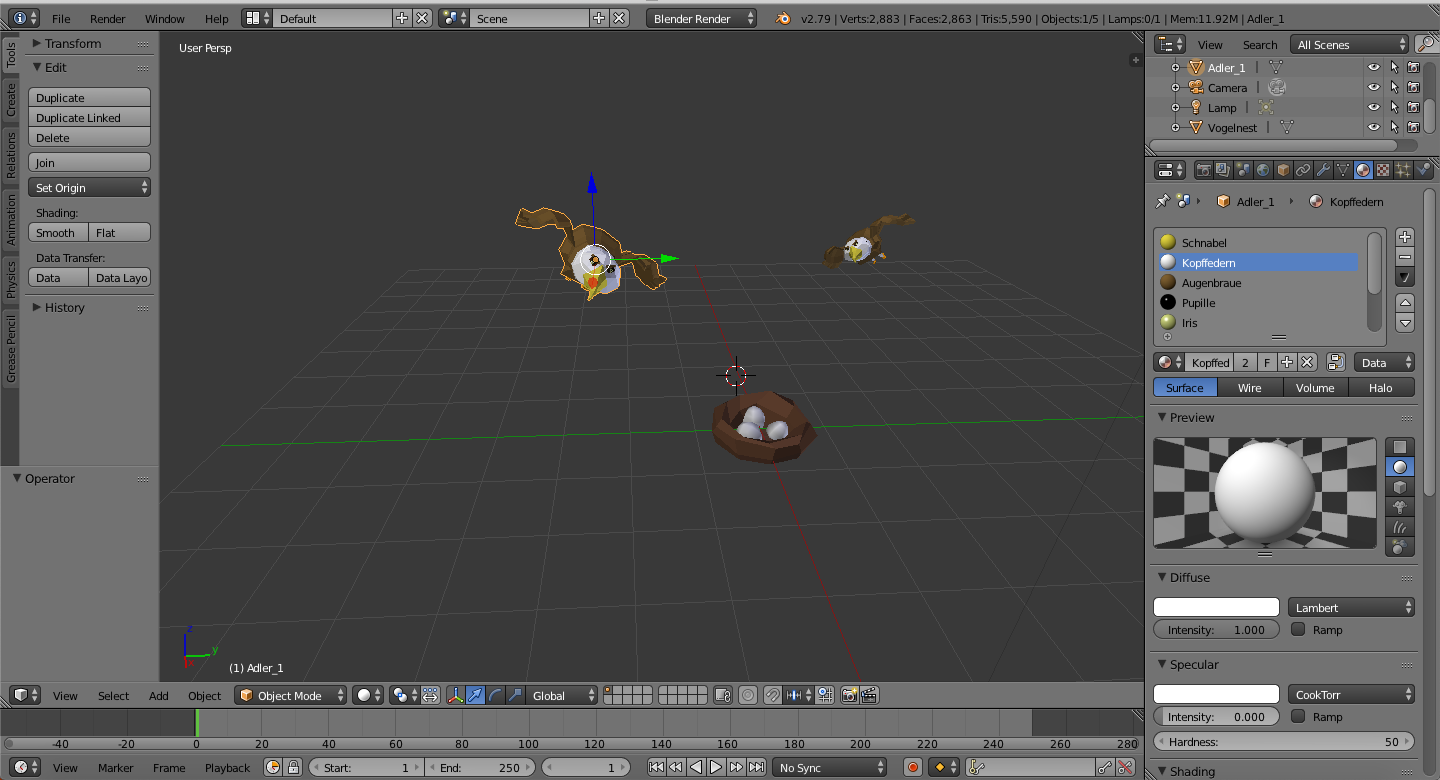
\includegraphics[width = 16cm, height = 9cm]{Blender_Foto.png}
\caption{Benutzeroberfläche von Blender in der Version 2.79}
\label{fig:Blender}
\end{figure} 

\newpage
 \subsection{Unity}
Unity ist eine  Laufzeit- und Entwicklungsumgebung für Spiele, die vom Unternehmen Unity Technologies entwickelt worden ist. Unity bietet Funktionen, die schon seit langem von Unternehmen für professionelle Visualisierungen genutzt werden. Im Rahmen dieser Arbeit bietet Unity die Schnittstelle für die Nutzung der Microsoft HoloLens und den erstellten Animationen . Des Weiteren wird über Unity ein Userinterface für die Durchführung der Versuche entwickelt, welches die Effektivität bei der Durchführung der Versuche steigern soll. Für die Entwicklung der App wurde die Version Unity 2018.3.0f2 verwendet. 

  \begin{figure}[H]
\centering
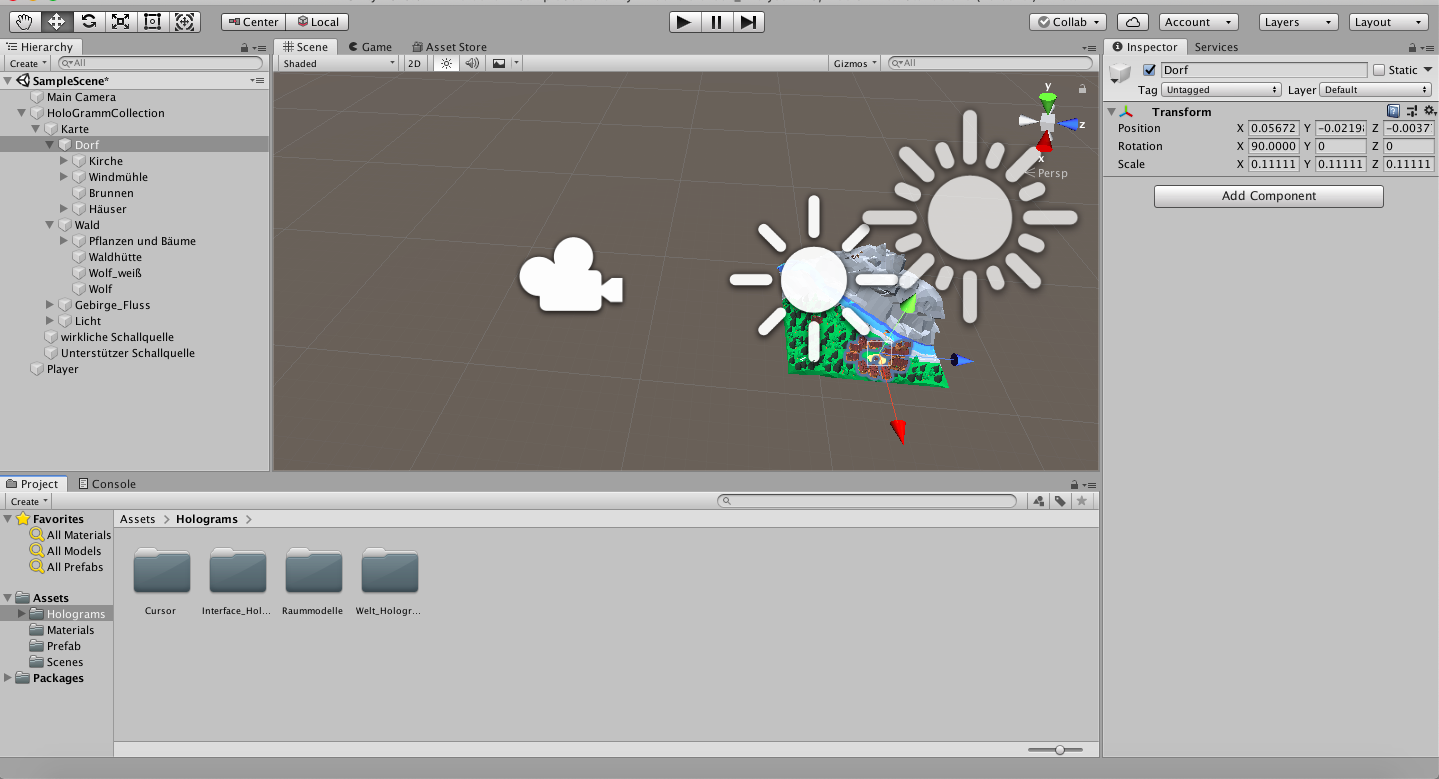
\includegraphics[width = 16cm, height = 9cm]{Unity_Foto.png}
\caption{Benutzeroberfläche von Unity in der Version 2018.3.0f2}
\label{fig:Unity}
\end{figure} 


\chapter{Vorstellung der HoloLens-Applikation und des Hörversuches}

Ziel dieser Arbeit ist es zu überprüfen wie gut bei VR- und AR-Anwendung virtuelle Schallquellen mit räumlichem Audio lokalisiert werden können und wie 3D-Audio bei solchen Anwendungen allgemein angenommen wird. Hierfür wurde ein Hörversuch in einer Mixed-Reality-Umgebung durchgeführt. Die dafür verwendete HoloLens-Applikation wurde mit Unity entwickelt. Im folgenden sollen die App und der Versuchsaufbau vorgestellt werden. 


 \section{Versuchsidee}
 
 Bei dem im Hörversuch nachgestellten Szenario handelt es sich um einen Anwendungsfall für Augmented Reality, wie er auch in der Industrie Anwendung findet. Über das Head-Up-Display der HoloLens werden virtuelle Objekte auf einen Tisch vor dem Nutzer projiziert. Auf diese Weise könnten zum Beispiel virtuellen Prototypen von Maschinen oder Möbeln vorgestellt werden. Neben dem Visuellen spielt auch die auditive Komponente eine beachtliche Rolle.\\ 
 
Software, wie z.B Unity, bietet die Möglichkeit virtuelle Schallquellen an bestimmten Positionen im Raum zu platzieren. Diese sollen dann so klingen als wären diese tatsächlich an der angegeben Position im Raum.  Bei der Vorstellung eines Motorprototypen über AR könnte so z.B eine visuelle aber auch akustische Kostprobe gegeben werden. \\
 
 Wie plausibel diese Softwaretools virtuelle Schallquellen in den Raum projizieren und ob die Konsumenten diese Darbietung überhaupt so annehmen wie gewünscht, soll anhand eines Hörversuches ermittelt werden. \\ 

Besonderer Fokus liegt hierbei auf der Lokalisationsfähigkeit solcher virtuellen Schallquellen sowie auf dem Darbietungsempfinden der Probanden. Dabei soll überprüft werden, ob realistische, räumliche Audio-Darbietungen beim Betrachter Unwohlsein auslösen können, wie es auch bei bestimmten visuelle Reize beim \glqq  Uncanny Valley\grqq{} der Fall ist. 
 
 \newpage
 
 \section{Die virtuelle Welt}
 
Für den Hörversuch wurde eine virtuelle Welt im lowpoly-Grafikstil erstellt. Es handelt sich hierbei um eine  Landschaft mit einem Gebirge, einem Fluss, einem Dorf und einem Waldgebiet. Die Welt ist ca. 1m breit, sowie tief und bis zu 70cm hoch. Im Folgenden werden die einzelnen Gebiete genauer beschrieben. Die dort platzierten Hörereignisse werden jeweils in einzelnen Kapitel vorgestellt. 
\vspace*{30pt}
 
 \begin{figure}[H]
\centering
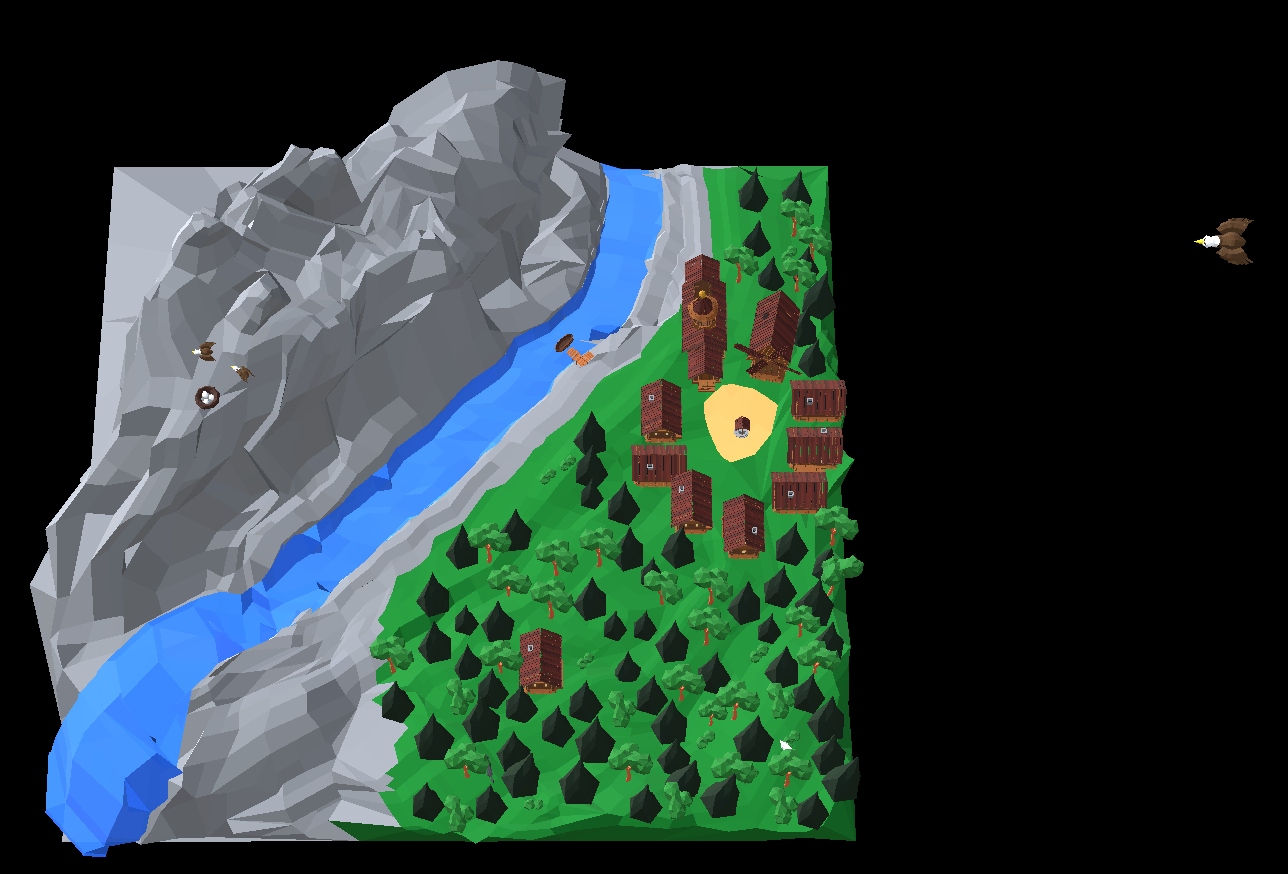
\includegraphics[width = 15cm, height = 8cm]{Komplette_welt_Draufsicht.png}
\caption{Hologramm der virtuellen Welt von oben}
Die Welt besteht aus einem Gebirge, einem Waldgebiet, einem Fluss und einem Dorf. In jedem Gebiet werden im Verlauf des Hörversuches virtuelle Schallquellen platziert.
\text{Rechts, über der Welt und dem Probanden, befindet sich zusätzlich ein weiterer Adler.}
\label{fig:Draufsicht}
\end{figure} 

\vspace*{40pt}
\subsection{Dorf}
Das Dorf befindet sich am Rand des Waldes und wird durch den Fluss vom Gebirge abgetrennt. Im Zentrum des Dorfes befindet sich ein Brunnen, der auf einer Sandfläche steht. Darum herum sind sieben einfache Häuser, sowie eine Mühle und eine Kirche platziert. Die Kirche besitzt einen Glockenturm mit einer goldenen Glocke. Diese könnte als potentielle virtuelle Schallquelle verwendet werden, wobei das Hörereignis der erschallenden Kirchenglocken ohne räumliches Audio wiedergegeben wird und somit keine Position in der Welt einnimmt. \\

 \begin{figure}[H]
\centering
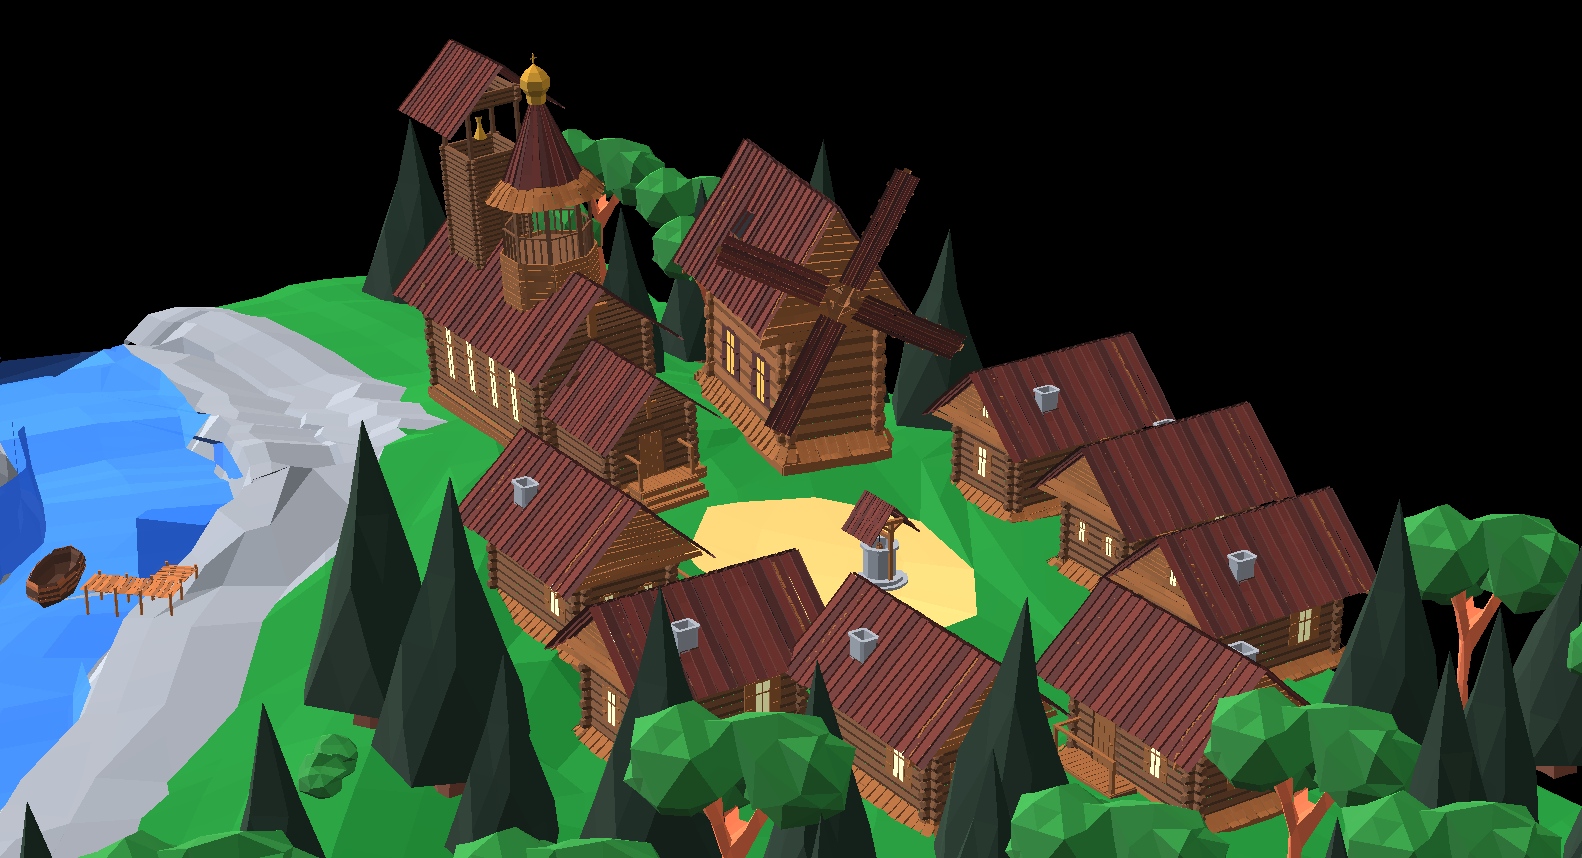
\includegraphics[width = 15cm, height = 8cm]{Dorf.png}
\caption{Dorf: Die Kirchenglocke dient als Ort für potentielle Schallquelle}
\label{fig:Dorf}
\end{figure} 

\subsection{Wald}
Der Wald besteht aus zum größten Teil aus Pflanzen und Bäumen. Im Wald befindet sich noch ein einfaches Haus und zwei Wölfe, wobei einer weiß und einer schwarz ist. Zu Beginn des Hörversuchs befindet sich der Wald im Vordergrund. Der weiße Wolf sticht hierbei durch seine Farbe, seine Größe und seine Position heraus, während der schwarze Wolf zunächst eher durch Bäume und Büsche verdeckt wird. Eine virtuelle Schallquelle wird an der Position des schwarzen Wolfes platziert. 

 \begin{figure}[H]
\centering
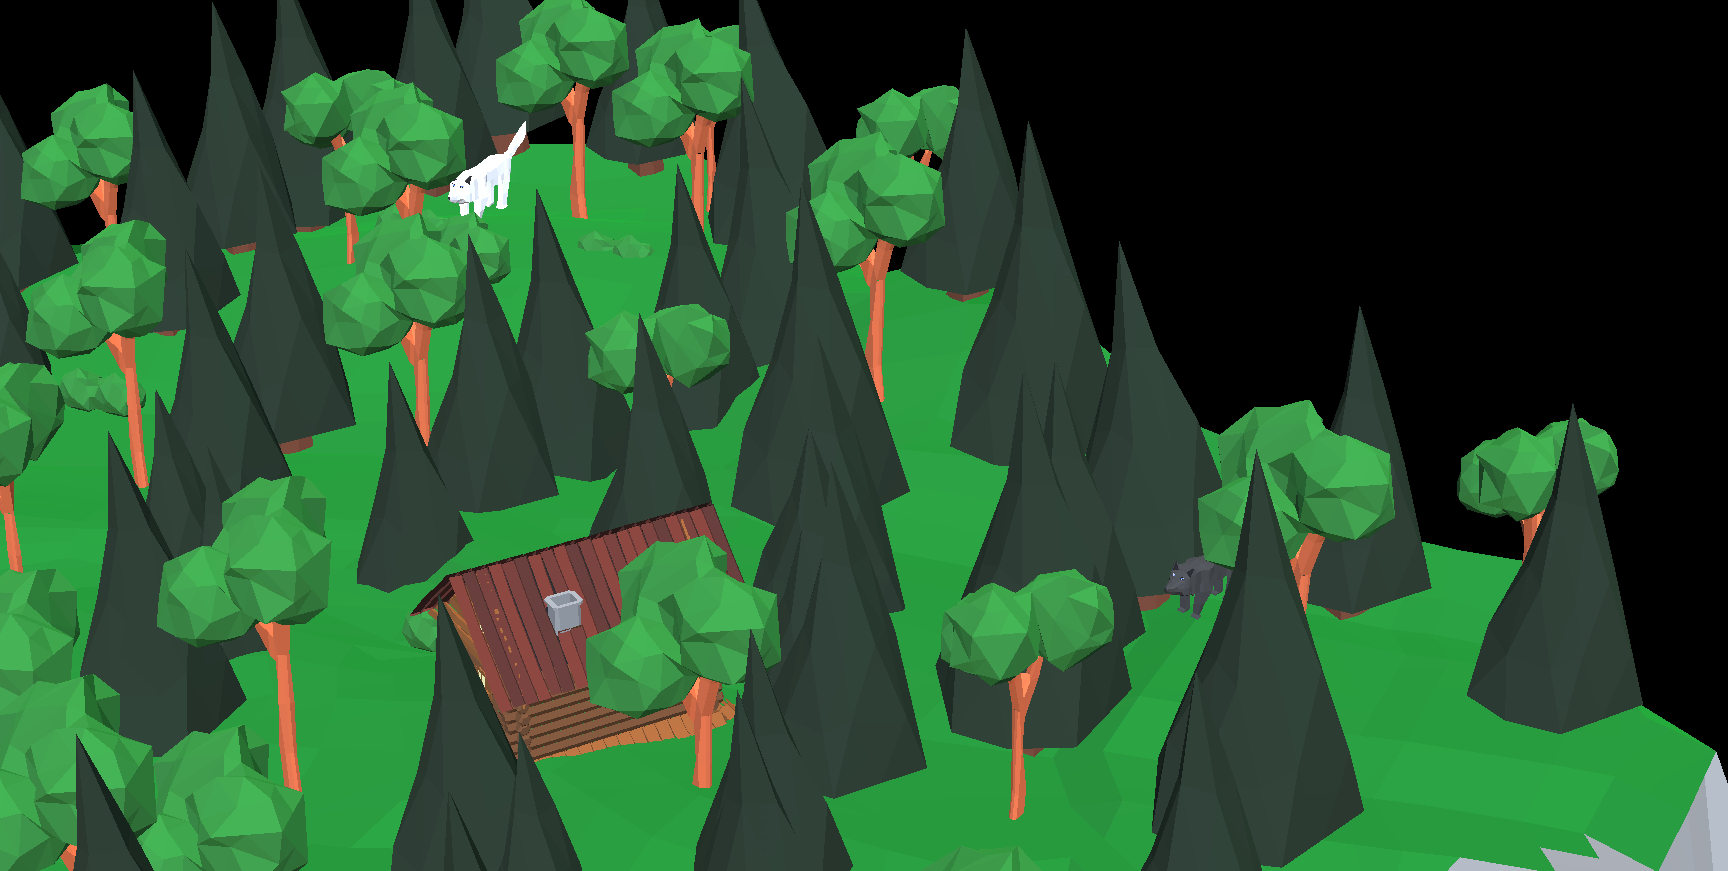
\includegraphics[width = 15cm, height = 8cm]{Wald.png}
\caption{Wald: Schwarzer Wolf dient als Ort für Schallquelle}
\label{fig:Wald}
\end{figure} 

\subsection{Gebirge und Fluss}
Das Gebirge ist das höchste Gebiet der Welt und wird vom Fluss von der restlichen Welt abgegrenzt. Die Bergspitze des größten Berges ist hierbei ca. 70cm hoch. In dem Gebirge befindet sich ein Adlernest, über dem zwei Adler fliegen. Eine virtuelle Schallquelle wird im Adlernest platziert. 

   Ein weiterer Adler befindet sich weit über der Welt, über dem Probanden. An dieser Position befindet sich ebenfalls eine virtuelle Schallquelle. Diese spielt das gleiche Signal ab, wie die virtuelle Schallquelle im Adlernest, siehe Abbildung \ref{fig:Draufsicht}. 

Am Fuße des Gebirges befindet sich ein Fluss. Dieser fließt von einer erhöhten Quelle abwärts in Richtung des Dorfes und geht hierbei von einem Kante der Karte bis zur gegenüberliegenden. 

An der Stelle, wo der Fluss an das Dorf angrenzt, befindet sich ein Steg mit einem kleinen Boot. Eine virtuelle Schallquelle wird an der Quelle des Flusses platziert und eine weitere im Boot. Beide virtuellen Schallquellen spielen das gleiche Audio-Signal ab. 

 \begin{figure}[H]
\centering
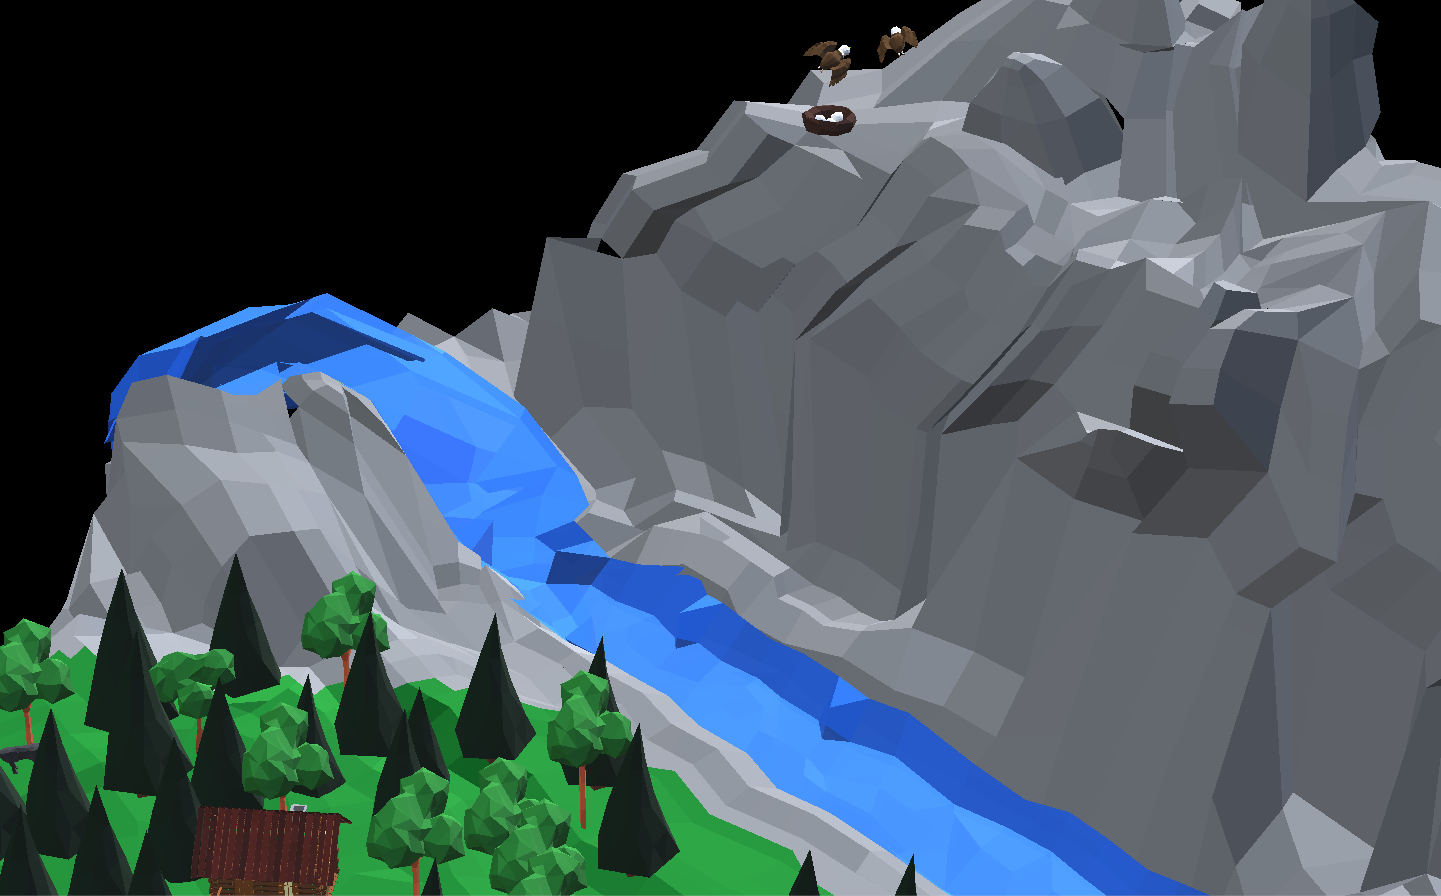
\includegraphics[width = 15cm, height = 8cm]{Gebirge_Fluss.png}
\caption{Gebirge und Fluss: Adler, Adlernest und Fluss dienen als  Ort für Schallquellen}
\label{fig:GebirgeFluss}
\end{figure}
   
  
   
\section{Audio-Einstellungen in der Applikation}
Die virtuelle Schallquelle ist in Unity ein Audio Source - Objekt. Die Einstellungen für das Audio Source Objekt sind nach dem Microsoft Tutorial für \glqq Spatial Audio\grqq für Mixed Reality vorgenommen worden \cite{MSSpatialAudio}. Diese Einstellungen gelten im Folgenden als Standart-Einstellungen. Abweichungen der Einstellungen werden in den Beschreibung für die Einzelszenen genannt.  Bei den abgespielten Audio-Signalen handelt es sich ausschließlich um MP3 codierte Geräusche die mit 48 kHz abgetastet werden. 
  
 
  \begin{figure}[H]
\centering
\includegraphics[width = 12 cm, height = 10 cm]{audio_Einstellungen.png}
\caption{Standarteinstellungen des \glqq Audio Source\grqq-Objektes in Unity}
Jede virtuelle Schallquelle in der Szene arbeitet mit genau diesen Einstellungen. \textbf{Spatial Blend} auf $1$ und die Aktivierung von \textbf{Spatialize} geben an, dass räumliches Audio, durch die digitale Faltung der Audio-Signale mit passenden, kopfbezogenen Übertragungsfunktionen, verwendet werden soll. 
\label{fig:audio_einstellungen}
\end{figure} 



\subsection{Binauralisierung in der Applikation}
   
Für das räumliche Audio wird der MS HRTF Spatializer und damit ein einheitlicher HRTF-Datensatz verwendet. Der MS HRTF Spatializer berechnet für die Szene jeweils die benötigten kopfbezogenen Übertragungsfunktionen für jedes Ohr des Probanden. Auf diese Weise gelingt eine räumliche, binaurale Wiedergabe der Audio-Signale über die Kopfhörer der HoloLens. 

\subsection{Auralisierung in der Applikation}

Für eine plausible Wiedergabe wird eine Anpassung der Geräusche an den Versuchsraum mittels Microsoft \glqq Spatial Audio\grqq vorgenommen. Hierfür wird ein abstraktes Raummodell des Versuchsraumes entworfen und in die Unity-Szene integriert \ref{fig:Raummodell}. Dem Raummodell wird anschließend ein "Audio Occluder"-Script hinzugefügt. Microsoft empfiehlt in seinem Tutorial bei den Parametern des "Audio Occluders" eine Tiefpass-Grenzfrequenz von 1500Hz und eine Lautstärkereduzierung um den Faktor 0.75 einzustellen, um plausiblen diffusen Nachhall zu imitieren\cite{MSSpatialAudio}.
 
  \begin{figure}[H]
\centering
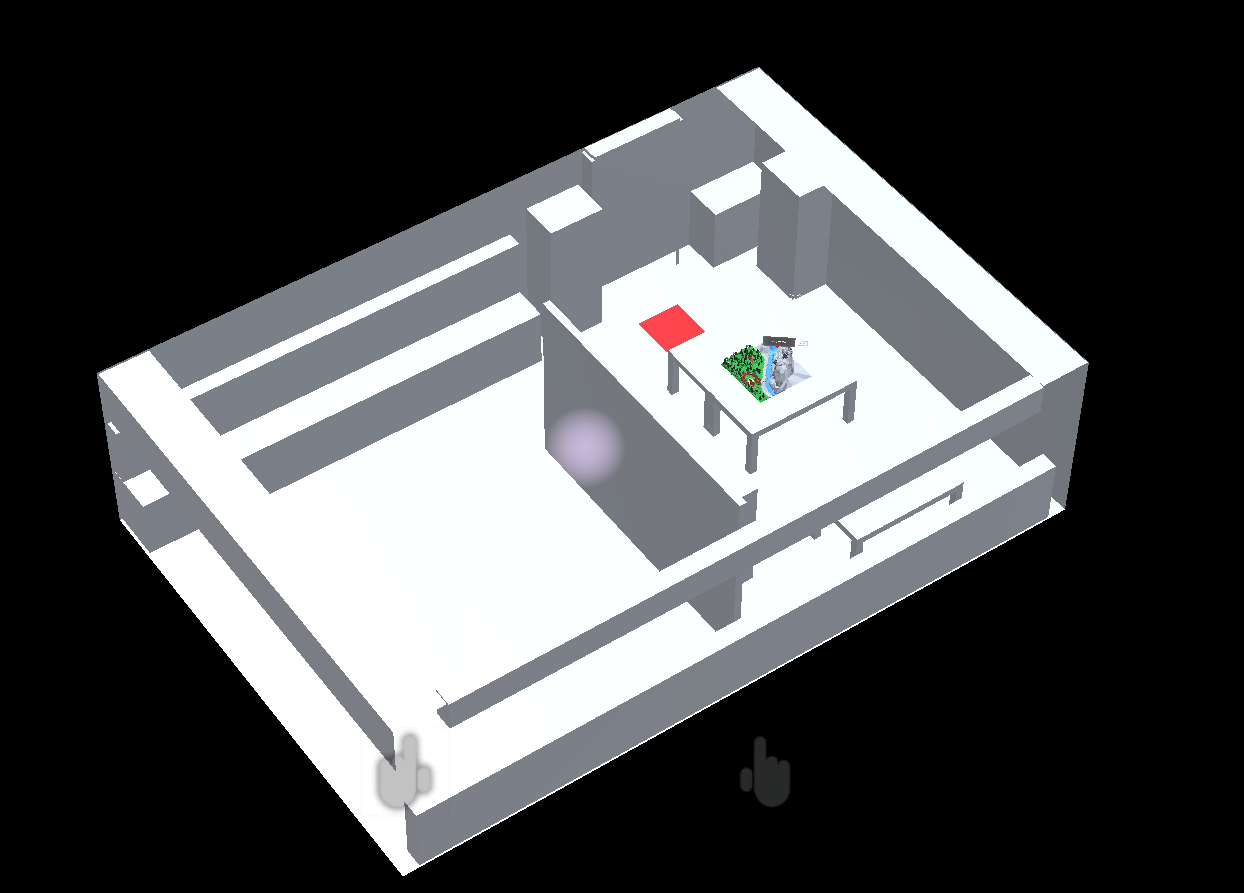
\includegraphics[width = 15cm, height = 8cm]{Raummodell_2.png}
\caption{Abstraktes Raummodell des Versuchsraumes E113 der HS Emden/Leer}
Das Raummodell mit Audio Occluder enthält die größten Objekte des Versuchsraumes und soll die Audio-Signale so beeinflussen, als ob das Geräusch wirklich aus dem Raum käme.
\label{fig:Raummodell}
\end{figure} 

Jedem Objekt mit einer Audio Source muss zusätzlich ein Audio Emitter zugewiesen werden. Die Parameter der Emitter werden wie folgt festgelegt: 

\begin{description}
\item[Update Intervall:] 0.15 
\item[Max Distance:] 20
\item[Max Objects:] 10
\end{description}

Durch die gewählten Parameter wird alle 0.15 Sekunden eine Neuberechnung der Raumakustik vorgenommen, was für die langsamen Bewegungen des menschlichen Kopfes genügen sollte.  Zusätzlich werden nur maximal 10 Objekte das Audio-Signal beeinflussen können. Diese dürfen dabei eine Distanz von maximal 20m entfernt sein. Mit diesen Einstellungen soll sichergestellt werden, dass die Anpassung der Audio-Signale einen natürlichen Klang hervorbringt. 

\vspace*{40pt}

  \section{Beschreibung der Szenen des Hörversuchs}
Der Hörversuch umfasst fünf verschiedene Szenen. In jeder Szene gibt es ein Hörereignis, das der Proband zu lokalisieren hat. Die Welt ist statisch und verändert sich während des Versuches nicht. Die virtuelle Schallquelle wird für jede Szene neu positioniert. 
\newpage
  \subsection{Szene 1: Adlerschrei im Gebirge}
  In der ersten Szene befindet sich die virtuelle Schallquelle im Adlernest, mitten im Gebirge. Bei dem Geräusch handelt es sich um das Schreien eines Adlers. Die Einstellungen weichen nicht vom gewählten Standard ab. 
  
    \begin{figure}[H]
\centering
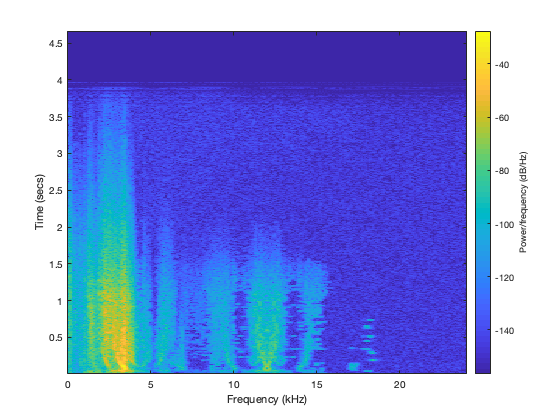
\includegraphics[width = 15cm, height = 10cm]{Adler_Spektogramm.png}
\caption{Spektorgramm des Adlerschreies}
Das Spektrogramm zeigt ein impulsartiges Geräusch im Bereich um 3 kHz, welches wenige Sekunden nachhallt. Die höheren Frequenzen über 7 kHz lassen dabei schneller nach als die intensiveren zwischen 2 kHz und 4 kHz. 
\label{fig:Adler_Spektogramm}
\end{figure} 

Abbildung \ref{fig:Adler_Spektogramm} zeigt das Spektogramm des Adlergeräusches. Es ist zu erkennen, dass das Geräusch ein breites Frequenzspektrum besitzt, jedoch die  Frequenzen zwischen 2 kHz und 4 kHz am intensivsten vertreten sind. Über den zeitlichen Verlauf lässt sich sagen, dass das Signal sich vor allem durch ein impulsartiges Geräusch am Anfang auszeichnet, dass im Frequenzbereich zwischen 2 kHz und 4 kHz noch einige Sekunden ausklingt, während die höheren Frequenzen schneller nachlassen.\\

 Der Schrei eines Adlers ist ein Geräusch, dass vermutlich jedem Probanden aus Fernsehen oder anderen Medien bekannt sein sollte. Gleichzeitig werden die meisten Probanden diesem Geräusch vermutlich noch nie in ihrem echten Leben begegnet sein. Das Geräusch ist wegen seines inhaltlichen Kontextes als eher unangenehm einzustufen. 

\newpage
\subsection{Szene 2: Wolfsheulen}

In der zweiten Szene befindet sich die virtuelle Schallquelle auf dem schwarzen Wolf im Wald. Das Geräusch beinhaltet das Heulen eines einsamen Wolfes. Das Spezielle an der Szene ist, dass es im unmittelbaren Blickfeld des Probanden eine alternative, potentielle Schallquelle mit dem weißen Wolf gibt. Dieser wird in der Regel vom Betrachter, aufgrund seiner Größe, seiner Erscheinung und seiner ungeschützten Position, leichter entdeckt. Interessant wird es daher zu beobachten, ob die Probanden in der Lage sind, auf Grund des Geräusches,  den schwarzen Wolf zu erblicken und diesen als virtuelle Schallquelle zu bestimmen.  Die Einstellungen für die Wiedergabe weichen erneut nicht vom gewählten Standard ab. 

 \begin{figure}[H]
\centering
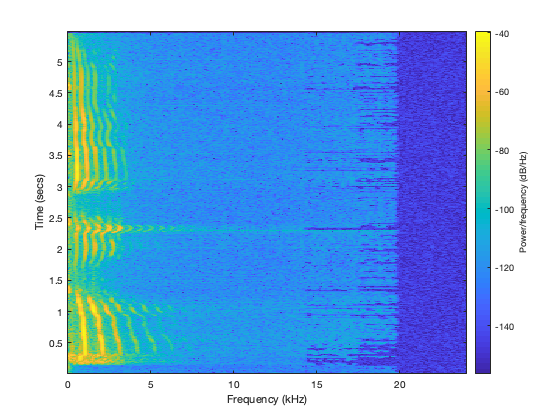
\includegraphics[width = 15cm, height = 10cm]{Wolf_Spektogramm.png}
\caption{Spektorgramm des Wolfsheulens}
Das Geräusch beinhaltet beinahe periodisch-vorkommende Töne bei ca.1 kHz und vielfachen der Frequenz bis 5 kHz. Es weist einen beinahe harmonischen Klang auf. 
\label{fig:Wolf_Spektogramm}
\end{figure} 

In Abbildung \ref{fig:Wolf_Spektogramm} ist das Spektogramm des Wolfsheulens zu sehen. Es ist zu erkennen, dass es sich in regelmäßigen, zeitlichen Intervallen auf ähnliche Art und Weise wiederholt. Das Geräusch besteht hauptsächlich aus Frequenzen zwischen 1 Hz und 5 kHz. Auffällig ist dabei, dass es zur Bildung schmaler Frequenzkeulen kommt, die sich bei vielfachen Frequenzen wiederholen. Es ist daher anzunehmen, dass sich das Geräusch harmonisch anhört. \\

Das Heulen eines Hundes könnte aufgrund der Verbundenheit des Menschen zu ihren Hunden ein Gefühl von Empathie auslösen. Wird das Geräusch eher als Wolfsheulen wahrgenommen, so könnte dieses Geräusch eher ein Angstgefühl beim Probanden bewirken. In beiden Fällen sollte das Geräusch ein befremdliches Gefühl auslösen und nicht als angenehm empfunden werden. 

\newpage
\subsection{Szene 3: Kirchenglocken}
Das Erklingen von Kirchenglocken in der dritten Szene wird ohne räumliches Audio durchgeführt und soll mit als Referenz dienen. Aus diesem Grund gibt es in dieser Szene keine virtuelle Schallquelle mit festgelegter Position. Es ist bei dieser Szene zu beobachten, ob die Probanden die Darbietung trotz des fehlenden, räumlichen Audios als plausibel und angenehm empfinden. Außerdem stellt sich die Frage, ob die Schallquelle, rein auf Grundlage der visualisierten Kirchenglocke, auch dort von den Probanden lokalisiert werden wird.
 
    \begin{figure}[H]
\centering
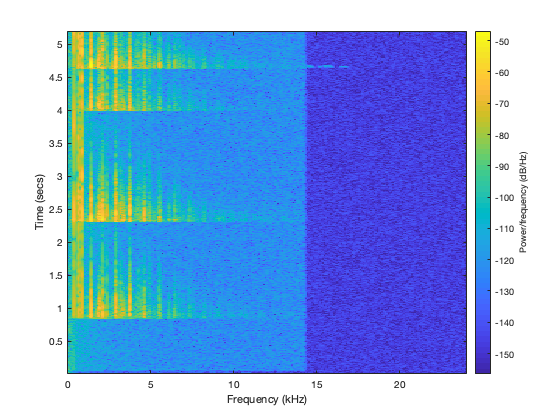
\includegraphics[width = 15cm, height = 10cm]{Kirchenglocken_Spektogramm.png}
\caption{Spektorgramm der Kirchenglocken}
Das Spektogramm zeigt einen sich wiederholenden Klang, aus Frequenzen zwischen 100 Hz und 10 kHz. Der Nachhall der tieferen Frequenzen klingt dabei nie vollständig ab. 
\label{fig:Kirchenglocken_Spektogramm}
\end{figure} 

Anhand Abbildung \ref{fig:Kirchenglocken_Spektogramm} lässt sich erkennen, dass das Geräusch der erklingenden Kirchenglocken ebenfalls eindeutige Frequenzkeulen aufweist, die sich bei vielfachen Frequenzen wiederholen. Aus diesem Grund handelt es sich ebenfalls um ein harmonisches Klangereignis. Das Frequenzspektrum umschließt Frequenzen zwischen 100 Hz und 10 kHz, wobei besonders die tiefen Frequenzen zwischen 100 Hz und 1 kHz sehr dominant sind. \\

Zeitlich verhält sich sich das Audio-Signal so, dass es immer zu einem  wiederholenden Anschlag der Glocken neu ertönt. Hierbei lassen die hohen  Frequenzen ebenfalls schneller nach als die tieferen. Besonders auffällig ist dabei, dass die sehr tiefen Grundtöne zwischen zwei Glockenschlägen nicht vollends abklingen, so dass diese Frequenzen dauerhaft zu hören sind.  \\

Das Erklingen von Glocken sollte in der Regel als angenehmes Geräusch wahrgenommen werden und wird häufig auch mit einem Friedensgefühl assoziiert. 
\newpage

\subsection{Szene 4: Adlerschrei über dem Probanden}
In der vierten Szene wird die virtuelle Schallquelle bei dem Adler über dem Probanden platziert. Das Geräusch ist hierbei das selbe wie bei der ersten Szene. \\ 

In der Realität handelt es sich bei dem Adlerschrei um ein Geräusch, dass eigentlich über dem Hörenden erwartet wird. Dadurch, dass sich das Geräusch nun tatsächlich über dem Probanden befindet, müsste es eigentlich ein plausibles Hörereignis darstellen. Es bleibt jedoch abzuwarten ob die Probanden anhand des Schalls den Adler über sich überhaupt lokalisieren können oder ob die offensichtlicheren Adler im Gebirge von der eigentlichen virtuellen Schallquelle ablenken.  

\vspace*{40pt}
\subsection{Szene 5: Flussrauschen}
In der letzten Szene  des Hörversuchs werden im Vergleich zu den anderen Szenen zwei virtuelle Schallquellen im Raum platziert, die beide das gleiche Geräusch wiedergeben. Bei diesem handelt es sich um das Rauschen eines Flusses. Eine virtuelle Schallquelle wird hierbei an der Quelle des Fluss, im Gebirge und eine neben dem Boot, am anderen Ende des Flusses platziert. Je nach Position des Probanden dürfte sich eine Phantomschallquelle entweder zwischen den beiden Schallquellen  oder an der nächstgelegenen Schallquelle bilden. 

 \begin{figure}[H]
\centering
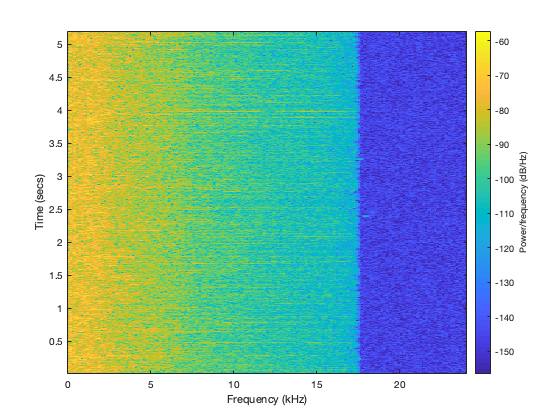
\includegraphics[width = 15cm, height = 10cm]{Fluss_Spektogramm.png}
\caption{Spektorgramm des Flussrauschens}
Das Spektogramm zeigt, dass das Flussrauschen einem rosa Rauschen sehr stark ähnelt. Durch die zeitliche Veränderung sollte dennoch kein durchgängig, gleich-klingendes Geräusch zu hören sein. 
\label{fig:Fluss_Spektogramm}
\end{figure} 

Das Spektogramm des Flussrauschens in Abbildung \ref{fig:Fluss_Spektogramm} ähnelt sehr dem eines rosa Rauschens. Von den tiefen zu den hohen Frequenzen nimmt die Intensität ab. Die beruhigende Wirkung von rosa Rauschen könnte dementsprechend  auch dem Flussrauschen zugesprochen werden. Trotz der Ähnlichkeit zum Rauschen verhält sich das Geräusch zeitweise unterschiedlich, so dass kein durchgängig, gleich-klingendes Geräusch wahrgenommen werden kann.  \\ 

Auch inhaltlich sollte das Rauschen eines Flusses eher als angenehm wahrgenommen werden. 
 \vspace*{20pt}
 \section{Bewertungskriterien der Darbietung}
 Zur Bewertung der Darbietung werden dem Probanden Fragen zum Darbietungsempfinden gestellt. Dieser hat der Proband mit Hilfe von jeweils  zwei dualistischen  Antwortmöglichkeiten zu beantworten. Dabei kann der Proband in zehn Stufen einordnen, welche der beiden Antworten für ihn eher zu trifft. Diese Art der Befragung erlaubt es den Probanden bei der Bewertung ihren Freiraum zu lassen, aber gleichzeitig die Probandendaten untereinander vergleichbar zu machen.  \\
 
 Mit Hilfe der Fragen soll herausgestellt werden, ob der Proband die Szene als plausibel wahrnimmt, inwiefern bei ihm ein Immersionsgefühl zustande kommt und ob er sich bei der Darbietung wohlgefühlt hat. \\
 
 Wird eine Szene als plausibel bezeichnet, dann bedeutet dies, dass die Summe aller Sinneseindrücke für den Betrachter glaubhaft und nachvollziehbar ist. Dies wird vor allem dann erreicht wenn die Sinneseindrücke natürlich wirken und den Konsumenten nicht verwirren. \\
 
 Ein wichtiges Kriterium für Plausibilität ist, dass die wichtigsten Sinneseindrücke, also das Gehörte und das Gesehene, zusammen passen. Ist beispielsweise ein Hörereignis ohne ersichtlichen Grund weit von der Schallquelle entfernt, dann widerspricht dies dem natürlich Verständnis des Menschen für Kausalität. Mit der ersten Frage soll daher geprüft werden, ob für den Probanden das Visuelle und das Auditive plausibel zusammenpassen.\\
 
 Ein weiteres Kriterium Plausibilität ist der Realismus der Sinneseindrücke. Hierbei geht es weniger darum, dass visuelle und auditive Reize als komplett realistisch wahrgenommen werden, sondern vielmehr darum, dass diese sich in das Gesamtbild einfügen. Da das Visuelle in dem Hörversuch auf einem Low-Poly-Grafikstil basiert, wird niemand von den Geräuschen absoluten Realismus erwarten. Wichtig ist jedoch trotzdem, dass die Geräusche als Komponente der unmittelbaren Umgebung wahrgenommen werden, anstatt als alleinstehendes Audio-Signal, welches über die Kopfhörer wiedergegeben wird. Die zweite Frage soll daher Klarheit darüber geben, inwiefern die Probanden die Geräusche als realen Bestandteil ihrer Umgebung wahrnehmen. \\
 
 \newpage
Bei der Erstellung von AR- und VR-Anwendungen ist das Wohlbefinden des Konsumenten ein zu beachtender Faktor. Das stärkere Immersionsgefühl bei AR und VR ermöglicht es noch realistischere, mediale Inhalte zu erstellen. Dies setzt aber auch voraus, darauf zu achten unter welchen Umständen sich der Konsument wohlfühlt. Mit der Entdeckung des Uncanny Valley wurde bereits bewiesen, dass zu realistische visuelle Reize Unwohlsein auslösen können. Inwiefern dies auch mit dem steigernden Realismus von räumlichem Audio bewirkt werden könnte ist noch nicht vollends erforscht. Aus diesem Grund soll mit der dritten Frage das Wohlbefinden des Probanden während der Darbietung überprüft werden. 
 
 \vspace*{20pt}
 \begin{figure}[H]
\centering
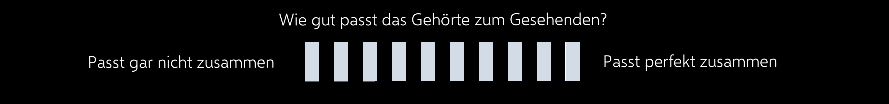
\includegraphics[width = 16cm, height = 2cm]{Frage1.png}
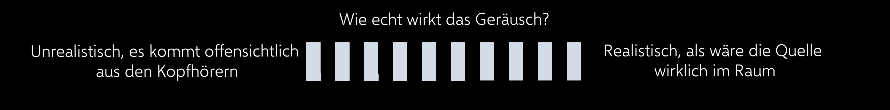
\includegraphics[width = 16cm, height = 2cm]{Frage2.png}
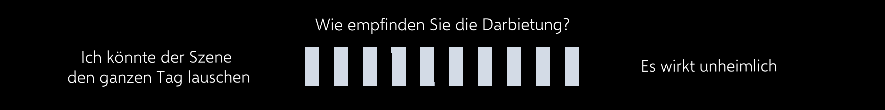
\includegraphics[width = 16cm, height = 2cm]{Frage3.png}
\caption{Fragen zur Bewertung der Szenen im Hörversuch}
Mit Hilfe der Fragen soll ermittelt werden, wie plausibel der Proband die räumliche Audio-Wiedergabe und die Szene findet und wie wohl er sich bei der Darbietung fühlt.
\label{fig:Fragen}
\end{figure} 
 \vspace*{10pt}

Anhand der Bewertungen des Probanden soll ermittelt werden, wie stark das Immersionsgefühl bei der Darbietung der Szenen gewesen ist. Nimmt ein Proband das Geräusch als Teil des Raumes war, empfindet gleichzeitig das Zusammenspiel aus Visuellem und Auditivem als plausibel und fühlt sich dann noch wohl bei der Darbietung, dann ist auch davon auszugehen, dass das Immersionsgefühl des Probanden recht intensiv ist. Auf diese Weise soll überprüft werden bei welcher Szene das stärkste Immersionsgefühl bewirkt wird. \\ 

Die zu Anfang gestellte These, dass es eine Art Uncanny-Valley-Effekt für zu realistisches, räumliches Audio geben könnte, soll anhand der Versuchsergebnisse ebenfalls überprüft werden. Lässt sich ein Zusammenhang zwischen dem dem bewerteten Realismus der Szene aus Frage 2 und dem geprüften Wohlbefinden aus Frage 3 beobachten, dann könnte dies Aufschluss über die gestellte These geben. Natürlich sind die durchgeführten Versuche für die Bestätigung der These nicht vollends aussagekräftig, da der Hörversuch nicht ausschließlich auf die Erforschung dieses Themengebietes ausgelegt ist. 
 
 \newpage
 \section{Beschreibung der Benutzeroberfläche}
 Die Bedienung der HoloLens-App funktioniert über Head-Tracking, Gesten- und Sprachsteuerung, wobei die Probanden für den Hörversuch ausschließlich auf die Head-Tracking-Funktion und die Gestensteuerung zurückgreifen mussten. \\
 
 Mittels eines Cursors, der wie eine Computermaus funktioniert, lassen sich in der App Aktionen durchführen. Der Cursor befindet sich hierbei immer in der Mitte des Sichtfeldes des HoloLens-Nutzers. Über die Bewegung des Kopfes kann der Benutzer nun den Cursor bewegen. Der Cursor besitzt drei Darstellungsformen, um dem Nutzer seinen aktuellen Zustand zu signalisieren, siehe Abbildung \ref{fig:Cursor}. 
 
  \begin{figure}[H]
\centering
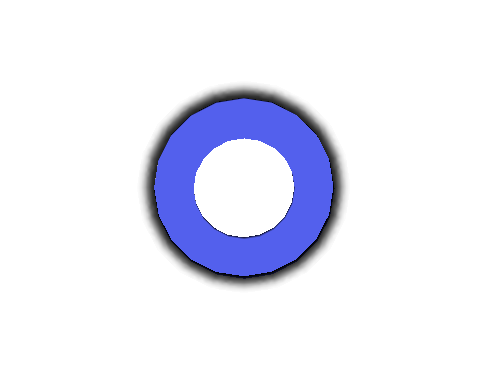
\includegraphics[width = 5cm, height = 4cm]{Cursor_default.png}
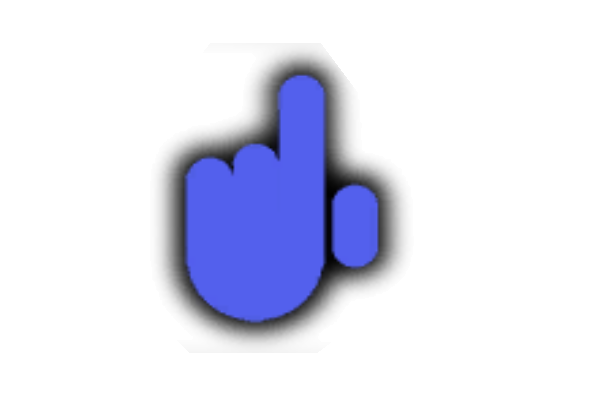
\includegraphics[width = 5cm, height = 4cm]{Cursor_Hand_Erkannt.png}
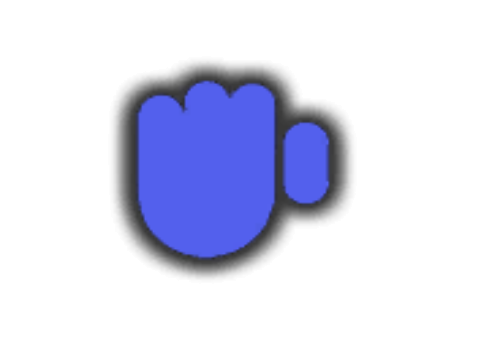
\includegraphics[width = 5cm, height = 4cm]{Cursor_Tap_Erkannt.png}
\caption{Mögliche Cursor-Zustände in der App}
Es gibt drei verschiedene Cursor-Zustände. Wird ein Hologramm anvisiert und keine Hand erkennt, dann wird der Default-Cursor(links) verwendet. Wird die Hand des Benutzers erkannt, dann wird der mittlere Cursor-Zustand angezeigt. Bei Durchführung der Tap-Geste signalisiert der rechte Cursor-Zustand die erfolgreiche Ausführung des Taps. 
\label{fig:Cursor}
\end{figure} 
 
  \vspace*{20pt}
 Der Cursor lässt sich über Handgesten steuern. Hebt man die Hand vor sich hoch, so dass die Sensoren der HoloLens diese erkennen können, dann verändert sich der Cursor in eine Hand, siehe Abbildung \ref{fig:Cursor}. Hebt man von der geschlossen Hand aus den Zeigenfinger und drückt diesen ruckartig wieder nach unten, wird dies als Tap-Geste bezeichnet. Wurde die Tap-Geste erfolgreich von der HoloLens erkannt, dann verändert sich der Cursor erneut, siehe \ref{fig:Cursor}. Die Tap-Geste ist ein Mittel um mit Objekten in der virtuellen Welt zu interagieren. \\
 
 Auch die Beantwortung der Fragen zur Bewertung der Darbietung gelingt über die Tap-Geste. In dem der Proband auf einen der Balken zwischen den Antwortmöglichkeiten klickt kann dieser die Szene bewerten.
 
  \begin{figure}[H]
\centering
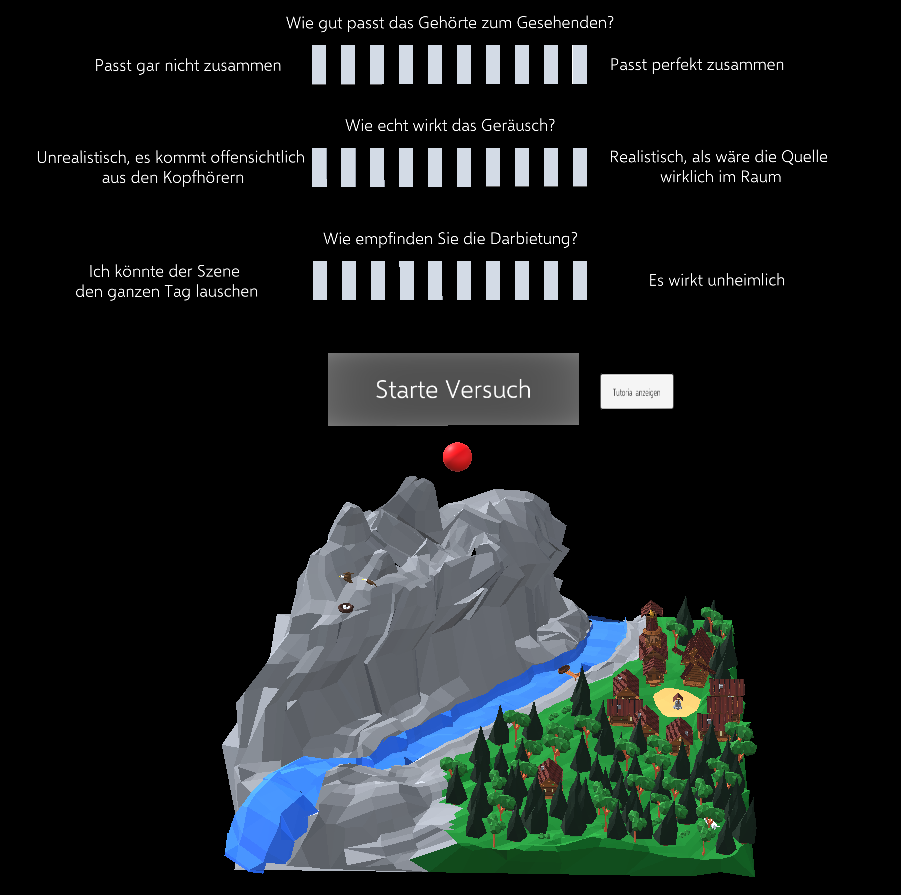
\includegraphics[width = 13cm, height = 14cm]{Welt_mit_Interface.png}
\caption{Virtuelle Welt mit Benutzeroberfläche und roter Kugel}
Die virtuelle Welt wird zusammen mit der Benutzeroberfläche in dieser Form auf den Tisch vor den Probanden projiziert. Mit Hilfe der roten Kugel lässt sich vom Probanden die Position der lokalisierten Schallquelle angeben. Mit den Balken unter den Fragen lässt sich diese gewichtet beantworten. 
\label{fig:WeltMitInterface}
\end{figure} 
 \vspace*{10pt}
 
 \subsubsection{Position der Schallquelle lokalisieren}
 Eine Aufgabe des Probanden im Hörversuch ist es die Position der virtuellen Schallquelle zu lokalisieren. Damit dies spielerisch gelingt hat der Proband in der HoloLens-App die Möglichkeit eine rote Kugel dort zu platzieren, wo er denkt, dass sich die virtuelle Schallquelle befindet. Die rote Kugel befindet sich am Anfang jeder Szene direkt über der virtuellen Welt, siehe Abbildung \ref{WeltMitInterface}. Der Proband hat nun die Möglichkeit die Kugel mit dem Cursor anzuvisieren und mit der Tap-Geste die Kontrolle über die rote Kugel zu erhalten. Hat er die vermeintliche Position der virtuellen Schallquelle lokalisiert, kann er mit Hilfe von Kopfbewegung die rote Kugel dorthin bewegen und mit einer weiteren Tap-Geste an der gewünschten Position platzieren. So kann der Proband leicht und sofort visualisiert angeben, wo er die Schallquelle hört. 
 
 \subsubsection{Sprachbefehle und Positionierung der Welt}
 Für die Positionierung der Welt wurden Sprachbefehle implementiert mit denen sich die Welt bewegen lässt. Mit dem Start der App befindet sich die Welt im Rotationsmodus (Sprachbefehl: \glqq Rotate Mode\grqq), wodurch sich die Welt mit der Tap-Geste um die Y-Achse rotieren lässt. Mit dem Sprachbefehl \glqq Move Mode\grqq wird in den Bewegungsmodus gewechselt. In diesem lässt sich die Welt frei im Raum bewegen. Ist die gewünschte Rotation und Transformation eingestellt, so lässt sich mit dem \glqq Lock Mode\grqq -Sprachbefehl die Welt feststellen. Die Hörversuche sollten im \glqq Lock Mode\grqq durchgeführt werden, damit der Proband nicht fälschlicherweise die Welt während des Hörversuchs bewegt. Die Sprachbefehle werden den Probanden nicht beigebracht und dienen ausschließlich zur Kontrolle über die Welt.
  
\vspace*{180pt}
 \section{Ablauf des Hörversuchs}
 Zu aller erst wird die App auf der HoloLens im Versuchslabor gestartet. Wichtig dabei ist, dass beim Start der App der Träger der HoloLens sich an der durch das Raummodell festgelegten Stelle befindet. Nur dann stimmt das in Unity festgelegte Raummodell mit dem realen Versuchsraum überein, so dass ein plausibles akustisches Ergebnis durch Spatial Audio erzielt werden kann. \\
 
 Im Anschluss wird das Hologramm der Welt, mit Hilfe der Sprachbefehle, auf dem dafür vorgesehenen Tisch platziert und festgestellt. Daraufhin kann die HoloLens an den ersten Probanden übergeben werden. \\
 
Zu Beginn des Hörversuchs stellt sich jeder Proband zunächst an die vorgesehene Stelle im Raum. Damit die Ergebnisse des Hörversuchs nicht durch eine variierende Wortwahl bei der Erklärung verfälscht werden, erhalten alle Probanden die gleiche Einweisung über ein Tutorial-Fenster, welches über die HoloLens dargeboten wird.  \\

 \begin{figure}[H]
\centering
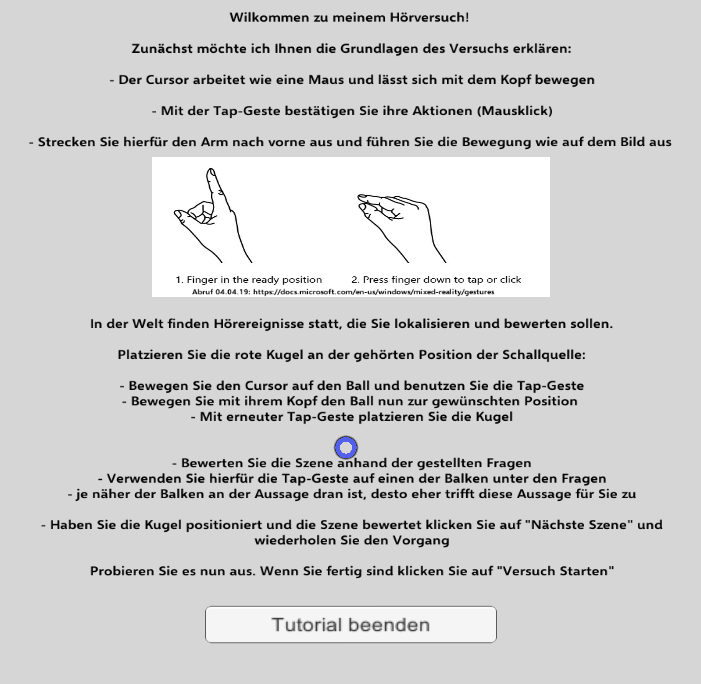
\includegraphics[width = 13cm, height = 13cm]{Tutorial.png}
\caption{Einheitliches Tutorial für die Probanden zur Erklärung der Steuerung im Hörversuch}
\label{fig:Tutorial}
\end{figure} 

Sind nach der Einweisung noch Fragen offen, so kann der Proband diese vor dem Beginn des Hörversuchs klären. Mit dem Beenden des Tutorials sieht der Proband die Welt wie in Abbildung \ref{fig:WeltMitInterface}. Hier kann der Proband testen, ob er das Tutorial verstanden hat und sowohl die Balken der Fragen markieren, als auch die Kugel im Raum platzieren.  \\
 
 Hat der Proband alles verinnerlicht ist er bereit den Hörversuch über den "Versuch starten"-Button zu starten. Daraufhin sollte das Geräusch der ersten Szene abgespielt werden. Die Aufgabe des Probanden ist es nun die rote Kugel an der Stelle zu platzieren, an der er die virtuelle Schallquelle hört und anschließend die Fragen über der Welt zu beantworten. Ist dies erledigt kann der Benutzer mit dem "Nächste Szene"-Button die nächste Szene laden. Dieser Vorgang wiederholt sich für alle fünf Szenen. Mit dem Beendigen der fünften Szene wird dem Probanden über ein Pop-Up-Fenster signalisiert, dass der Versuch abgeschlossen ist. \\
 
 Die Daten des Probanden werden für jede Szene  einzeln, lokal auf der HoloLens in einer Text-Datei gespeichert. Hierbei werden die zur Welt relativen Koordinaten und die Bewertungen als Zahlen von -5 bis 5 gespeichert. 
 
 
 \section{Probanden}
 
 Bei den für den Hörversuch ausgewählten Probanden handelt es sich hauptsächlich um Studierende der Hochschule Emden/Leer. Der Hörversuch wurde hierbei mit 17 unterschiedlichen Probanden durchgeführt, wobei leider einige aus Zeitgründen nicht alle Szenen des Versuchs durchführen konnten und vereinzelnd Probandendaten aufgrund von Bugs der App verloren gegangen sind. \\
 
  Das Alter der Probanden lag hierbei zwischen 20 und 50 Jahren, wobei die meisten zwischen 20 und 30 Jahren alt waren. Anzumerken ist hierbei, dass die abgespielten Geräusch aller eher niederfrequent waren und daher eine Beeinflussung der Ergebnisse durch das Alter in der Auswertung vernachlässigt wird. \\ 
  
 Zwölf der getesteten Personen waren männlich und drei  weiblich . Einige Probanden trugen unter der HoloLens eine Brille, dies soll aber bei der Auswertung trotz des möglichen Einflusses auf die Ergebnisse nicht weiter berücksichtigt werden. \\ 
 
 Der Hörversuch erfolgte anonym und ohne Erfassung persönlicher Daten. Die Auswertung der Probandendaten erfolgt ohne Hintergrundinformationen über die Probanden und basiert ausschließlich auf den durch die App gespeicherten Daten. Für sicherere Versuchsergebnisse sollte der Hörversuch mit einer größeren Menge an Probanden, sowie einer Erfassung der persönlichen Probandendaten, wiederholt werden.
 
 \chapter{Auswertung des Hörversuchs}
 Im Rahmen dieser Bachelorarbeit wurde ein Hörversuch mit binauralem, räumlichem Audio durchgeführt. Ziel des Hörversuches war es herauszufinden, inwiefern die natürliche Lokalisationsfähigkeit von Hörereignissen in einer Mixed Reality Umgebung gegeben ist. Bei der Durchführung des Hörversuches haben die Probanden, für fünf verschiedene Audio-Szenen, jeweils versucht virtuelle Schallquellen zu lokalisieren.  Zusätzlich haben sie zu jeder Szene Fragen zum Darbietungsempfinden, anhand bestimmter Kriterien, beantwortet.  Die Ergebnisse des durchgeführten Hörversuches sollen im Folgenden analysiert werden.
 
 \section{Versuchsergebnisse}
 Während des Versuchs hatten die Probanden für jede Szene die Aufgabe eine rote Kugel genau dort zu platzieren, wo sie die virtuelle Schallquelle anhand des Gehörten vermuteten. Die Position der roten Kugel wurde hierbei für jeden Probanden, für jede Szene dokumentiert. Es gilt nun die gesammelten Daten zu analysieren. \\
 
 Zur Visualisierung der Ergebnisse wird die virtuelle Welt zusammen mit der wirklichen, virtuellen Schallquelle und den von den Probanden lokalisierten, virtuellen Schallquellen dargestellt. Die echte, virtuelle Schallquelle wird, sofern es eine gibt, durch eine rosa Kugel und die von den Probanden lokalisierte virtuelle Schallquelle durch kleinere, rote Kugeln dargestellt. Hierbei ist anzumerken, dass die Platzierung der roten Kugel, aufgrund fehlender Übung mit dem Umgang der HoloLens, nicht komplett genau erfolgen konnte. Es sollte daher bei der Analyse berücksichtigt werden, dass die Probanden die Kugel vielleicht nicht genau da platzieren konnten, wo sie die Schallquelle ganz genau gehört haben. 
 
 \subsection{Szene 1: Adlerschrei im Gebirge}
 In der ersten Szene wurden die in den Microsoft-Tutorials für Spatial Audio empfohlenen Einstellungen für räumliches Audio direkt übernommen. Die virtuelle Schallquelle mit dem Schrei eines Adlers wurde für die Szene direkt in das Adlernest gelegt. Anhand der Abbildung \ref{fig:Szene_1_data} lässt sich erkennen, dass die Probanden die virtuelle Schallquelle fast ausnahmslos auf der Oberfläche des Berges, neben dem fliegenden Adler lokalisiert haben. Es ist anzunehmen, dass die Probanden versucht haben die Kugel genau auf dem Adler zu platzieren und nicht im Nest, wie vorgesehen. Einige Schallquellen wurden außerdem weiter rechts im Gebirge und auch einige über dem Gebirge lokalisiert. In Abbildung \ref{fig:Szene_1_data_2} ist zu sehen, dass ein Proband die Schallquelle, sogar weit über sich, beim dritten Adler lokalisiert hat. 
 
   \begin{figure}[H]
\centering
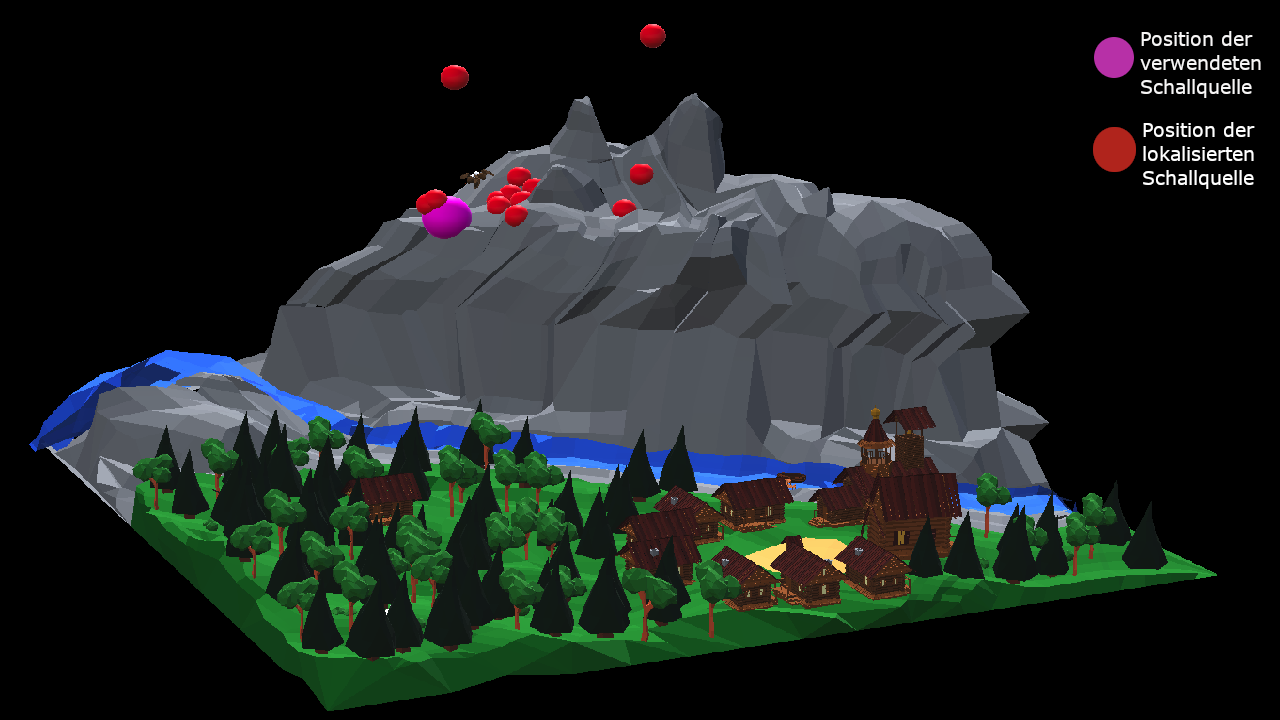
\includegraphics[width = 16cm, height = 9cm]{Szene_1_data.png}
\caption{Visualisierung der lokalisierten, virtuellen Schallquellen für Szene 1}
Die meisten Probanden haben die virtuelle Schallquelle beim Adler lokalisiert. 
\label{fig:Szene_1_data}
\end{figure} 

\begin{figure}[H]
\begin{minipage}[t]{7cm}
\vspace{0pt}
\centering
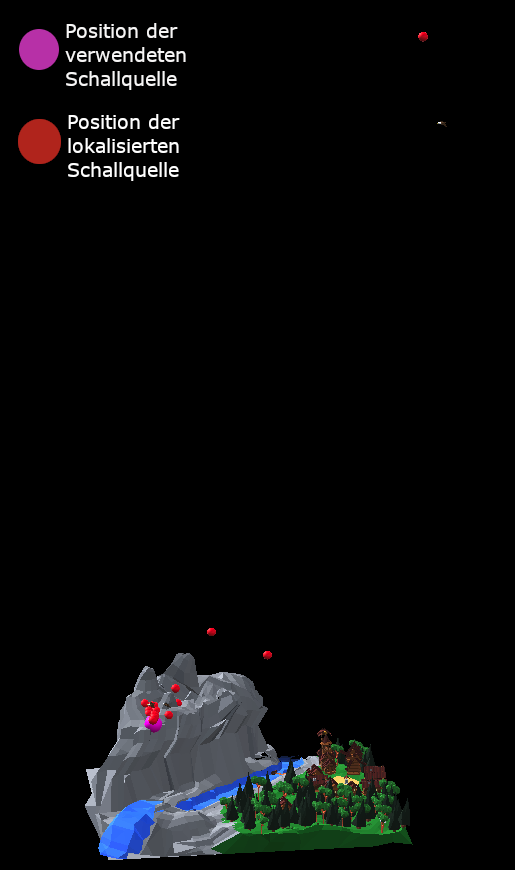
\includegraphics[width = 5cm, height = 9cm]{Szene_1_data_2.png}
\caption{Visualisierung der lokalisierten, virtuellen Schallquellen für Szene 1 aus der Seitensansicht}
\label{fig:Szene_1_data_2}
\end{minipage}
\hfill
\begin{minipage}[t]{9.5cm}

Anhand der Lokalisationen lässt sich erschließen, dass die Probanden zum größten Teil die ungefähre Position der virtuellen Schallquelle hören konnten. Das Wissen, dass in Wirklichkeit die Schallquelle direkt auf dem Adler liegen müsste, ließ die meisten Probanden die virtuelle Schallquelle jedoch direkt auf dem Adler vermuten. Anzumerken ist jedoch, dass auch einige die Schallquelle genau richtig im Nest platziert haben, obwohl dies nicht direkt zum inhaltlichen Kontext passt. \\

Es ist ebenfalls festzuhalten, dass bis auf drei Probanden alle die virtuelle Schallquelle in der gleichen Höhe lokalisiert haben. Die Verteilung in der Horizontaltebene ist hingegen breiter gestreut. \\

Die Platzierung der Schallquelle über dem Probanden könnte ein Indiz dafür sein, dass das Visuelle einen höheren Einfluss auf die Lokalisation der Hörereignisse hat als gedacht. Obwohl der Schall eigentlich nicht so klingen sollte, als ob er von oben käme hat der Proband die Schallquelle trotzdem dort lokalisiert. Jedoch sollte berücksichtigt werden, dass es sich hierbei um einen einzelnen Ausreißer handelt.
\end{minipage}
\end{figure}


   \begin{figure}[H]
\centering
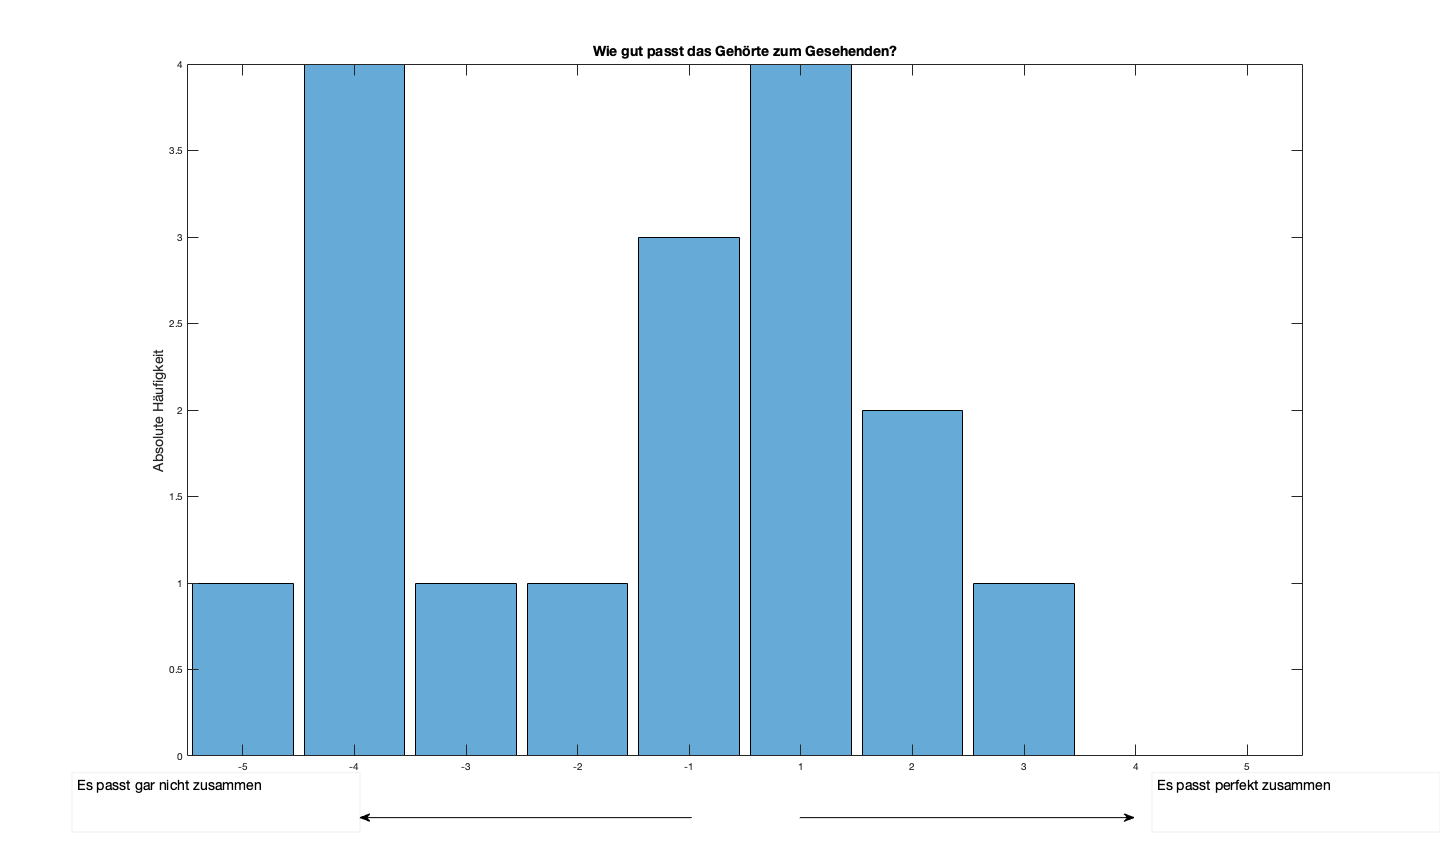
\includegraphics[width = 18cm, height = 10cm]{Szene_1_Frage_1.png}
\caption{Histogramm: Wie gut passen Visuelles und Auditives in Szene 1 zusammen?}
Für die meisten Probanden hat keine der Aussagen wirklich gut gepasst. Trotzdem waren mehr Probanden dafür, dass Visuelles und Auditives nicht zusammengepasst haben. 
\label{fig:Szene_1_Frage1}
\end{figure} 

\vspace*{30pt}

Bei der Beurteilung, ob Visuelles und Auditives zusammen passen waren die Meinungen sehr unterschiedlich, siehe Abbildung \ref{fig:Szene_1_Frage1}. Wohingegen sieben Probanden die visuelle und auditive  Darbietung als wenig bis gar nicht als zusammenpassend empfunden haben, haben nur für drei Probanden diese halbwegs zusammengepasst. Damit kann für die erste Szene festgehalten werden, dass die auditiven und visuellen Inhalte eher geringfügig zusammenpassen. \\

Grund für die eher suboptimale Darbietung könnte unter anderem sein, dass die virtuelle Schallquelle nicht auf dem Adler sondern im Adlernest liegt und daher das gehörte Geräusch nicht zur Position des Adlers passt. Allerdings könnte das Geräusch auch an sich als unpassend zum 3D-Modell des Adlers bewertet werden. Des Weiteren muss immer beachtet werden, dass das Visuelle statisch ist, während das Auditive sich zeitlich verändert. \\ 


   \begin{figure}[H]
\centering
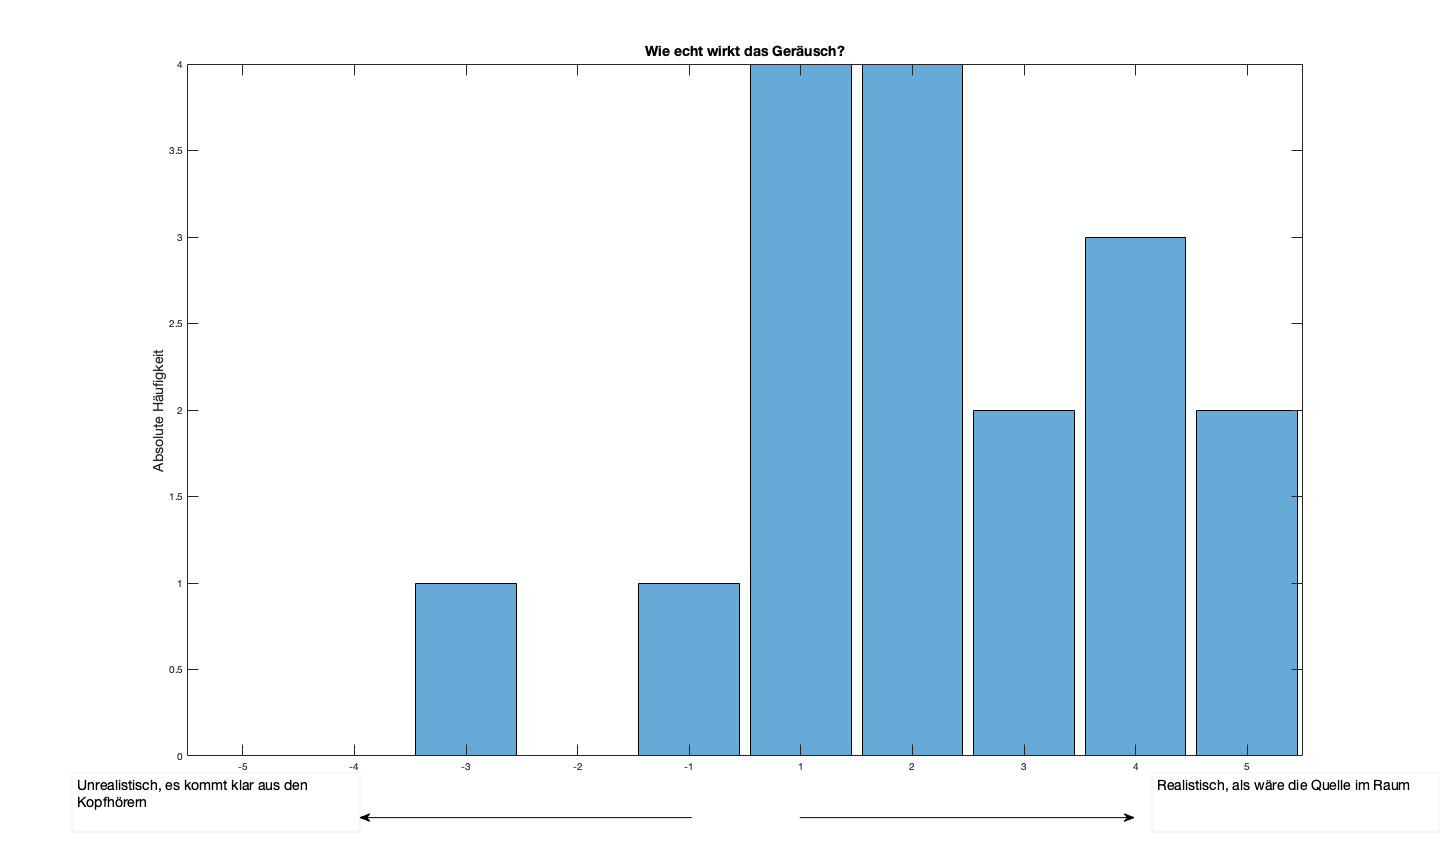
\includegraphics[width = 18cm, height = 10cm]{Szene_1_Frage_2.png}
\caption{Histogramm: Wie echt wirkt das Geräusch im Raum in Szene 1?}
Der Großteil der Probanden bewertet das Geräusch als plausibles Hörereignis im Raum, während für einige das Hörereignis weder realistisch, noch unrealistisch klingt.
\label{fig:Szene_1_Frage2}
\end{figure} 
\vspace*{30pt}

Anhand der Abbildung \ref{fig:Szene_1_Frage2} lässt sich deuten, dass das Geräusch wirklich als Bestandteil des Raumes wahrgenommen wird. Für nur zwei Probanden wirkt das Geräusche als halbwegs unrealistisch, während es für alle anderen Probanden als halbwegs realistische bis komplett realistische Quelle im Raum wahrgenommen wird. Es kann für die erste Szene daher von einer erfolgreichen Auralisierung gesprochen werden, bei der die Schallquelle wirklich als plausibler Bestandteil des Raumes wahrgenommen werden kann. 

\begin{figure}[H]
\centering
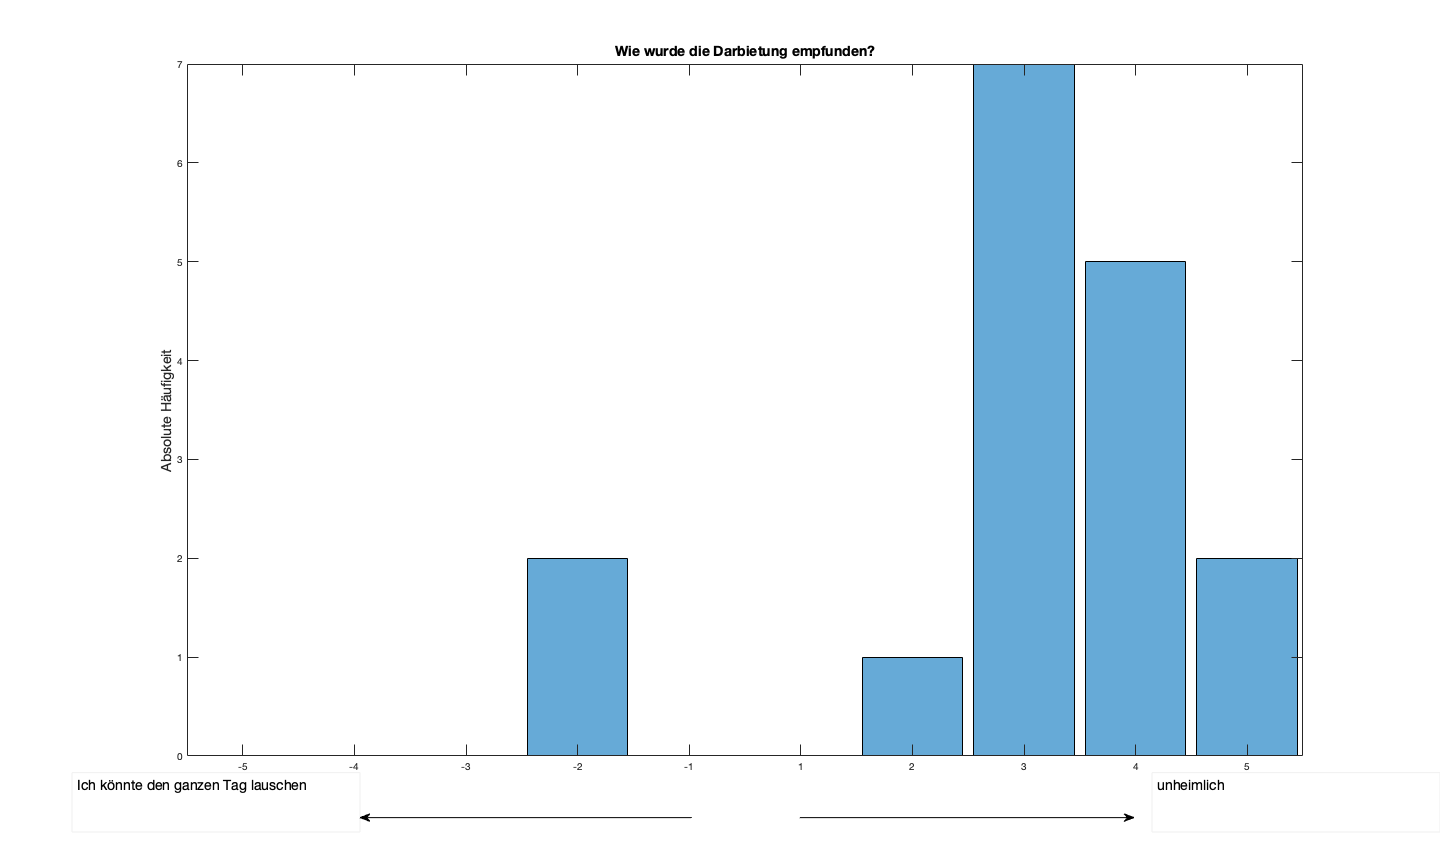
\includegraphics[width = 18cm, height = 10cm]{Szene_1_Frage_3.png}
\caption{Histogramm: Wie angenehm war die Darbietung von Szene 1?}
Die Darbietung wurde als äußerst unheimlich bewertet. Nur zwei Probanden empfanden sie als halbwegs angenehm. 
\label{fig:Szene_1_Frage3}
\end{figure} 


Abbildung \ref{fig:Szene_1_Frage3} zeigt eindeutig, dass die Darbietung von fast allen Probanden als unheimlich empfunden worden ist. 14 der 16 Probanden haben dabei die Darbietung mit drei oder höher auf der \glqq Unheimlichkeits\grqq{}-Skala bewertet. Die Darbietung scheint, wie es die Bewertungen erkennen lassen, wirklich unheimlich bei den Probanden angekommen zu sein.\\

Vereint man diese Erkenntnis mit den Ergebnisse aus Abbildung \ref{fig:Szene_1_Frage2}, dann bekräftigt das empfundene Unbehagen der Probanden die These eines \glqq Uncanny-Valley\grqq{}-Effekts für realistisches, räumliches Audio. Die Schallquelle wird größtenteils als realistische Quelle im Raum wahrgenommen und gleichzeitig wird bei fast allen Probanden durch die Darbietung Unbehagen ausgelöst. Dieser Aspekt soll auch in den folgenden Szene noch weiter beobachtet werden. \\

Anzumerken ist jedoch, dass das Geräusch an sich auch schon die unheimliche Stimmung der Szene bewirken könnte, da der Schrei eines Raubtieres in der Regel immer mit einer Form der Bedrohung verbunden wird, auch wenn der Adler an sich kein natürlicher Fein des Menschen ist. 

Anhand der Ergebnisse der Fragen lässt sich schwer eine Aussage über das Immersionsempfinden der Probanden aufstellen. Die weitläufige Verteilung der Antworten auf die Frage, ob Visuelles und Auditives als zusammenpassend wahrgenommen werden lässt vermuten, dass die Probanden auch unterschiedlich stark in die virtuelle Welt eintauchen konnten. Besonders die Tatsache, dass die Szene fast ausnahmslos als unheimlich empfunden worden ist, könnte, trotz der empfundenen Echtheit der Schallquelle im Raum, eine Immersion der Probanden in die erweiterte Realität verhindert haben. \\

 \subsection{Szene 2: Wolfsheulen}
 Bei der zweiten Szene wurden die selben Audio-Einstellungen wie bei der ersten Szene gewählt. Die virtuelle Schallquelle wurde hierbei auf dem schwarzen Wolf im Wald platziert und gibt das Heulen eines Wolfes wieder. Das Besondere an der Szene ist, dass neben dem schwarzen Wolf ein weiterer, offensichtlicherer, weißer Wolf zu sehen ist, der als potentielle virtuelle Schallquelle dienen könnte. \\
 
\begin{figure}[H]
\centering
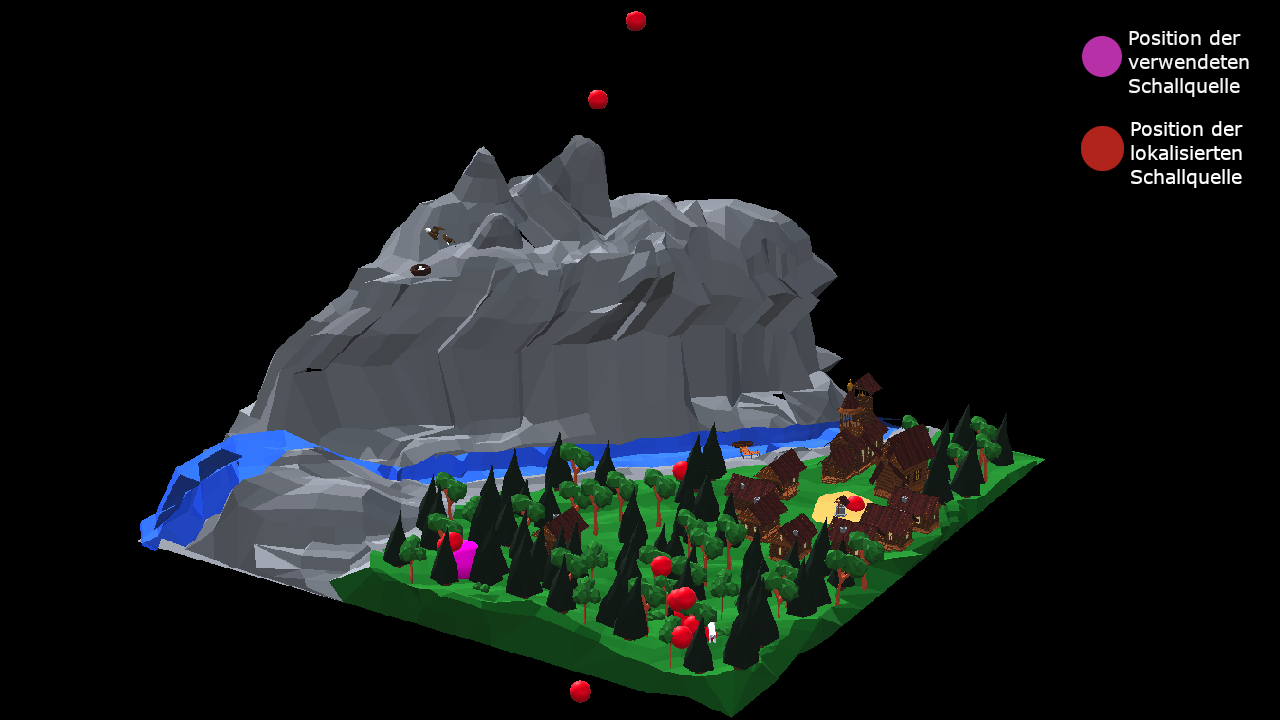
\includegraphics[width = 16cm, height = 9cm]{Szene_2_data.png}
\caption{Visualisierung der lokalisierten Schallquellen für Szene 2}
Der weiße Wolf wurde am häufigsten als Schallquelle lokalisiert, während nur wenige die wirkliche, virtuelle Schalle beim schwarzen Wolf entdeckt haben. 
\label{fig:Szene_2_data}
\end{figure} 

 
In Abbildung \ref{fig:Szene_2_data} lässt sich erkennen, dass ein Großteil der Probanden die virtuelle Schallquelle auf dem weißen Wolf lokalisiert hat und nur wenige an der Position des schwarzen Wolfes. Einige wenige haben die virtuelle Schallquelle außerhalb des Waldes, aber in der richtigen Höhe wahrgenommen und zwei Probanden haben die Hörereignisse wieder unmittelbar über dem Gebirge lokalisiert.  \\

Anscheinend konnte durch die räumliche Wiedergabe nicht darauf geschlossen werden, welcher der Wölfe die virtuelle Schallquelle darstellt. Da der weiße Wolf, etwas größer und von nicht so vielen Bäumen verdeckt worden ist, wurde das Hörereignis vermutlich eher in seiner Richtung lokalisiert. Es gilt also aufzupassen, dass beim Einsatz von räumlichem Audio nicht zu viele visuelle, potentielle Schallquellen im Raum sind, da es sonst zu Fehlinterpretationen bezüglich des Nutzers kommen könnte. 

\begin{figure}[H]
\centering
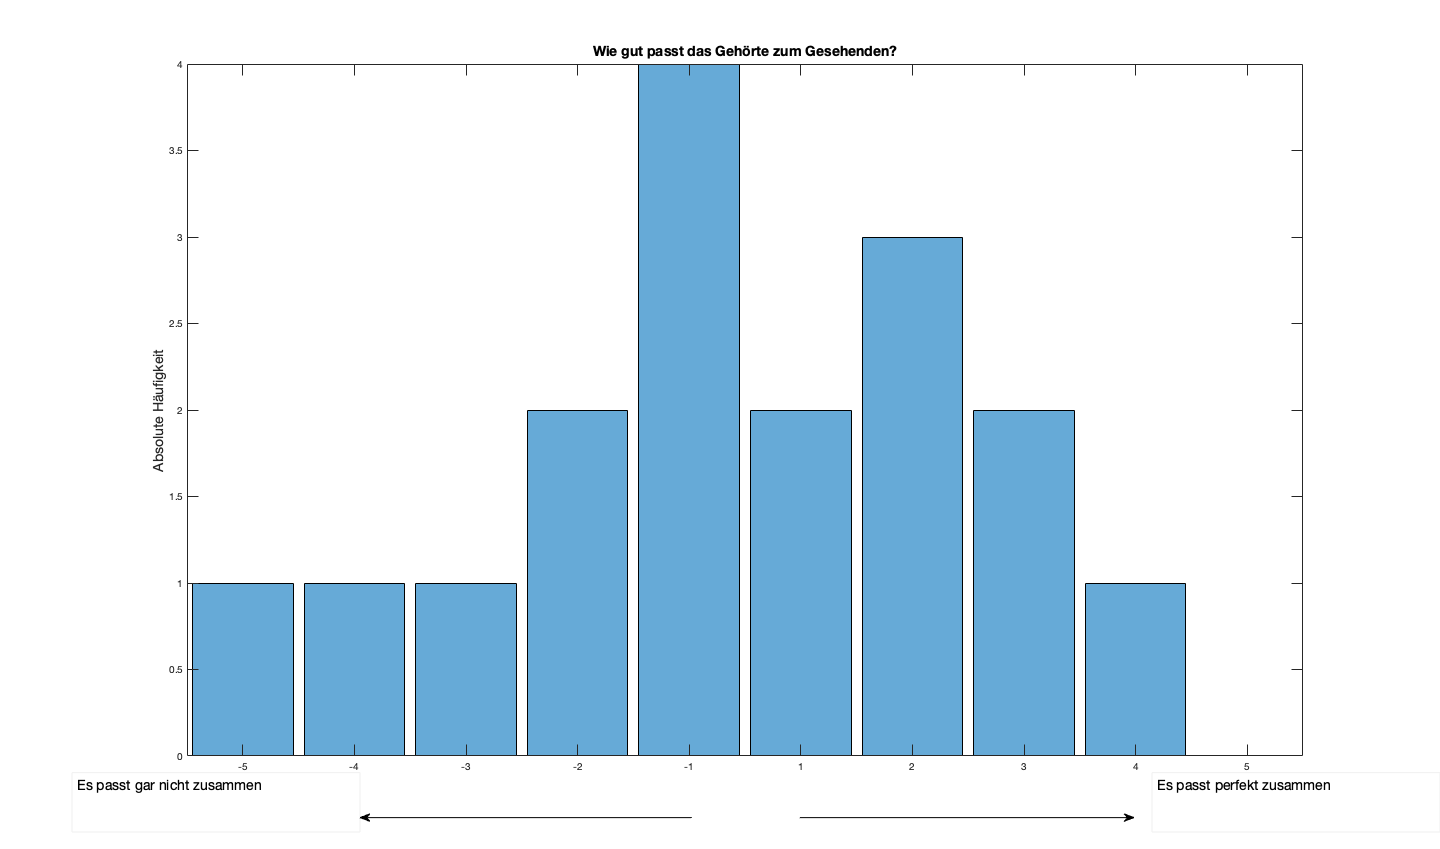
\includegraphics[width = 18cm, height = 10cm]{Szene_2_Frage_1.png}
\caption{Histogramm: Wie gut passen Visuelles und Auditives in Szene 2 zusammen ?}
Die wenigsten Probanden konnten einer der Aussage klar zustimmen. Für einige haben Visuelles und Auditives sehr gut zusammengepasst und für andere wiederum gar nicht. Generell wurde das Zusammenspiel positiver bewertet als bei der ersten Szene.
\label{fig:Szene_2_Frage1}
\end{figure} 

\vspace*{20pt}

Wie auch schon in der ersten Szene ist das Empfinden, ob das Visuelle und das Auditive zusammenpassen wieder sehr unterschiedlich, jedoch im Vergleich zur ersten Szene etwas positiver, siehe Abbildung \ref{fig:Szene_2_Frage1}. Während die meisten Probanden das Zusammenspiel wieder als mittelmäßig bewertet haben, so gibt es diesmal weniger die behaupten, dass das Gehörte und das Gesehene gar nicht zusammen passen würden. 

 \begin{figure}[H]
\centering
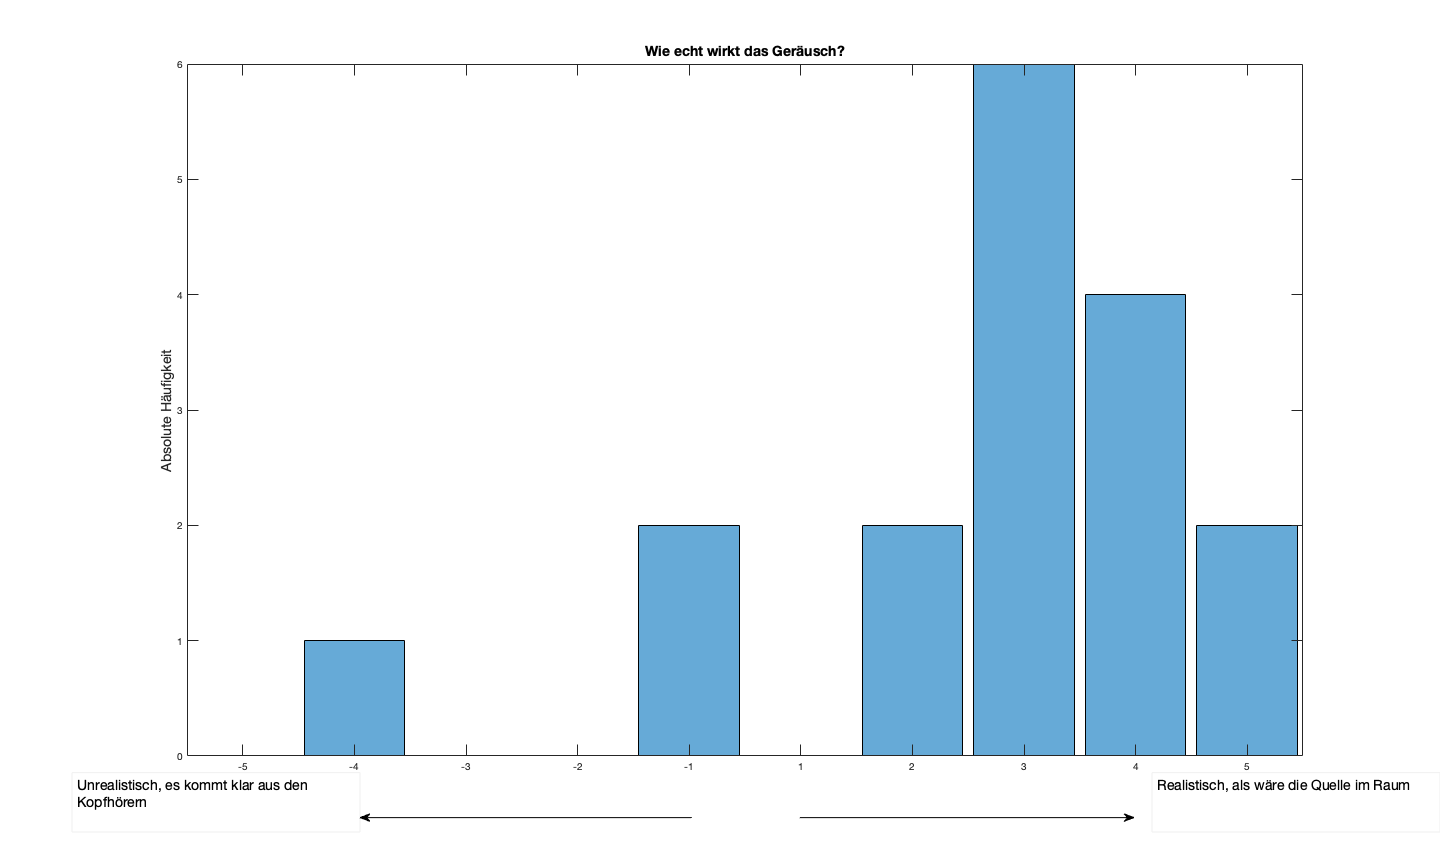
\includegraphics[width = 18cm, height = 10cm]{Szene_2_Frage_2.png}
\caption{Histogramm: Wie echt wirkt das Geräusch im Raum in Szene 2?}
Das Geräusch wurde von den meisten Probanden als realistische Schallquelle im Raum wahrgenommen.
\label{fig:Szene_2_Frage2}
\end{figure} 

\vspace*{20pt}


Anhand Abbildung \ref{fig:Szene_2_Frage2} lässt sich erkennen, dass das Geräusch als noch realistischer eingestuft worden ist als der Adlerschrei in Szene 1. Hierfür könnte es mehrere Gründe geben. Zum einen befindet sich die virtuelle Schallquelle in einer anderen Höhe als die der ersten Szene, so dass andere kopfbezogene Übertragungsfunktionen verwendet werden, die unter Umständen weniger gut zutreffend für die Probanden sind. Zum anderen könnte auch das Geräusch selbst ausschlaggebend sein.\\

Inhaltlich ist das Heulen eines Hundes bzw. Wolfes in einem Raum ein vertrauteres Geräusch als der Schrei eines Vogels, der vermutlich so niemals in einem Laborraum, auf der Höhe eines Tisches vorkommen wird. Die inhaltliche Einordnung des Geräusches könnte bewirken, dass das Heulen eines Hundes eher als plausibles Hörereignis im Raum wahrgenommen wird als der Schrei eines Adlers. 

\begin{figure}[H]
\centering
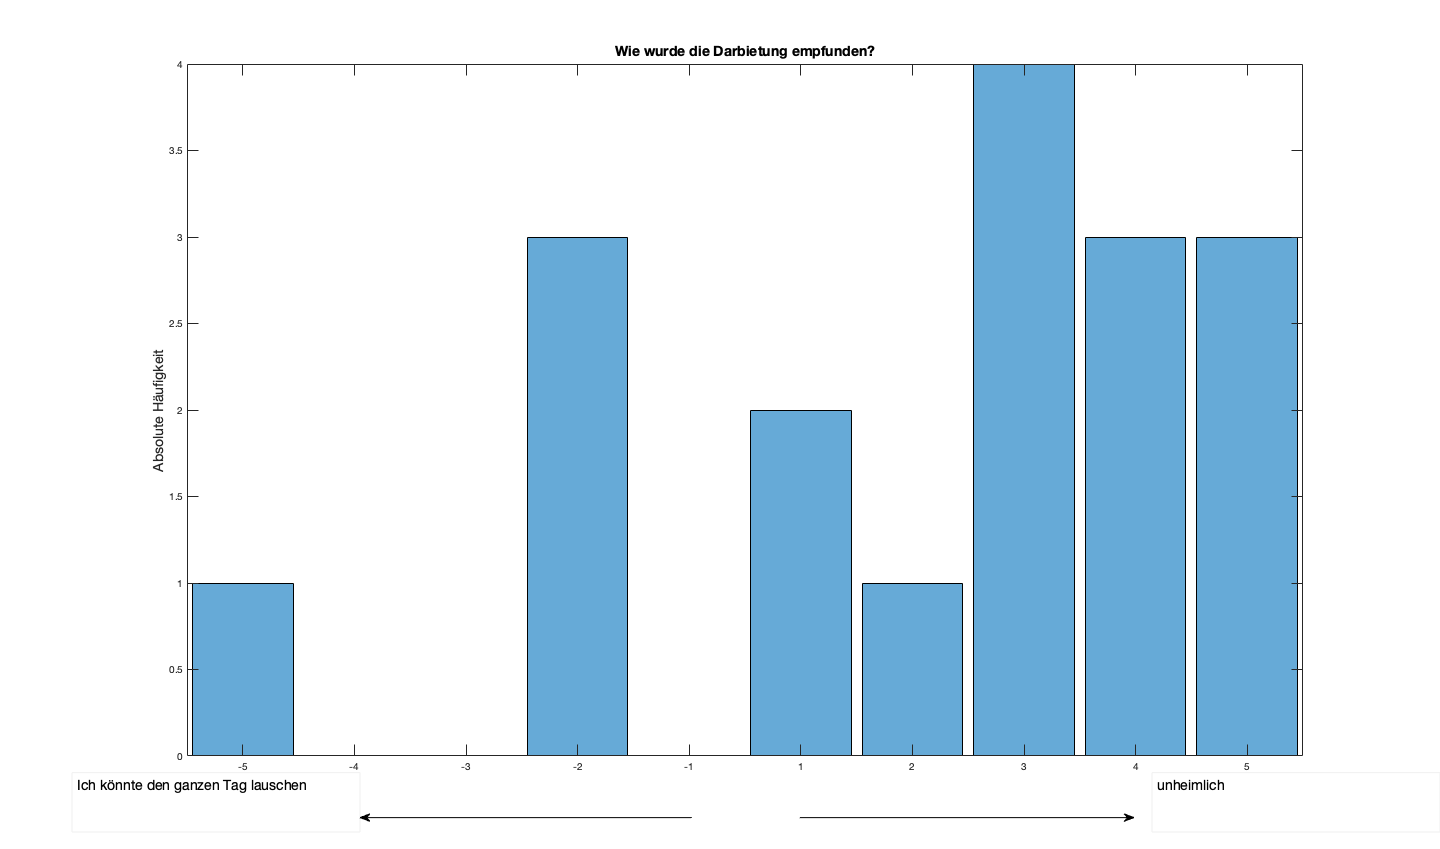
\includegraphics[width = 18cm, height = 10cm]{Szene_2_Frage_3.png}
\caption{Histogramm: Wie angenehm war die Darbietung von Szene 2?}
Für die meisten Probanden war die Darbietung äußerst unheimlich. Auf der anderen Seite gab es auch einige wenige Probanden, die die Darbietung als angenehm empfunden haben. 
\label{fig:Szene_2_Frage3}
\end{figure} 

\vspace*{20pt}

In Abbildung \ref{fig:Szene_2_Frage3} lässt sich erkennen, dass die Darbietung von Szene 2, genau wie die erste Szene, auf die meisten Probanden sehr unheimlich gewirkt hat, es jedoch auch mehr Ausnahmen gab als bei Szene 1. Ein Proband hat hierbei die Szene sogar mit der angenehmsten Bewertungsstufe versehen. Drei weitere Probanden haben die Szene ebenfalls als angenehm eingestuft. Das größtenteils evozierte Unwohlsein könnte, wie bei der vorherigen Szene, durch den zu hohen Realismus der Audio-Wiedergabe impliziert werden. \\ 

Ein anderer Grund für das Unwohlsein der Probanden bei der Szene könnte auch der inhaltliche Kontext des Geräusches sein. Dem Heulen eines Wolfes könnte mit Angst gegenübergetreten werden und dem Heulen eines Hundes mit Empathie. In beiden Fällen bedeutet dies, dass die Szene Unbehagen auslöst. An dieser Stelle ist hervorzuheben, dass der durch räumliches Audio implizierte Realismus der Geräusche natürlicherweise auch Gefahren, wie das Auslösen von Ängsten und Phobien beim Hörenden, birgt. \\

Wie schon bei der ersten Szene lässt sich anhand der Probandenergebnisse nicht wirklich beurteilen, wie gut eine Immersion der Probanden in die erweiterte Realität gelungen ist. Das empfundene Unbehagen der Probanden lässt auch in dieser Szene vermutlich keine Immersion zu. 

\newpage

 \subsection{Szene 3: Kirchenglocken}
Im Vergleich zu den ersten beiden Szenen wird in Szene 3 keine Form von räumlichen Audio verwendet. Stattdessen wird das Erklingen von Kirchenglocken mono über die Kopfhörer wiedergegeben.\\

\begin{figure}[H]
\centering
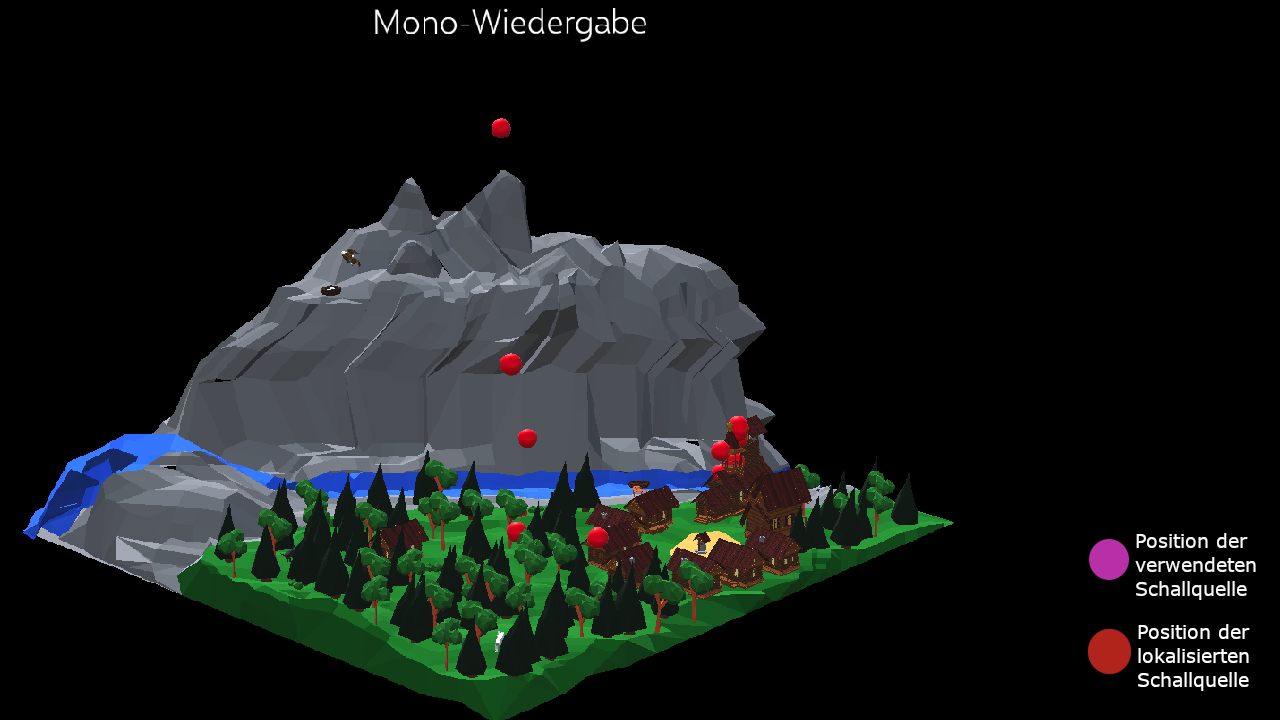
\includegraphics[width = 16cm, height = 9cm]{Szene_3_data.png}
\caption{Visualisierung der lokalisierten Schallquellen für Szene 3}
Trotz der Mono-Wiedergabe wurde die Schallquelle von fast allen Probanden im Kirchturm lokalisiert. Einige wenige haben sie jedoch in einer vertikalen in der Mitte der Welt lokalisiert. 

\label{fig:Szene_3_data}
\end{figure} 
\vspace*{30pt}
Wie anhand von Abbildung \ref{fig:Szene_3_data} zu sehen ist, lokalisieren die meisten Probanden das Hörereignis im vorderen Kirchturm. Daraus lässt sich schließen, dass auch ohne räumliches Audio die Schallquellen fast ausschließlich dort lokalisiert werden, wo es vom inhaltlichen Kontext her hin passt.\\

Auffällig sind hierbei die wenigen Ausreißer, die fast alle auf einer Vertikalen in der Mitte der virtuellen Welt liegen und dabei alle eine unterschiedliche Höhe haben. Dies liegt vermutlich daran, dass durch die Mono-Wiedergabe keine interauralen Laufzeitunterschiede zustande kommen und dies sonst nur der Fall ist wenn das zu lokalisierende Hörereignis in der Medianebene des Hörerenden liegt. Startet die Szene schaut der Proband zu aller erst gerade auf die Welt, so dass er denken könnte in dieser Ebene müsse die Schallquelle liegen.

\begin{figure}[H]
\centering
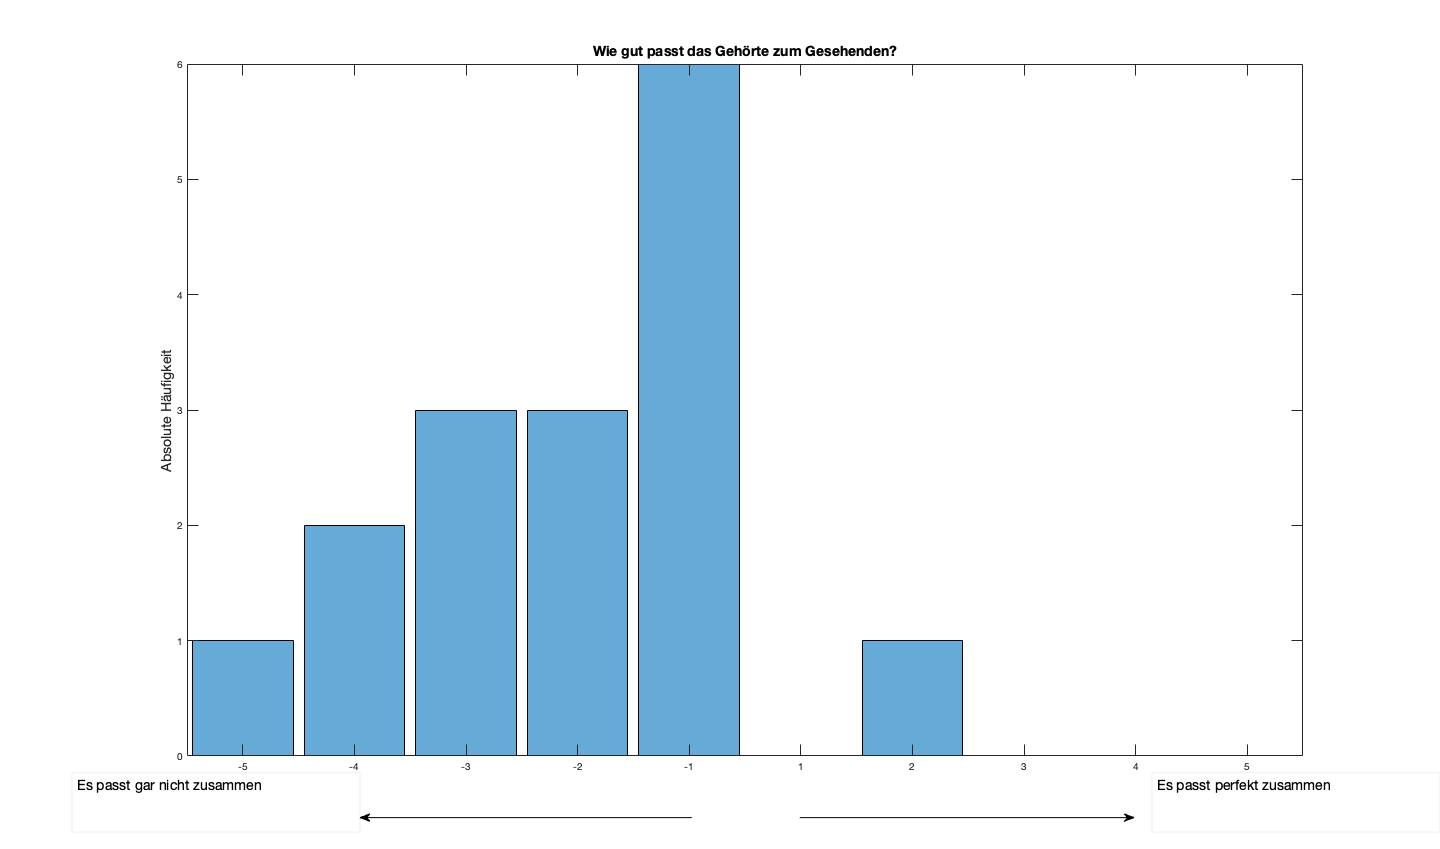
\includegraphics[width = 18cm, height = 10cm]{Szene_3_Frage_1.png}
\caption{Wie gut passen Visuelles und Auditives in Szene 3 zusammen?}
Von fast allen wurde das Zusammenspiel von visuellen und auditiven Inhalten als unplausibel eher unplausibel bewertet. Wobei auch sehr viele Probanden sich nicht wirklich festlegen konnten.
\label{fig:Szene_3_Frage1}
\end{figure} 
\vspace*{30pt}
Auch bei der Mono-Wiedergabe wurden das Visuelle und das Auditive als nicht zusammenpassend bewertet. Die Probanden sind sich bis auf einen einzigen einig, dass die Mono-Wiedergabe der Kirchenglocken gar nicht bis kaum zu den virtuellen Kirchenglocken passt.\\

Das Erklingen der Kirchenglocken hat keine räumliche Position und kann daher auch keiner visuellen Quelle zugeordnet werden. Der inhaltliche Kontext deutet jedoch darauf hin, dass die Quelle der Kirchturm in der Szene sein muss. Es ist daher die logische Konsequenz, dass bis auf einen Probanden sich alle dafür entschieden haben, dass die Darbietung unplausibel ist. 

\begin{figure}[H]
\centering
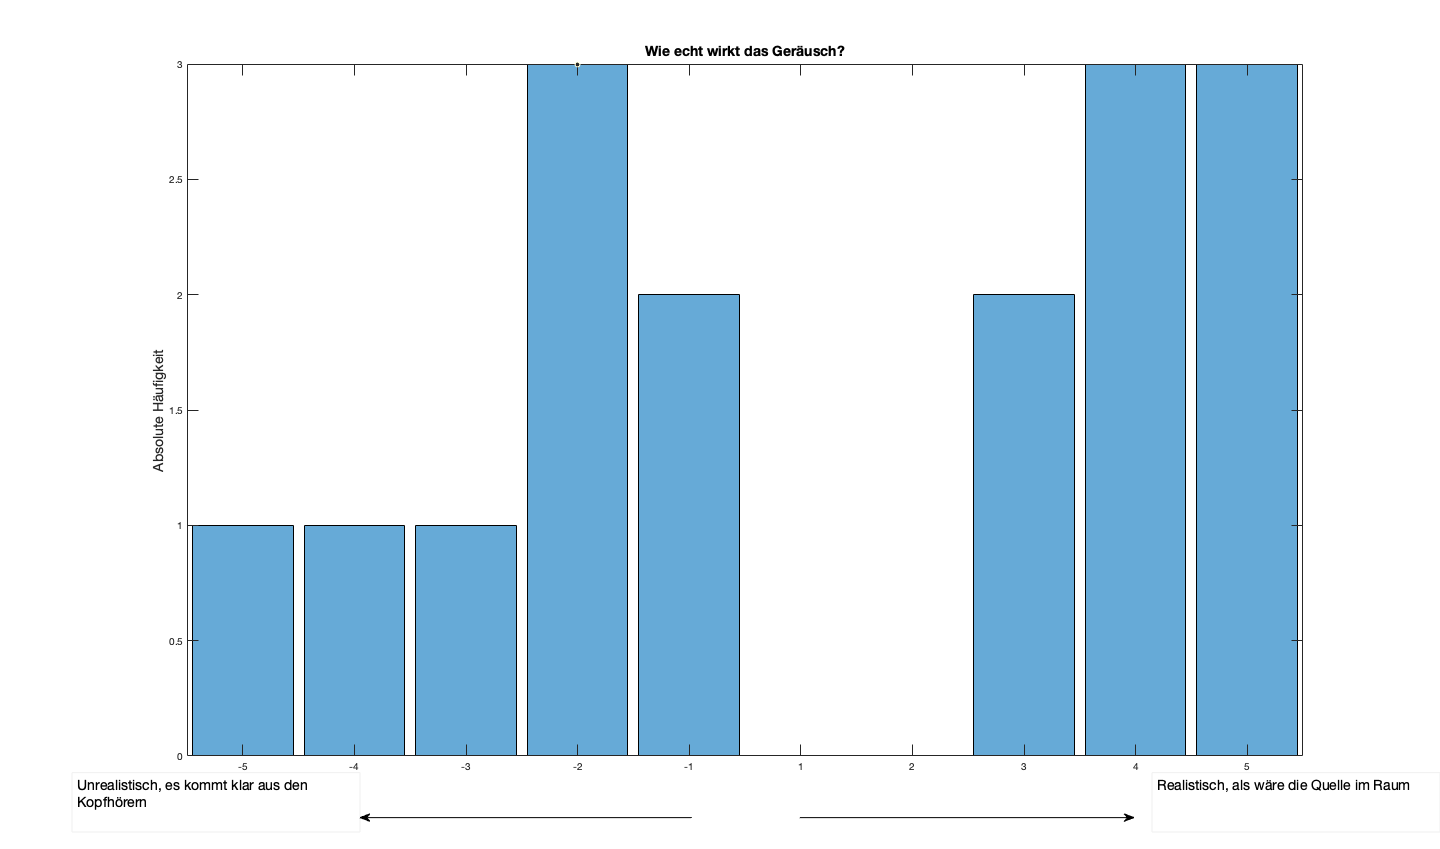
\includegraphics[width = 18cm, height = 10cm]{Szene_3_Frage_2.png}
\caption{Histogramm: Wie echt wirkt das Geräusch im Raum in Szene 3?}
Das Geräusch wurde sehr unterschiedlich, realistisch bewertet. Im Vergleich zu den anderen Szenen haben sehr viele das Geräusch als sehr unrealistisch bewertet. Viele Probanden haben das Geräusch, trotz der fehlenden räumlichen Wiedergabe, als realistisch empfunden.

\label{fig:Szene_3_Frage2}
\end{figure} 
\vspace*{30pt}

Überraschend ist, dass trotz der Mono-Wiedergabe ein Großteil der Probanden das Hörereignis als realistisches Geräusch im Raum wahrgenommen hat, wie es sich Abbildung \ref{fig:Szene_3_Frage2} erkennen lässt. Viele weitere Probanden haben das Geräusch als Teilweise unrealistisch wahrgenommen und nur wenige haben für sich entschieden, dass das Geräusch ganz offensichtlich aus den Kopfhörern kommt.\\

 Fraglich ist ob die Probanden, die die Szene als realistisch empfunden haben, den Unterschied zu den ersten Szenen nicht gehört haben, oder ob sie den wahrgenommenen Unterschied als irrelevant für die Bewertung des Realismus sehen. Mit der richtigen Ausführung könnte möglicherweise für viele Geräusche auf eine räumliche Audio-Wiedergabe verzichtet werden, ohne dass die Plausibilität der Szene verringert wird. 

 \begin{figure}[H]
\centering
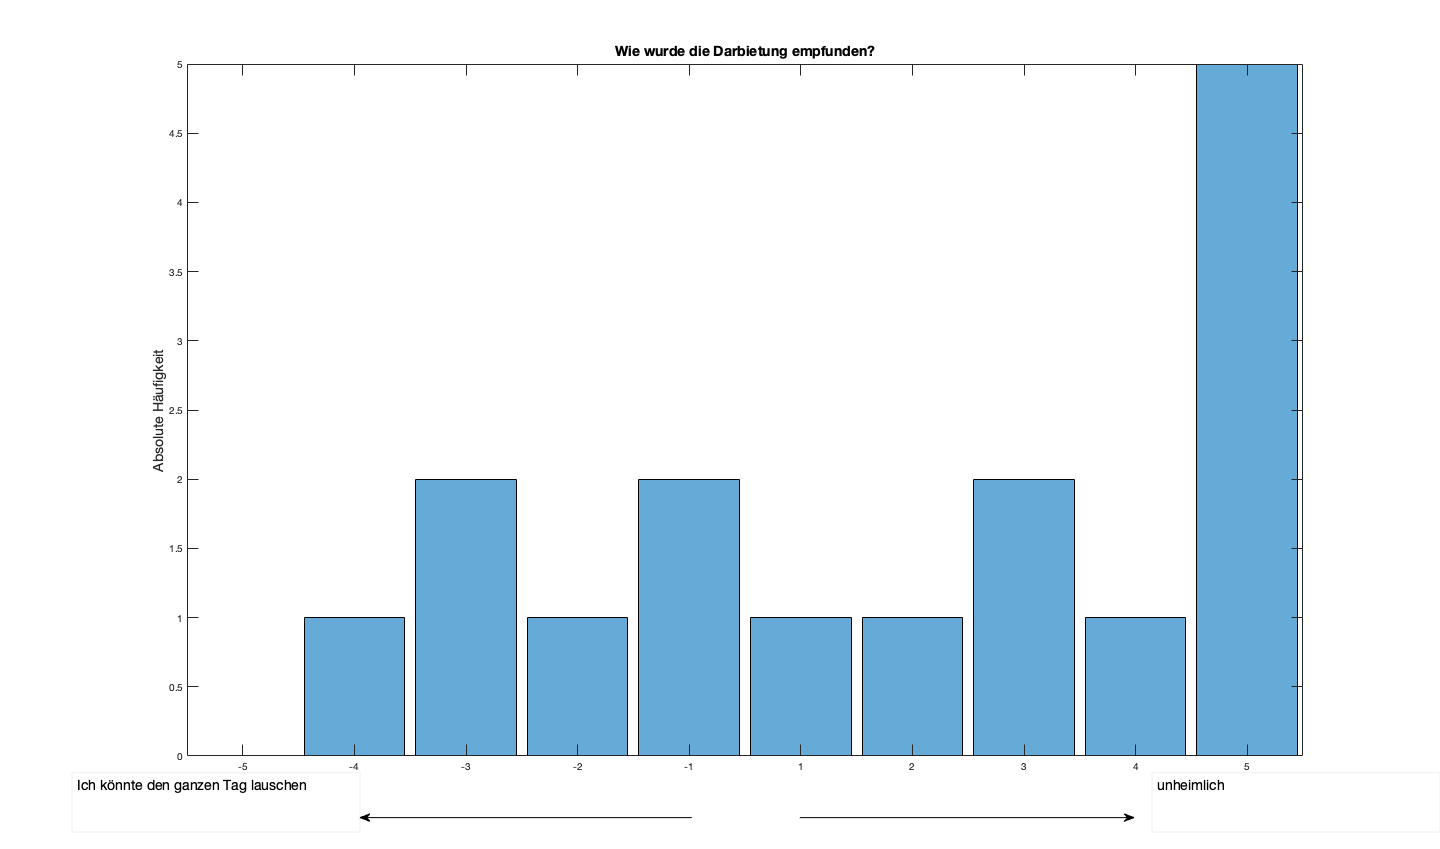
\includegraphics[width = 15cm, height = 8cm]{Szene_3_Frage_3.png}
\caption{Histogramm: Wie angenehm war die Darbietung von Szene 3?}
Die meisten Probanden haben die Darbietung erneut als unheimlich empfunden. Im Vergleich zu den anderen Szenen wurde es jedoch auch häufiger als angenehm bewertet.
\label{fig:Szene_3_Frage3}
\end{figure} 


In Abbildung \ref{fig:Szene_3_Frage3} lässt sich erkennen, dass wie bei den ersten beiden Szenen viele Probanden die Darbietung als unheimlich empfunden haben. Der Anteil an Probanden, die die Szene jedoch als angenehm empfunden haben ist beachtlich höher, als bei den ersten beiden Szenen. So empfinden sechs Probanden die Szene eher angenehm als unheimlich. \\

Ein Grund für das angenehmere Darbietungsempfinden könnte sein, dass das Erklingen von Glocken generell angenehmer ist, als das Heulen eines Wolfes oder der Schrei eines Adlers. Dies lässt sich unter anderem auch am bereits erwähnten harmonischen Klang des Geräusches  begründen.  \\

Natürlich könnte das im Vergleich zu den Szenen mit räumlichem Audio angenehmere Darbietungsempfinden auch das Resultat der fehlenden, räumlichen Anpassung der Audio-Signale sein, dessen extremer Realismus beim Hörenden Unbehagen bewirken könnte.

Mit fünf Probanden, die die Szene als komplett unheimlich bewertet haben und den Ergebnissen aus den vorherigen Szenen liegt es nah, dass die generelle Darbietung unabhängig vom Geräusch als unheimlich wahrgenommen werden könnte. Das Unwohlsein könnte dementsprechend auch einfach durch die ungewohnte Situation mit der HoloLens in einer Mixed-Reality-Umgebung evoziert werden. Diese Vermutung wird auch dadurch bekräftigt, dass während des Hörversuches sehr viele Probanden den unbequemen Halt und das zu kleine Sichtfeld der HoloLens  bemängelt haben. \\

Auch in der dritten Szene ist zu vermuten, dass die meisten Probanden, wie in dieser Szene zu erwarten war,  keine wirkliche Immersion empfinden konnten. Grund dafür ist, dass die visuellen und auditiven Reize erneut als nicht zusammenpassend empfunden worden sind, die Hörereignisse zudem eher als aus dem Kopfhörer kommend wahrgenommen worden sind und auch hier die Darbietung bei den meisten eher Unbehagen ausgelöst hat. 

 \subsection{Szene 4: Adlerschrei über dem Probanden}
In der vierten Szene werden wieder die Standart-Einstellungen für das räumliche Audio des Hörversuchs übernommen. Die virtuelle Schallquelle wurde hierbei über den Probanden platziert, so dass diese um den visualisierten Adler sehen zu können, nach oben schauen mussten. Bei dem Geräusch handelt es sich erneut um den Adlerschrei aus der ersten Szene. Im Vergleich zur ersten Szene sollte die Position des Geräusches nun besser an den inhaltlichen Kontext angepasst sein. \\

   \begin{figure}[H]
\centering
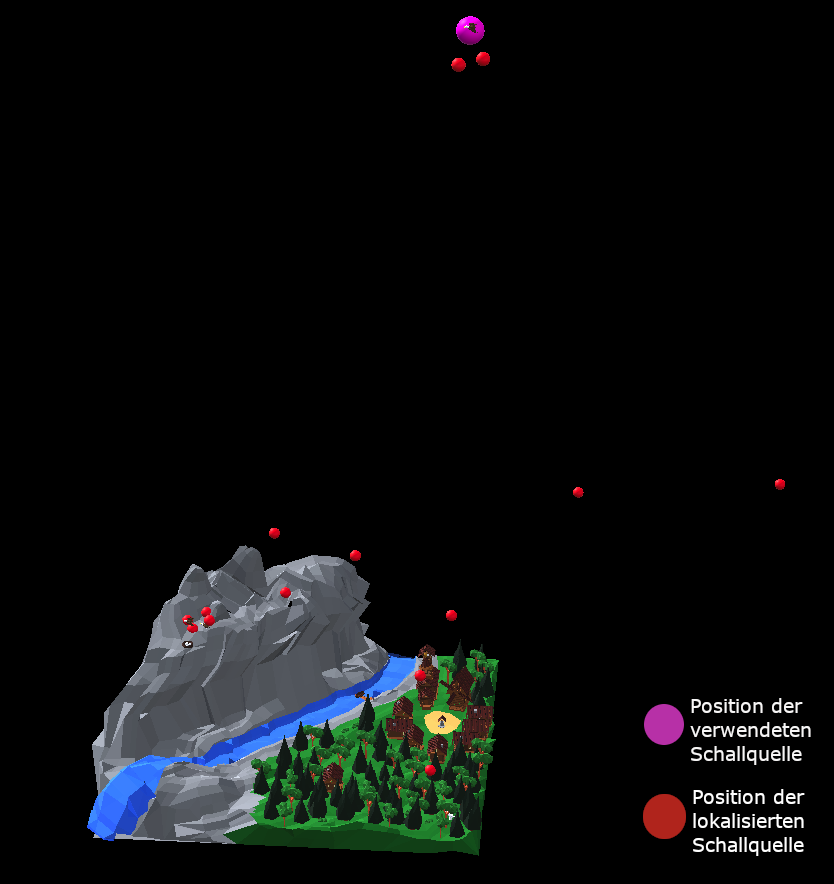
\includegraphics[width = 13cm, height = 14 cm]{Szene_4_data_2.png}
\caption{Visualisierung der lokalisierten Schallquellen für Szene 4}
Die Schallquelle wurde sehr gestreut lokalisiert. Nur zwei Probanden konnte den Adler über sich als virtuelle Schallquelle identifizieren. Einige haben den Adler über dem Berg als Schallquelle lokalisiert und andere haben wiederum die Schallquelle irgendwo im Raum erkannt. 
\label{fig:Szene_4_data}
\end{figure} 
\newpage

In Abbildung \ref{fig:Szene_4_data} ist zu erkennen, dass, wie bisher in keiner anderen Szene vorher, die virtuelle Schallquelle gestreut im Raum lokalisiert worden ist. Während zwei Probanden den Adler über sich ausmachen und als Schallquelle identifizieren konnten, haben vier andere Probanden erneut das Hörereignis beim Adler unmittelbar über dem Berg lokalisiert. \\

Bemerkenswert ist, dass die meisten Probanden erkennen konnten, dass das Hörereignis aus nicht mehr aus der Richtung der tiefer fliegenden Adler kommt und stattdessen die Schallquelle irgendwo im Raum lokalisiert haben. Dabei variieren zum ersten mal für die Szenen mit räumlichem Audio die Höhen der platzierten roten Kugeln. Die Probanden konnten also feststellen, dass die virtuelle Schallquelle über der Welt liegen muss, hatten aber Probleme ohne offensichtliche Visualisierung die richtige Position und die richtige Höhe zu ermitteln. Es ist anzunehmen, dass die meisten Probanden den Adler nicht mal sehen konnten, weil sie soweit oben keine Visualisierung mehr erwartet hätten. Der Einsatz von räumlichem Audio alleine reicht also nicht aus um den Fokus auf Objekte außerhalb des natürlichen Sichtfeldes zu legen. 
\vspace*{30pt}
   \begin{figure}[H]
\centering
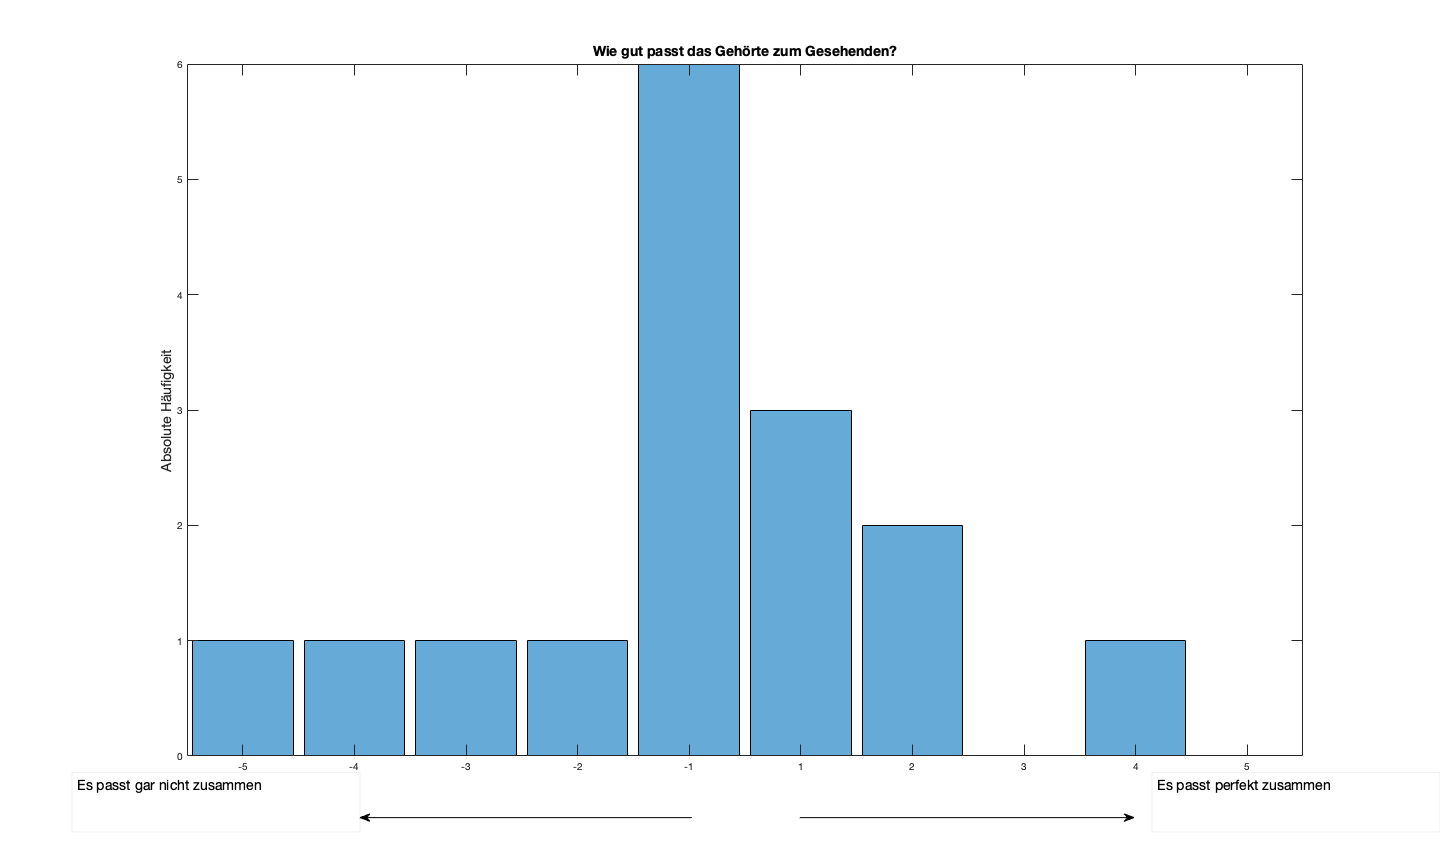
\includegraphics[width = 18cm, height = 10cm]{Szene_4_Frage_1.png}
\caption{Histogramm: Wie gut passen Visuelles und Auditives in Szene 4 zusammen ?}
Fast alle Probanden konnten in dieser Szene keiner der gestellten Aussagen zustimmen. Der Anteil der Probanden für die das Gesehene und das Gehörte zusammenpassen ist genauso groß, wie der Anteil für die es gar nicht zusammenpasst.
\label{fig:Szene_4_Frage1}
\end{figure} 
\newpage
In Abbildung \ref{fig:Szene_4_Frage1} lässt sich erkennen, dass im Vergleich zur ersten Szene, mit dem selben Geräusch, das Empfinden, ob Visuelles und Auditives zusammenpassen, tatsächlich etwas positiver ausfällt. Während in der ersten Szene noch für sechs Probanden das Gehörte und das Gesehene sehr wenig bis gar nicht zusammengepasst haben, so gibt es bei der vierten Szene  nur noch 3 Probanden die das Zusammenspiel so negativ bewertet haben. Der Zahl der Probanden, die bei der Frage keiner der Antworten wirklich zustimmen konnten ist hierbei stark gestiegen, während der Anteil der Probanden für die die Reize zusammen gepasst haben gleich geblieben ist. \\ 

Es gilt bei der Beobachtung der Ergebnisse dieser Umfrage zu beachten, dass vermutlich die wenigsten den Adler über sich wirklich gesehen haben. Das leicht verbesserte Empfinden für das Zusammenspiel des Auditiven mit dem Visuellen könnte daher unterschiedliche Gründe haben. Einer der Gründe könnte sein, dass dadurch das der Adlerschrei nun aus der Luft kommt die allgemeine Plausibilität der Szene gestiegen ist, da der inhaltliche Kontext besser zum Gesehenen passt. Ein weiterer Grund könnte sein, dass der Proband sich generell an das Tragen der HoloLens und den Anblick der Welt gewöhnt hat und daher das Visuelle anders wahrnimmt. \\ 

Dass sich viele gar nicht entscheiden konnten ob Visuelles und Auditives zusammenpassen, hängt vermutlich damit zusammen, dass sie den Adler nicht sehen konnten und sich damit nicht in der Lage gefühlt haben das Zusammenspiel überhaupt bewerten zu können. 

 \begin{figure}[H]
\centering
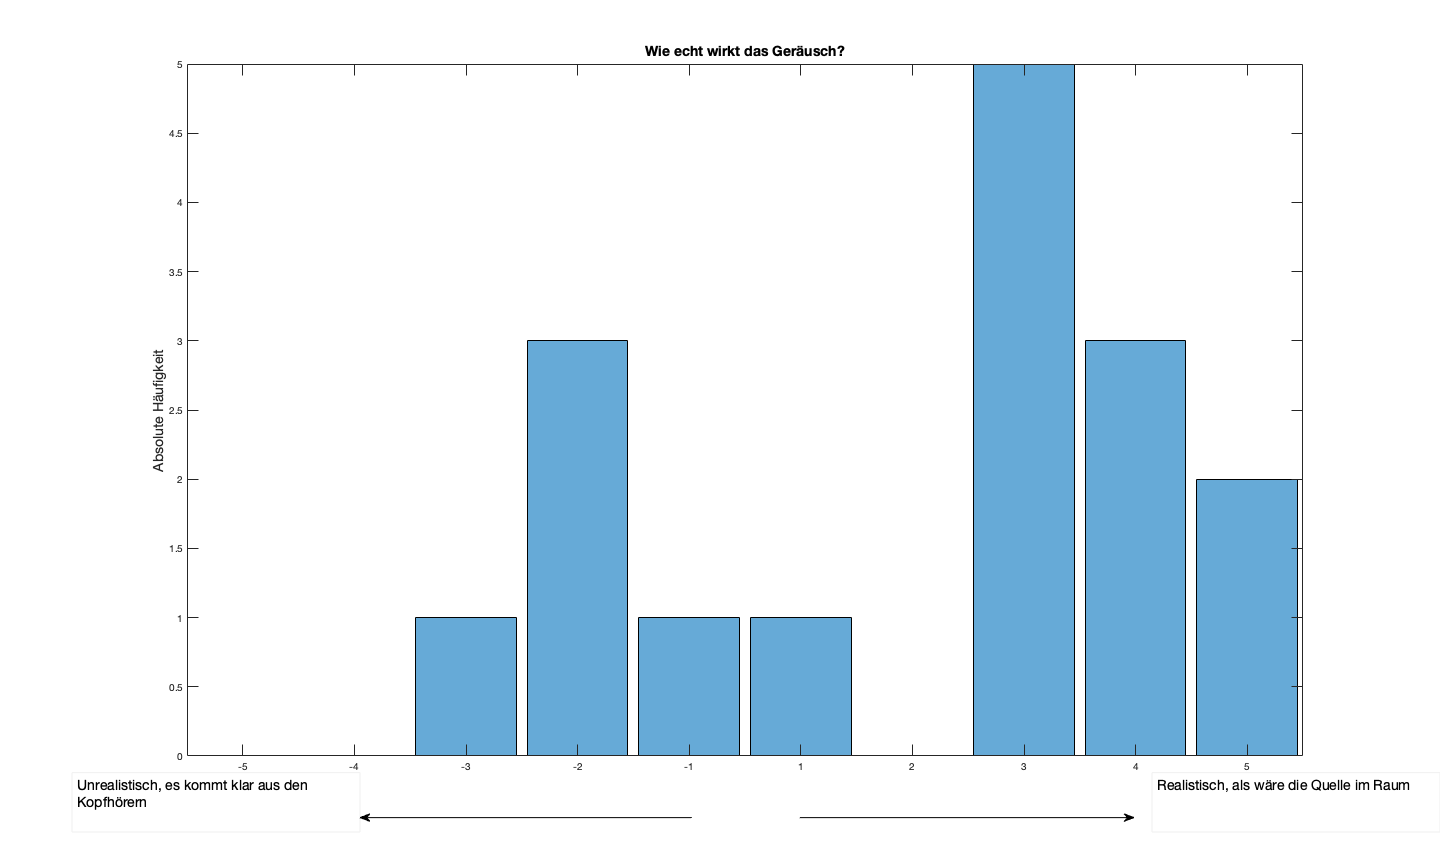
\includegraphics[width = 18cm, height = 10cm]{Szene_4_Frage_2.png}
\caption{Histogramm: Wie echt wirkt das Geräusch im Raum in Szene 4?}
Für den Großteil der Probanden war die räumliche Wiedergabe äußerst plausibel. Der Anteil der Probanden, die es als unrealistisches Geräusch wahrgenommen haben, ist im Vergleich zu anderen Szenen etwas höher.  
\label{fig:Szene_4_Frage2}
\end{figure} 

\newpage

Anhand Abbildung \ref{fig:Szene_4_Frage2} ist zu sehen, dass zehn Probanden das Geräusch als realistische Quelle im Raum beurteilen würden. Damit sind es sogar noch mehr als bei der ersten Szene, die das Geräusch als realistisch beurteilen. Angestiegen ist jedoch auch der Anteil, der Probanden, die das Geräusch als unrealistisch bewerten. \\

Die Ergebnisse könnten damit zu begründen sein, dass die meisten Probanden erkannt haben, dass das Hörereignis nicht mehr unmittelbar in der virtuellen Welt stattgefunden hat und es deshalb als plausibler eingestuft worden ist. Gleichzeitig konnten einige, wie es in Abbildung \ref{fig:Szene_4_data} gezeigt wird, nicht erkennen, dass das Geräusch nicht mehr dort ist wo es sich noch in der ersten Szene befand. Geht man davon aus, dass das Geräusch wirklich noch auf den Adlern über dem Berg liegt, dann klingt das Audio-Signal, das an den Adler über dem Probanden angepasst worden ist, natürlich unplausibel und daher unrealistisch. 

\begin{figure}[H]
\centering
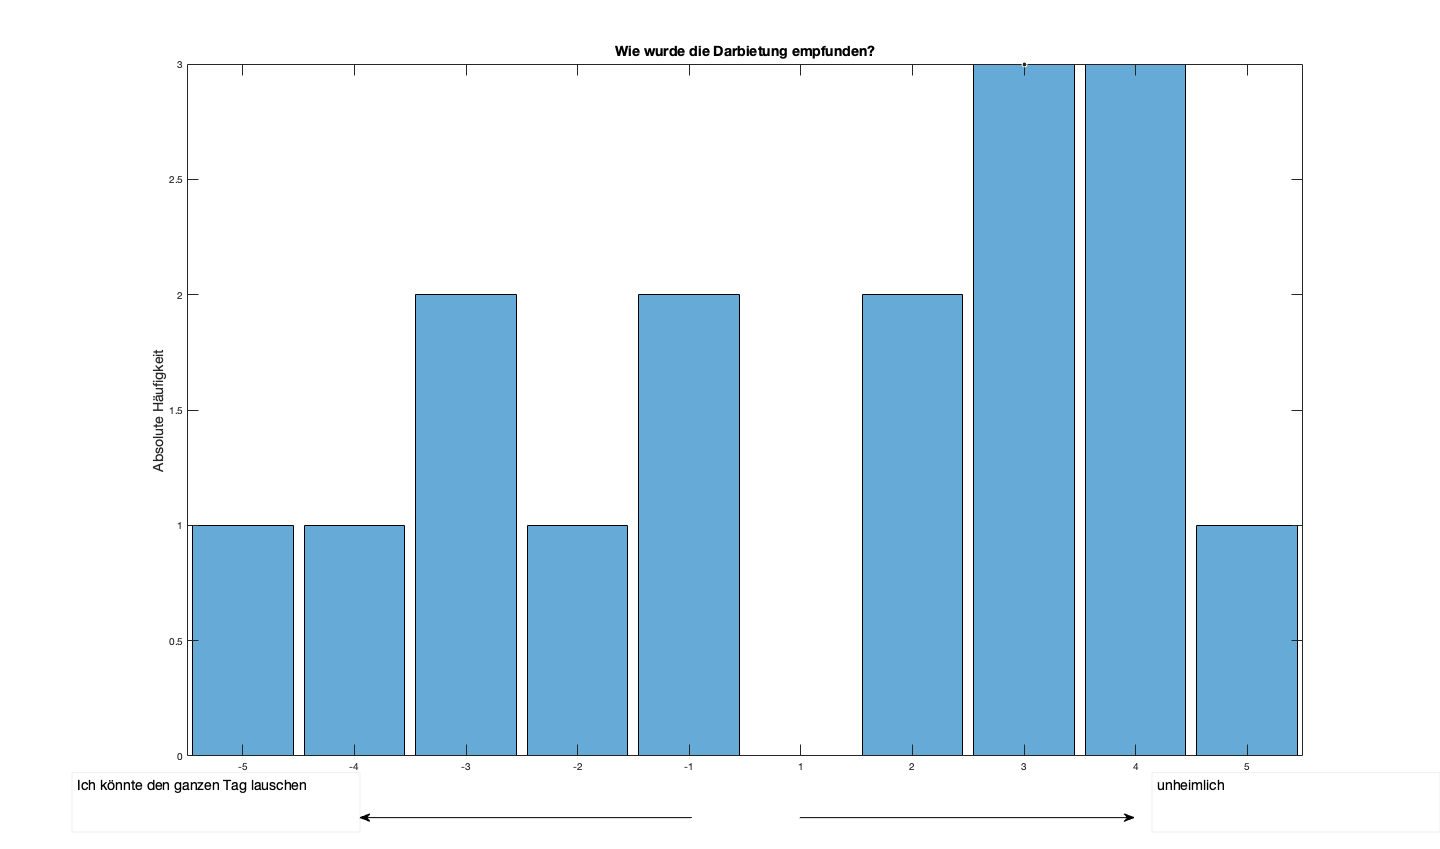
\includegraphics[width = 18cm, height = 10cm]{Szene_4_Frage_3.png}
\caption{Histogramm: Wie angenehm war die Darbietung von Szene 4?}
Im Vergleich zu anderen Szenen haben sehr viele die Darbietung als angenehm bewertet, während diese bei einem Großteil immer noch Unbehagen auslöst.  
\label{fig:Szene_4_Frage3}
\end{figure} 
\vspace*{30pt}
Die Darbietung von Szene 4 wurde, wie es in Abbildung \ref{fig:Szene_4_Frage3} gezeigt wird,  von vielen Probanden als deutlich angenehmer empfunden als die Darbietung der ersten beiden Szenen. Während bei der ersten Szene noch ca. 90 \% der Probanden die Darbietung eher als unheimlich empfunden haben, so haben in der vierten Szenen schon mehr als 40 \% die Darbietung als eher angenehm bewertet. Trotz dessen evoziert die Darbietung bei den meisten immer noch ein eher unangenehmes Gefühl.\\ 

Das zunehmend positivere Darbietungsempfinden der Szene könnte damit zusammenhängen, dass wie bereits erwähnt das Geräusch einfach, dadurch dass es von oben kommt, inhaltlich plausibler ist. Andererseits könnte die Darbietung auch durch die Gewöhnung der Probanden an die HoloLens immer angenehmer werden. \\ 

Theoretisch könnte aber auch die Tatsache, dass das Hörereignis nicht mehr in der unmittelbaren Umgebung des Hörenden liegt dafür verantwortlich sein, dass die Darbietung nicht mehr so unheimlich bewertet wird, wie bei den anderen Szenen. Möglicherweise tritt der vermute \glqq Uncanny-Valley\grqq{}-Effekt nur dann für realistisches, räumliches Audio auf, wenn sich das Geräusch direkt vor dem Betrachter, bzw. im Sichtfeld, befindet. Da die meisten erkannt haben, dass das Hörereignis nicht direkt in der virtuellen Welt stattgefunden hat, könnte es sein, dass sie sich von diesem Geräusch auch nicht eingeschüchtert oder bedroht gefühlt haben.
 
 \subsection{Szene 5: Flussrauschen}
Die letzte Szene des Versuchs enthält im Vergleich zu den anderen Szenen zwei virtuelle Schallquellen. Als Geräusch wird das Rauschen eines Flusses über beide Schallquellen gleichermaßen wiedergegeben. Der Proband hat auch hier nur eine Kugel zu platzieren, da erwartet wird, dass sich eine Phantomschallquelle bilden müsste. Auch hier werden die für den Versuch gewählten Standart-Einstellungen verwendet. Die eine Schallquelle befindet sich hierbei an der Quelle des Flusses und die andere den Fluss abwärts im Boot. \\ 

\begin{figure}[H]
\centering
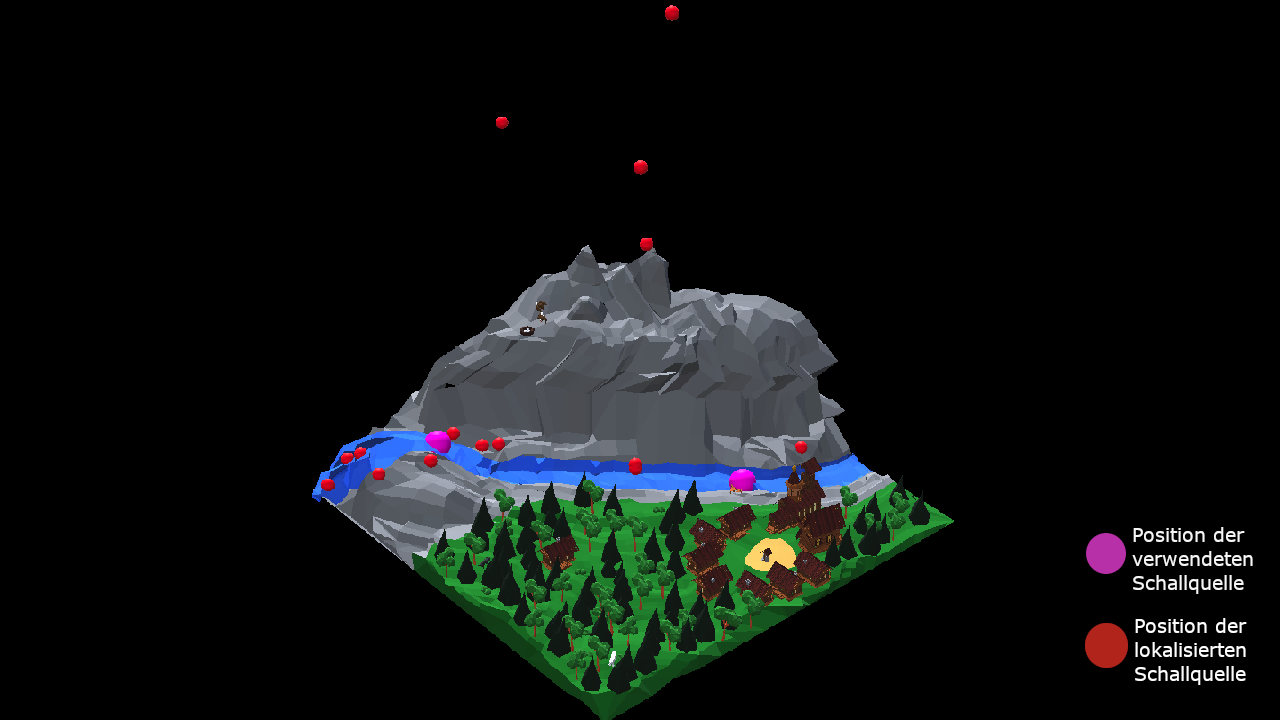
\includegraphics[width = 16cm, height = 9cm]{Szene_5_data.png}
\caption{Visualisierung der lokalisierten Schallquellen für Szene 5}
Die Schallquelle wurden von fast allen Probanden an der Quelle des Fluss lokalisiert. Einige haben sie jedoch auch über dem Gebirge und einige in der Mitte des Flusses lokalisiert. 
\label{fig:Szene_5_data}
\end{figure} 
\vspace*{30pt}
Abbildung \ref{fig:Szene_5_data} zeigt, dass das Hörereignis erneut sehr weit gestreut lokalisiert worden ist. Die meisten Probanden haben dabei das Hörereignis an der Quelle des Flusses wahrgenommen. Hierbei ist zu erwähnen, dass die Probanden fast ausschließlich beim Lokalisieren stehengeblieben sind und daher diese virtuelle Schallquelle näher an den Probanden positioniert gewesen ist, als die zweite Schallquelle im Boot. Nach dem Prinzip der ersten Wellenfront ergibt es also Sinn, dass die Probanden das Hörereignis fast ausschließlich bei der näheren virtuellen Schallquelle wahrgenommen haben, da der Schall dieser Quelle zu erst beim Probanden angekommen ist. Des Weiteren ist davon auszugehen, dass der inhaltliche Kontext eine Rolle bei der Platzierung der roten Kugel gespielt haben könnte, da das Flussrauschen in der Natur vor allem in der wilderen Gebirgslandschaft erwartet werden würde.\\

Zwei Probanden haben die rote Kugel genau in der Mitte zwischen den beiden virtuellen Schallquellen platziert. Dies ergibt vor allem dann Sinn, wenn die Probanden sich so bewegt hätten, dass die virtuellen Schallquellen beide gleich weit vom Probanden entfernt gewesen sind. Ist dies der Fall, dann sollte sich das Hörereignis aufgrund der fehlenden interauralen Laufzeitunterschiede genau in der Mitte der beiden virtuellen Schallquellen bilden. Drei weitere Probanden haben das Hörereignis auf einer Vertikalen zur Welt, mittig zwischen den virtuelle Schallquellen, lokalisiert. Bei diesen hat sich das Hörereignis also ebenfalls mittig zwischen den virtuellen Schallquellen gebildet, jedoch haben diese Probanden die Höhe des Hörereignisses anders wahrgenommen.\\ 

An diesem Punkt sollte erwähnt werden, dass bei einer ausgereifteren Version des Hörversuchs neben der Position der roten Kugel auch die Position des Probanden, während der Platzierung gespeichert werden sollte. Auf diese Weise könnten bessere Aussagen darüber getroffen werden, wieso der Proband das Hörereignis so lokalisiert hat, wie er es während des Hörversuchs getan hat. 

\begin{figure}[H]
\centering
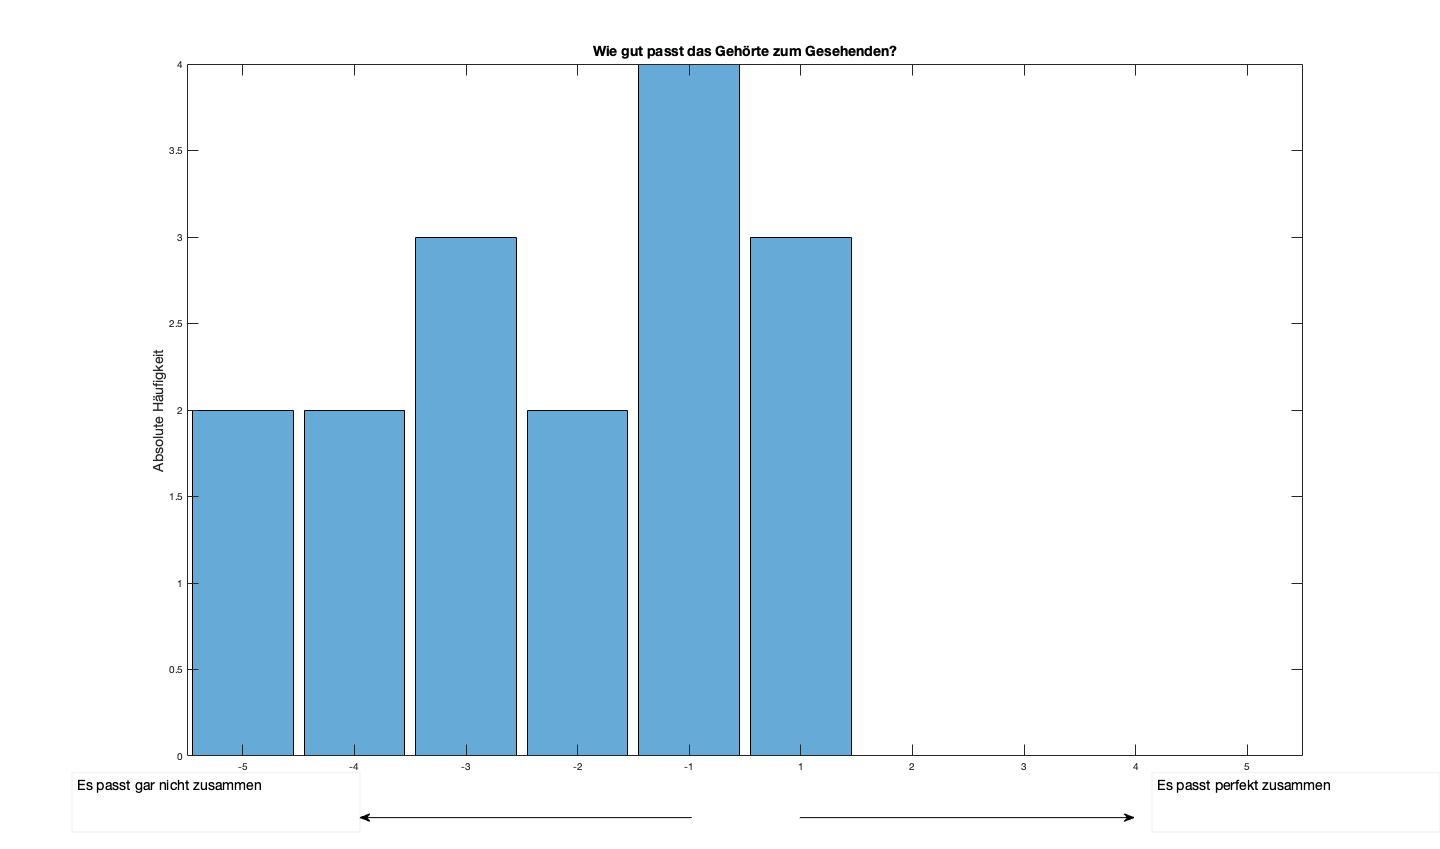
\includegraphics[width = 18cm, height = 10cm]{Szene_5_Frage_1.png}
\caption{Histogramm: Wie gut passen Visuelles und Auditives in Szene 5 zusammen?}
Die meisten Probanden gaben an, dass für sie das Visuelle nicht zum Auditiven gepasst hat. Während ein Großteil der Probanden wiederum keiner der beiden Aussagen wirklich zustimmen konnte, hat niemand das Zusammenspiel als wirklich plausibel bewertet. 
\label{fig:Szene_5_Frage1}
\end{figure} 
\vspace*{30pt}

Anhand Abbildung \ref{fig:Szene_5_Frage1} lässt sich feststellen, dass die Probanden sich bei der letzten Szene ziemlich einig sind, dass das Gesehene und das Gehörte nicht sehr gut zusammen passen. Während sieben Probanden keiner der Aussagen komplett zugestimmt haben, so hat der Rest der Probanden das Visuelle und das Auditive als wenig bis gar nicht zusammenpassend bewertet. \\

Das Fließen eines Flusses ist ein sehr dynamischer Vorgang, der wie das Flussrauschen vermutlich mit sehr viel Bewegung assoziiert wird. Es ist daher davon auszugehen, dass das statische blaue Wasser in der virtuellen Welt ohne Animation nicht als plausibler visueller Reiz wahrgenommen werden kann. Unter anderem gilt dies auch, weil sich das Wasser in der virtuellen Welt nicht nach den Gesetzen der Physik verhält und einfach in der Luft schwebt ohne abzufließen. \\

   \begin{figure}[H]
\centering
\includegraphics[width = 18cm, height = 10cm]{Szene_5_Frage_2.png}
\caption{Histogramm: Wie echt wirkt das Geräusch im Raum in Szene 5?}
Bis auf drei Probanden haben alle die räumliche Wiedergabe als äußerst plausibel bewertet. 
\label{fig:Szene_5_Frage2}
\end{figure} 
\vspace*{30pt}

Wie sich in Abbildung \ref{fig:Szene_5_Frage2} erkennen lässt, sind auch bei der Frage, wie echt denn das Geräusch in der letzten Szene wirke, die Probanden fast ausschließlich der Meinung, dass sich das Geräusch sehr realistisch angehört hat.  Bis auf drei Probanden, die die räumliche Wiedergabe als eher unplausibel bewertet haben, sind die restlichen Probanden der Meinung, dass sich das Geräusch wirklich so angehört hat, als ob die Quelle im Raum wäre.\\ 

Von allen Szenen des Hörversuches wurde das Geräusch dieser Szene als realistischstes Hörereignis bewertet. Der Einsatz mehrerer Schallquellen liefert damit also auch mit räumlichem Audio recht plausible Hörereignisse und kann unter anderem dafür genutzt werden größere, virtuelle Objekte auditiv zu unterstützen. \\ 


   \begin{figure}[H]
\centering
\includegraphics[width = 18cm, height = 10cm]{Szene_5_Frage_3.png}
\caption{Histogramm: Wie angenehm war die Darbietung von Szene 5?}
Die Darbietung wurde wieder als sehr unheimlich bewertet. Für nur drei Probanden war die Darbietung angenehm.
\label{fig:Szene_5_Frage3}
\end{figure} 
\vspace*{10pt}

Abbildung \ref{fig:Szene_5_Frage3} zeigt, dass auch beim letzten Versuch die Darbietung wieder als überwiegenden unheimlich bewertet worden ist. Bis auf drei Ausnahmen haben wieder alle Probanden die Darbietung als unheimlich empfunden. Bei keiner Szene vorher wurde hierbei häufiger die maximale Ausprägung des unheimlichen Darbietungsempfindens ausgewählt, als bei der letzten Szene.\\ 

Auch bei der letzten Szene korrelieren damit die Ergebnisse zum empfunden Realismus des Geräusches mit dem evozierten unheimlichen Darbietungsempfinden. Die These, dass eine realistische Umsetzung von räumlichem Audio Unbehagen auslösen könnte wurde somit durch keine der Darbietungen entschärft und hat weiterhin Bestand. 
\section{Versuchskritik}
Der Hörversuch ist in großen Teilen gelungen. Er konnte einen Einblick liefern, wie gut die Lokalisation von virtuellen Schallquellen mit räumlichem Audio möglich ist und welche Herausforderungen dabei auf Entwickler zukommen. Dennoch muss erwähnt werden, dass der Versuch in vielerlei Hinsicht besser hätte durchgeführt werden können. \\

Anfangend mit der Versuchsumgebung lässt sich sagen, dass der Versuchsraum, in Form des DSP-Labors E113 der Hochschule Emden/Leer, kein optimaler Ort für einen Hörversuch ist. Es befindet sich in diesem Raum sehr viel Technik und andere Gegenstände, die nicht für den Hörversuch benötigt worden sind. Die Umgebung könnte die Probanden also mehr oder weniger stark, während des Versuchs abgelenkt und damit die Ergebnisse beeinflusst haben. Außerdem sorgen die unnötigen Gegenstände und Möbel im Raum dafür, dass das in die Applikation integrierte Raummodell zur Auralisation nicht komplett vollständig ist. Die Anpassung der Audio-Signale an den Raum konnte somit nicht vollends detailliert durchgeführt werden. Dennoch wurden die Geräusche größtenteils als realistisch bewertet, weshalb dieser Punkt zu vernachlässigen ist. \\

Ein zusätzliches Problem der Umgebung war der Umgebungslärm. Zum einen war direkt vor dem Fenster eine Baustelle dessen Lärm, zwar durch die Fenster gedämpft wurde, jedoch trotzdem hörbar war und damit Einfluss auf die Probanden gehabt haben könnte. Des Weiteren haben diejenigen, die auf die Durchführung des Hörversuchs anderer warten mussten, sich sehr leise in der Nähe der Versuchsperson unterhalten. Auch dies könnte eine Immersion des Probanden in die erweiterte Realität verhindert haben. Dennoch muss hierbei erwähnt werden, dass die Störschallunterdrückung des Menschen solche Nebengeräusche bewusst filtern kann. \\

Neben der verbesserungswürdigen Versuchsumgebung lässt sich auch die Versuchsdurchführung kritisch hinterfragen. Zum einen sollte der Versuch für wirklich aussagekräftige Ergebnisse mit deutlich mehr Probanden durchgeführt werden, was leider im Rahmen dieser Bachelorarbeit nicht möglich gewesen ist. \\ 

Des Weiteren hätten bei der Durchführung mehr Informationen zu den Probanden aufgenommen werden müssen, die alle Einfluss auf die Ergebnisse gehabt haben könnten. Unter anderem die Größe, das Alter und ob die Probanden eine bestimmte Einschränkung, wie eine Seh- oder Hörschwäche haben, können großen Einfluss auf die Lokalisationsfähigkeit haben. \\

Auch das Verhalten der Probanden hätte auf irgendeine Art und Weise dokumentiert werden müssen. Ob sich der Proband viel oder wenig Zeit bei der Lokalisation der virtuellen Schallquelle gelassen hat und ob sich dieser währenddessen viel oder wenig bewegt hat, sind beides Indizien für die Aussagekraft der Ergebnisse. Für die richtige Durchführung dieses Hörversuches hätte es dementsprechend ein deutlich größeres Team und mehr Entwicklungszeit benötigt. \\

Es könnte außerdem darüber diskutiert werden, inwiefern die gestellten Fragen genau so zu deuten sind, wie es in der Bachelorarbeit letztlich getan worden ist. Ein Problem der Arbeit war es die wichtigsten Kriterien für VR und AR, wie beispielsweise Plausibilität und Immersion bewerten zu lassen ohne dabei zu technische Fragen zu stellen. Aus diesem Grund wurde versucht anhand abstrakter Fragen mit vorgegebenen, gewichtbaren Antwortmöglichkeiten einen ungefähren Eindruck vom Darbietungsempfinden des Probanden zu erhalten. \\

Der letzte Kritikpunkt lag in der Bedienbarkeit der Applikation. Viele der Probanden hatten Probleme damit die HoloLens an sich zu bedienen und empfanden dies auch als äußerst unangenehm. Dementsprechend waren die in der Applikation benötigten Bedienelemente für manche Probanden, die bisher wenig bis gar nicht mit AR und VR in Kontakt getreten sind, sehr schwierig zu verwenden. Bei der Analyse der Ergebnisse musste dementsprechend beachtet werden, dass einige Probanden die Position der lokalisierten Hörereignisse nur ungefähr angeben konnten, da sie die rote Kugel nicht perfekt positionieren konnten.


\chapter{Zusammenfassung und Ausblick}
Mit der Entwicklung von räumlichem Audio ergeben sich immer mehr Möglichkeiten noch plausiblere und immersivere Augmented und Virtual Reality-Erfahrungen zu entwickeln. 3D-Audio soll hierbei Entwicklern die Möglichkeit bieten ihre auditiven Inhalte extrem realistisch im Raum positionieren zu können, so dass der Nutzer am Ende denken könnte, dass die wahrgenommenen Geräusche sich wirklich in der unmittelbaren Umgebung befinden. Wie gut die Umsetzung von räumlichem Audio gelingt und wie dies vom Nutzer letztendlich angenommen wird, wurde anhand eines Hörversuchs untersucht. \\ 

Zur Durchführung des Hörversuches wurde eine Applikation für die Microsoft Mixed-Reality-Brille HoloLens entwickelt. Hierfür wurden mit Blender 3-dimensionale Modelle erstellt, die anschließend in einer Unity-Umgebung zusammengeführt worden sind. Zur Anpassung der Applikation an die HoloLens, sowie der Integration von Gestensteuerung, Headtracking und räumlichem Audio wurde das von Microsoft speziell für Microsoft-Mixed-Reality-Anwendungen entwickelte HoloToolkit verwendet. Schlussendlich konnte so eine virtuelle Welt mit räumlichen Hörereignissen und einer intuitiven Benutzeroberfläche erstellt werden, die im Rahmen des Versuchs, über die HoloLens, auf einen Tisch projiziert worden ist. \\

Der Hörversuch bestand daraus, dass 17 Probanden in fünf verschiedenen Szenen jeweils ein Hörereignis lokalisieren und die Darbietung anhand bestimmter Kriterien bewerten sollten. In jeder Szene wurden dafür virtuelle Schallquellen positioniert, die ein zum visuellen Inhalt passendes Geräusch wiedergegeben haben. Dieses Geräusch wurde hierbei mit Funktionen aus dem Microsoft HoloToolkit angepasst. Dies beinhaltete eine Anpassung der akustischen Eigenschaften an den Versuchsraum, sowie eine räumliche Anpassung der Audio-Signale, mittels eines Datensatzes an kopfbezogenen Übertragungsfunktionen. \\

Das Darbietungsempfinden der Probanden wurde für jede Szene mit Hilfe von jeweils drei Fragen untersucht. Die Probanden konnten hierbei auf einer zehnstufigen Skala beurteilen, welcher von zwei vorgegebenen Antworten sie eher zustimmen würden. Mit der ersten Frage wurde überprüft, wie gut das Auditive und Visuelle in der Szene zusammen passen. Anhand der zweiten Frage wurden die  Geräusche in Bezug auf Realismus der räumlichen Wiedergabe  untersucht und mit der letzten Frage wurde dann das Wohlbefinden der Probanden während der Darbietung überwacht. Während des Versuches wurden die Positionen der lokalisierten Schallquellen, sowie die gewichteten Antworten zu den Fragen auf der HoloLens gespeichert. Ziel der Fragen war es herauszufinden wie plausibel das Geräusch auf die Probanden gewirkt hat, wie wohl sie sich bei der Darbietung gefühlt haben und wie immersiv die Erfahrung letztlich für den Nutzer gewesen ist. \\

Mit der Analyse der Versuchsergebnisse wurde festgestellt, dass sich die Probanden beim lokalisieren der virtuellen Schallquellen eher auf den inhaltlichen Kontext der Visualisierung und des Geräusches verlassen haben, als auf die Akustik der Geräusche. Hörereignisse dessen Schallquelle nicht offensichtlich visualisiert worden war, konnten nur sehr schlecht lokalisiert werden. Möchte ein Entwickler also mit der Verwendung von räumlichem Audio auf bestimmte visuelle Inhalte hinweisen, dann sollte sich dieser bewusst sein, dass die meisten Nutzer vermutlich nicht in der Lage sind, einzig und allein anhand des Auditiven, Objekte in der Umgebung zu lokalisieren. Dies gilt auch dann, wenn die Geräusche vom inhaltlichen Kontext her zu mehreren Quellen passen würden. Dies wurde in der zweiten Szene mit zwei unterschiedlichen Wölfen offensichtlich, bei denen die Probanden fast alle den falschen Wolf als Schallquelle lokalisiert haben. \\

Ebenfalls zu beobachten war, dass sich fast alle Probanden bei der Höhe der Hörereignisse einig waren und die Lokalisationen sich größtenteils in der Horizontalebene unterschieden haben. Grund dafür könnte die bessere horizontale Wahrnehmung des Menschen sein, für die die räumliche Anpassung der Audio-Signale noch nicht detailliert genug ist. Auch der einheitlich verwendete Datensatz an kopfbezogenen Übertragungsfunktionen kann für die Probanden unterschiedlich gut funktioniert haben. Eine detailgetreue, räumliche Anpassung der Audio-Signale ist nur mit individuellen HRTFs möglich, was bei der Entwicklung von Applikationen mit räumlichem Audio beachtet werden sollte. Dies gilt besonders für hochfrequente Hörereignisse, die durch die Form des Außenohres entscheidend verzerrt werden. \\

Selbst ohne Verwendung von räumlichem Audio haben Probanden die Schallquellen dort wahrgenommen, wo sie rein vom inhaltlichen Kontext her hin passen würden. Dies bedeutet aber nicht, dass die Verwendung von räumlichem Audio überflüssig sei, denn die Mono-Wiedergabe in Szene 3 wurde als komplett unplausibles Hörereignis von den Probanden wahrgenommen. \\

Generell wurde der Einsatz der räumlichen Wiedergabe als wirklich realistisch und plausibel empfunden und die Probanden gaben an, dass sie das Gefühl gehabt haben, die Schallquellen seien wirklich im Raum.  Leider jedoch schienen, mit steigerndem Realismus, die Probanden von den Geräuschen immer stärker eingeschüchtert worden zu sein. Während der Versuche zeigte sich, dass je realistischer die räumliche Wiedergabe und die Auralisierung gelungen waren, desto häufiger wurde die Gesamtdarbietung als unheimlich bewertet. Grund dafür könnte, wie es auch beim \glqq Uncanny-Valley-Effekt\grqq{} der Fall ist, sein, dass die zu realistischen Reize die Akzeptanz gegenüber der Darbietung mindern. Anzumerken ist hierbei, dass Geräusche, die nicht unmittelbar in der Umgebung der Probanden waren, trotz des realistischen, räumlichen Audios generell als weniger unheimlich bewertet worden sind. Das durch die räumliche Wiedergabe ausgelöste Unbehagen könnte sich somit ausschließlich auf einen speziellen Bereich um den Nutzer beschränken.\\

Im Zusammenhang mit dem evozierten Unwohlsein sollte auch erwähnt werden, dass der Einsatz von realistischem, räumlichem Audio mit Bedacht verwendet werden sollte, da der Realismus auch Ängste und Phobien und damit Panik oder bestimmte psychische Krankheiten beim Nutzer auslösen könnte. \\

Der inhaltliche Kontext spielt aber auch bei der Plausibilität eines Geräusches eine herausragende Rolle. Der Schrei eines Adlers wurde als deutlich angenehmer und plausibler wahrgenommen als die virtuelle Schallquelle über den Probanden positioniert worden war. Dies lässt darauf schließen, dass auch mit den neuen Möglichkeiten die Augmented und Virtual Reality bietet, bekannte inhaltliche Muster eher angenommen werden als unnatürliche Darbietungen. Der Klang eines Vogels sollte beispielsweise erfahrungsgemäß weiterhin über dem Kopf des Nutzers positioniert werden.\\

Bei der Durchführung des Hörversuches ist aufgefallen, dass die Nutzung der HoloLens der ersten Generation als nicht wirklich angenehm empfunden worden ist. Neben der Tatsache, dass die meisten Probanden dies mündlich kundgetan haben, spiegelte sich dies auch in der Beantwortung der Fragen wieder, bei denen bei keiner Szene die Darbietung als angenehm empfunden worden ist. Besonders, dass zu kleine Sichtfeld und der unbequeme und teilweise auch schmerzhafte Tragemechanismus der HoloLens wurden von den Probanden häufig bemängelt. \\

Des Weiteren hat sich gezeigt, dass das Zusammenspiel des Visuellen und des Auditiven in den Szenen von den wenigsten Probanden als plausibel wahrgenommen worden ist. Hierbei könnte der Fakt eine Rolle gespielt haben, dass das Visuelle aufgrund fehlender Animationen zu statisch für die dynamische Wiedergabe der Geräusche gewesen sein könnte. Bei einer Wiederholung des Versuchs sollten die Geräusche daher möglichst durch animierte Hologramme unterstützt werden. \\

Für eine Immersion des Nutzers in die erweiterte Realität müssen die wahrgenommenen Reize als zusammenpassend und plausibel wahrgenommen werden. Gleichzeitig muss sich der Nutzer bei der Darbietung wohlfühlen. Leider konnte während des Hörversuchs keine wirkliche Immersion bei den Probanden beobachtet werden. In den meisten Fällen wurde das Zusammenspiel der Reize als unpassend empfunden und die Darbietung als befremdlich wahrgenommen. Einzig und allein die plausible Wiedergabe ist in weiten Teilen gelungen. Dennoch lässt sich damit sagen, dass der Einsatz von räumlichem Audio das Immersionsempfinden steigern könnte, wenn zum einen die visuellen Inhalte besser an die in der Applikation vorhandenen auditiven Inhalte angepasst werden und zum anderen die HoloLens an sich verbessert werden würde. Das zu kleine Sichtfeld und das unbequeme Tragegefühl könnten eine andauernde Immersion des Nutzers verhindern. \\

Der Hörversuch hat gezeigt, dass die Entwicklung von räumlichem Audio für Augmented und Virtual Reality schon sehr weit vorangeschritten ist. Die Anpassung der Audio-Signale an die Kopfneigung des Nutzers, an das Raummodell und an die relative Position der Schallquelle zu den Ohren funktioniert so erstaunlich gut, dass die Nutzer binaural-wiedergegebene Schallereignisse als plausible Hörereignisse in ihrer Umgebung wahrnehmen. Trotz dessen muss erwähnt werden, dass die Akustik echter Schallquellen noch nicht nachgestellt werden kann.
Die Fähigkeit des Menschen die virtuellen Schallquellen zu lokalisieren ist, aufgrund fehlender Details in den Audio-Signalen, bei weitem nicht so stark ausgeprägt, wie bei realen Schallquellen. Während der Mensch reale Hörereignisse in seiner Umgebung fast blind lokalisieren kann, so ist bei virtuellen Schallquellen selbst mit visueller Unterstützung  einzig und allein eine ungefähre Richtungslokalisation möglich. \\

Mit dem durchgeführten Hörversuch wurden neue Fragen für zukünftige Hörversuche aufgeworfen. Die aufgetretene Korrelation von steigerndem Realismus räumlicher Audio-Wiedergaben zum evozierten Unbehagen beim Betrachter, sollte anhand weiterer Hörversuche untersucht werden, bei denen detaillierter darauf eingegangen wird, welche Komponente der Szene das Unbehagen auslöst \\

Des Weiteren könnte der Hörversuch dieser Bachelorarbeit in größerem Ausmaß durchgeführt werden. Hierfür sollte die Auswahl der Fragen und Geräusche noch einmal genauer überdacht und gezielter in Richtung der Beantwortung einer zu erforschenden These ausgelegt werden. Außerdem sollte der Versuch dann, für eine bessere Aussagekraft, mit einer größeren Anzahl, trainierter Probanden durchgeführt werden, damit sich die Beantwortung der Fragen ausschließlich auf die Inhalte des Hörversuchs bezieht und nicht auf das allgemeine Empfinden beim Nutzen einer Mixed-Reality-Brille. Interessant zu beobachten wäre zu dem auch inwiefern, sich die Ergebnisse beim Verwenden einer Vitual Reality-Brille, in einer rein virtuellen Umgebung verändern würden. Ebenfalls könnte der Versuch  auch nochmal mit der gerade erschienenen HoloLens 2 durchgeführt werden, um zu testen, inwiefern das vergrößerte Sichtfeld, das geringere Gewicht und die bessere Gestensteuerung gegenüber der HoloLens die Ergebnisse beeinflussen würde. 











%Literaturverzeichnis
\bibliography{Literatur}

\end{document}
